\documentclass[a4paper, 12pt, oneside]{article}
\usepackage[hidelinks]{hyperref}
\usepackage{graphicx}
\usepackage[T1]{fontenc}
\usepackage[utf8]{inputenc}
\usepackage[polish]{babel}
%\usepackage{polski}
\usepackage{csquotes}
\usepackage{listings}
\usepackage[backend=biber,
            style=vancouver,
            citestyle=numeric,
            maxcitenames=1,
            block=none,
            alldates=iso,
            seconds=true,
            sorting=none]{biblatex}
\addbibresource{8-bibliografia.bib}
%\bibliographystyle{unsrt}
\usepackage{xcolor}
\usepackage{multirow}
%\usepackage{indentfirst}
\usepackage{url}
\usepackage{float}
\usepackage[a4paper]{geometry}
\usepackage[nogroupskip, acronym, toc]{glossaries}
\usepackage[automake]{glossaries-extra}

% Graph plotting
\usepackage{siunitx}
\usepackage{tikz} % To generate the plot from csv
\usepackage{pgfplots}
\usepgfplotslibrary{groupplots}

\pgfplotsset{compat=newest} % Allows to place the legend below plot
\usepgfplotslibrary{units} % Allows to enter the units nicely
\usepackage[skip=10pt]{caption}

\sisetup{
  round-mode          = places,
  round-precision     = 2,
}

\definecolor{codegreen}{rgb}{0,0.6,0}
\definecolor{codegray}{rgb}{0.5,0.5,0.5}
\definecolor{codepurple}{rgb}{0.58,0,0.82}
\definecolor{backcolour}{rgb}{0.95,0.95,0.92}

\lstdefinestyle{mystyle}{
  backgroundcolor=\color{backcolour},   
    commentstyle=\color{codegreen},
    keywordstyle=\color{magenta},
    numberstyle=\tiny\color{codegray},
    stringstyle=\color{codepurple},
    basicstyle=\ttfamily\footnotesize,
    breakatwhitespace=false,         
    breaklines=true,                 
    captionpos=b,                    
    keepspaces=true,                 
    numbers=left,                    
    numbersep=5pt,                  
    showspaces=false,                
    showstringspaces=false,
    showtabs=false,                  
    tabsize=2
}

\usepackage{tocloft}          % load in the preamble
% Width of the box that holds the section number
\setlength{\cftsecnumwidth}{2.5em}
% Optional: shift the whole block a little to the right
\setlength{\cftsecindent}{0pt}

\renewcommand{\thesection}{\Roman{section}.} 
\renewcommand{\thesubsection}{\arabic{subsection}.}
\renewcommand{\thesubsubsection}{\arabic{subsection}.\arabic{subsubsection}}

\lstset{style=mystyle}

%\setabbreviationstyle{long-short}

\makeglossaries

\newabbreviation{rda}{RDA}{zalecane dzienne spożycie}
\newabbreviation{ul}{UL}{górna tolerowana dawka}

% \newglossaryentry{multicollinearity}
% {
%     name=multicollinearity,
%     description={A condition in regression analysis where two or more predictor variables are highly linearly correlated, rendering their separate effects on the response ambiguous}
% }
% 
% \newcommand{\cointegrated}{\glslink{cointegration}{cointegrated}}



%----  make the first paragraph indented  ----------------------
\usepackage{indentfirst}          % <-- this does the job
% \setlength{\parindent}{2em}       % choose the indent you like
%--------------------------------------------------------------

\begin{document}

\renewcommand{\maketitle}{
    \begin{titlepage}
        \newgeometry{left=3cm, right=3cm, top=1.5cm, bottom=1cm}
        \begin{figure}[htbp]
            \centering
            
\includegraphics[scale=1]{uniwersytet-vizja-logo.png}
        \end{figure}
        \vspace{1.5cm}
        \begin{center}
            {\fontsize{18}{22}\selectfont
                \textbf{WYDZIAŁ NAUK MEDYCZNYCH}\\
                \textbf{i NAUK O ZDROWIU}\\
            }
            \vspace{1cm}
            {\fontsize{16}{19}\selectfont
                \textbf{Kierunek studiów:} Dietetyka\\
                \textbf{Forma studiów:} studia niestacjonarne\\
            }
            \vspace{2cm}
            \fontsize{13}{15}\selectfont
            \textbf{
                {\fontsize{18}{22}\selectfont
                    Mary Szumiak\\  % TNR Bold 18
                }
            }
            {\fontsize{16}{19}\selectfont
                Nr albumu 41057\\  % TNR 16
            }
            \vspace{2cm}
            {\fontsize{18}{22}\selectfont
                \textbf{Stosowanie suplementów diety oraz poziom wiedzy na ich temat wśród studentów}\\  % TNR Bold 18
            }
        \end{center}
        \vspace{4cm}
        {\fontsize{12}{14}\selectfont
            \raggedleft{\textbf{Praca magisterska} napisana pod kierunkiem}\\  % TNR 12
        }
        \vspace{0.5cm}
        {\fontsize{12}{14}\selectfont
            \raggedleft{dr hab. Agnieszki Białek, Profesor UV}\\  % TNR 12
        }
        \vspace{3cm}
        \begin{center}
            %\normalsize
            \centering        
            {\fontsize{18}{22}\selectfont
                Warszawa, 2026 r.
            }
        \end{center}
        \restoregeometry
    \end{titlepage}
}


\newgeometry{margin=3cm}
\maketitle

\section*{Abstrakt}\label{Abstrakt}

% Wymagane elementy:
% + Cel pracy
% + Postawione hipotezy
% + Materiał i metody badawcze
% +/- Najważniejsze wyniki
% +/- Podsumowanie i wnioski

% Wymagania:
% - Po polsku i po angielsku
% - We formie bezosobowej lub równoważników zdań

Celem pracy jest ocena znajomości i częstości stosowania suplementów diety wśród studentów, ze szczególnym uwzględnieniem najczęściej wybieranych preparatów, powodów ich stosowania oraz źródeł wiedzy.

Określenie częstości stosowania suplementów diety wśród studentów.
Identyfikacja najczęściej stosowanych suplementów.
Analiza powodów suplementacji.
Określenie głównych źródeł informacji.
Ocena poziomu wiedzy studentów na temat suplementów.
Analiza zależności między poziomem wiedzy a praktyką suplementacyjną.

Jako hipotezy przyjęto:
1. (Częstość) Studenci często stosują suplementy diety.
2. (Najpopularniejsze suplementy) Studenci najczęściej stosują suplementy kompozytowe oraz witaminę C.
3. (Powody) Studenci suplementują ze względu na stres związany ze studiami celem zadbania o zdrowie.
4. (Źródła) Głównym źródłem informacji jest internet.
5. (Wiedza) Studenci najczęściej mają niewystarczającą wiedzę na temat suplementów.
6. (Zależność) Studenci często stosują suplementy diety w sposób nieprawidłowy lub niebezpieczny.

Dane wykorzystane w badaniu zebrano za pośrednictwem ankiety internetowej udostępnionej wśród grup studenckich online.

W wyniku analizy zebranych danych można było stwierdzić zależność pomiędzy poziomem wiedzy a właściwą praktyką suplementacyjną.

Im wyższy poziom rzeczywistej wiedzy tym bardziej odpowiednie praktyki suplementacyjne.

% Słowa kluczowe

Dieta, Praktyka, Studenci, Suplementacja, Wiedza


\section*{Wstęp}\label{Wstęp}

% Wymagania:
% Ma za zadanie wprowadzenie i uzasadnienie problematyki podejmowanej w pracy magisterskiej, który w bardzo zwięzły sposób powinien opisywać co do tej pory wiadomo na dany temat, które elementy są ew. dyskusyjne i wymagają rozwiązania badawczego

Suplementy diety stanowią obecnie istotny element codziennych wyborów zdrowotnych i żywieniowych, zwłaszcza wśród osób młodych, w tym studentów \cite{narayanan2021students,arikawa2023dietary,abdul2020influencing,sundgot2022explanations,lieberman2015patterns,steele2005dietary}. Ich popularność wynika m.in. z powszechnej dostępności oraz powszechnego przekonania, że mogą wspierać zdrowie, poprawiać samopoczucie lub uzupełniać niedobory wynikające ze sposobu odżywiania. Jednocześnie suplementy diety, mimo że często są postrzegane przez konsumentów jako środki o działaniu zbliżonym do produktów leczniczych, zgodnie z definicją prawną stanowią środki spożywcze służące uzupełnieniu normalnej diety, a nie leczeniu czy zapobieganiu chorobom \cite{suplementy-a-leki}. Ta różnica ma istotne znaczenie praktyczne, ponieważ odmienne są zarówno wymagania dotyczące obrotu tymi produktami, jak i zasady ich stosowania oraz poziom nadzoru nad ich bezpieczeństwem. W populacji studenckiej problem suplementacji nabiera szczególnego znaczenia. Okres studiów wiąże się często z nieregularnym trybem życia, wzmożonym stresem, ograniczoną ilością snu, a nierzadko także z nieprawidłowymi nawykami żywieniowymi. Czynniki te mogą sprzyjać sięganiu po suplementy diety jako łatwo dostępne rozwiązanie mające poprawić kondycję fizyczną i psychiczną. Jednak częstotliwość ich stosowania nie zawsze idzie w parze z odpowiednią wiedzą na temat składu, wskazań, możliwych działań niepożądanych oraz zasad bezpiecznego stosowania. W praktyce może to prowadzić do przyjmowania preparatów bez konsultacji ze specjalistą, w dawkach niezgodnych z zaleceniami lub równolegle z innymi środkami o podobnym składzie, co zwiększa ryzyko błędów suplementacyjnych. W literaturze przedmiotu wskazuje się, że suplementy diety są często stosowane przez studentów, przy czym najczęściej wybierane są preparaty witaminowo-mineralne, witaminowe, kapsułki z olejami z ryb oraz suplementy białkowe \cite{kobayashi2017prevalence,lieberman2015patterns,radwan2019prevalence}. Jako główne motywy ich stosowania wymieniane są najczęściej troska o zdrowie, chęć poprawy odporności, wyglądu lub ogólnej kondycji organizmu, a także wpływ stresu i presji związany ze studiowaniem \cite{sundgot2022explanations,steele2005dietary,lawand2023assessment}. Istotną rolę w kształtowaniu postaw wobec suplementacji odgrywają również źródła informacji, wśród których najczęściej wybieranym jest internet \cite{kobayashi2017prevalence,chiba2020educational,freeman2015dietary}. Jednocześnie z badań wynika, że poziom wiedzy studentów na temat suplementów bywa niewystarczający, co może sprzyjać podejmowaniu decyzji zdrowotnych bez pełnej świadomości potencjalnych konsekwencji \cite{chiba2020educational,elsahoryi2023prevalence,homan2018dietary}. Pomimo rosnącego zainteresowania suplementacją wśród młodych dorosłych nadal istnieje potrzeba dokładniejszego rozpoznania sposobu ich stosowania w populacji studenckiej. Nadal nie wszystkie aspekty tego zjawiska są wystarczająco dobrze opisane, zwłaszcza w zakresie zgodności stosowania suplementów z zaleceniami bezpieczeństwa, roli wiedzy w podejmowaniu decyzji o suplementacji oraz źródeł, z których studenci czerpią informacje. W związku z tym zasadne wydaje się podjęcie badań, które pozwolą ocenić częstość stosowania suplementów diety, najczęściej wybierane preparaty, motywy ich przyjmowania oraz poziom wiedzy studentów na ten temat w jednym wspójnym badaniu. Celem niniejszej pracy jest ocena znajomości i częstotliwości stosowania suplementów diety wśród studentów, ze szczególnym uwzględnieniem najczęściej wybieranych preparatów, powodów ich stosowania oraz źródeł wiedzy. Podjęcie tej problematyki ma znaczenie nie tylko poznawcze, lecz także praktyczne, ponieważ może przyczynić się do lepszego zrozumienia zachowań zdrowotnych studentów oraz wskazać obszary wymagające rozwinięcia w zakresie edukacji jak i profilaktyki.



% \newgeometry{tmargin=1.7cm}
{\small\tableofcontents}
% \restoregeometry

%\newgeometry{margin=3cm}

\section{Przegląd pisemnictwa}\label{Przegląd pisemnictwa}

W poniższym dziale znajduje się przegląd pisemnictwa z zakresu suplementacji jak i tematyk powiązanych.

%%%%%%%%%%%%%%%%%%%%%%%%%%%%%%%%%%%%%%%%%%%%%%%%%%
% I.1. Podstawy:
% - Definicje prawne suplementów diety i produktów leczniczych
% - Formy występowania suplementów oraz drogi dystrybucji
%%%%%%%%%%%%%%%%%%%%%%%%%%%%%%%%%%%%%%%%%%%%%%%%%%

\subsection{Suplementy diety}

Przed rozwinięciem tematyki pracy należy zwrócić uwagę na znaczące różnicę pomiędzy dwoma zbliżonymi do siebie kategoriami produktów występującymi na rynku które ze względu na liczne podobieństwa są często mylone przez konsumentów \cite{suplementy-a-leki}. Są nimi suplementy diety i produkty lecznicze. Oba mogą zawierać te same substancje, występować w tej samej formie i być sprzedawane w tych samych miejscach, jednak ich status prawny, przeznaczenie oraz sposób regulacji różnią się istotnie.

Na początek należy przywołać ich definicje prawne:
\begin{itemize}
    \item Suplement diety zgodnie z definicją zawartą w ustawie o bezpieczeństwie żywności i żywienia to "środek spożywczy, którego celem jest uzupełnienie normalnej diety, będący skoncentrowanym źródłem witamin lub składników mineralnych lub innych substancji wykazujących efekt odżywczy lub inny fizjologiczny, pojedynczych lub złożonych, wprowadzany do obrotu w formie umożliwiającej dawkowanie, w postaci: kapsułek, tabletek, drażetek i w innych podobnych postaciach, saszetek z proszkiem, ampułek z płynem, butelek z kroplomierzem i w innych podobnych postaciach płynów i proszków przeznaczonych do spożywania w małych, odmierzonych ilościach jednostkowych, z wyłączeniem produktów posiadających właściwości produktu leczniczego w rozumieniu przepisów prawa farmaceutycznego" \cite{definicja-suplementy-pl}.
    \item Product leczniczy (lek) według ustawy o prawie farmaceutycznym to "substancja lub mieszanina substancji, przedstawiana jako posiadająca właściwości zapobiegania lub leczenia chorób występujących u ludzi lub zwierząt lub podawana w celu postawienia diagnozy lub w celu przywrócenia, poprawienia lub modyfikacji fizjologicznych funkcji organizmu poprzez działanie farmakologiczne, immunologiczne lub metaboliczne" \cite{definicja-lek-pl}.
\end{itemize}

Do najważniejszych różnic pomiędzy oboma produktami należą:
\begin{itemize}
    \item Definicja prawna – lek podlega ustawie Prawo farmaceutyczne i posiada właściwości lecznicze, zapobiegawcze lub modyfikujące funkcje fizjologiczne; suplement diety jest definiowany w ustawie o bezpieczeństwie żywności i żywienia jako grupa żywności, czyli skoncentrowane źródło witamin, minerałów lub innych substancji o efekcie odżywczym.
    % W lekach dawka składników aktywnych wykazuje działanie farmakologiczne, terapeutyczne, natomiast w suplementach diety dawki składników mają charakter żywieniowy.
    \item Dawka i działanie – leki zazwyczaj zawierają wyższe dawki substancji czynnych i wykazują farmakologiczne, terapeutyczne działanie; suplementy diety podają dawki o charakterze żywieniowym i nie mogą sugerować leczenia ani zapobiegania chorobom.
    % Do leku natomiast dołączone jest oświadczenie medyczne, najczęściej w postaci ulotki w opakowaniu, które stwierdza, sugeruje lub daje do zrozumienia, że produkt lub jego składnik (składniki) mają własności leczenia lub zapobiegania chorobie (chorobom).
    \item Oświadczenia medyczne – leki dołączają ulotki, w których mogą stwierdzać właściwości lecznicze; suplementy diety nie mogą zawierać żadnych oświadczeń o leczeniu, zapobieganiu lub wyleczeniu chorób.
    % Znakowanie i sposób znakowania, prezentacja i reklama suplementów diety nie mogą przypisywać tym środkom właściwości zapobiegania, leczenia lub wyleczenia chorób człowieka, ani też sugerować takich właściwości
    \item Prezentacja i reklama – leki mogą używać języka medycznego i podkreślać wskazania terapeutyczne; suplementy diety muszą unikać stwierdzeń leczniczych i podkreślać jedynie swoje przeznaczenie jako uzupełnienie diety.
    \item Procedura rejestracji – jeżeli produkt spełnia kryteria leku, podlega wyłącznie przepisom dotyczącym produktów leczniczych i wymaga rejestracji w Urzędzie Rejestracji Leków; suplementy diety podlegają przepisom żywnościowym, wymagają zgłoszenia do Głównego Inspektora Sanitarnego, ale nie pełnej oceny klinicznej leku.
    % Składniki oraz ich poziomy zawarte w suplementach diety muszą zagwarantować, że normalne stosowanie tych produktów zgodnie ze wskazaniami producenta będzie bezpieczne dla konsumenta.
    \item Ryzyko i przeciwwskazania – leki podlegają ocenie ryzyka opartej na danych klinicznych, posiadają wyraźne przeciwwskazania i monitorowanie działań niepożądanych; suplementy diety mogą stwarzać ryzyko jedynie przy nadmiernym spożyciu (np. witamina A, żelazo) i ich przeciwwskazania oraz ostrzeżenia są mniej szczegółowo regulowane.
    \item Przeznaczenie – lek służy do leczenia, diagnozowania i modyfikacji funkcji organizmu; suplement diety ma na celu uzupełnienie diety, wsparcie odżywcze i ogólną poprawę stanu zdrowia.
\end{itemize}

%%%%%%%%%%%%%%%%%%%%%%%%%%%%%%%%%%%%%%%%%%%%%%%%%%
% I.2. Zasady suplementacji:
% - Racjonalna a nieracjonalna suplementacja
% - Trendy dietetyczne w społeczności (weganizm, wegetarianizm) a potrzeba suplementacji
%%%%%%%%%%%%%%%%%%%%%%%%%%%%%%%%%%%%%%%%%%%%%%%%%%

\subsection{Zasady suplementacji}

% Kiedy suplementacja jest uzasadniona?

Kluczowym pytaniem, które powinno poprzedzać każdą decyzję suplementacyjną, jest: czy mam niedobór lub czy jestem w grupie zwiększonego ryzyka niedoboru? Suplementacja bez wcześniej stwierdzonego deficytu lub wyraźnie zwiększonego zapotrzebowania jest w większości przypadków nieuzasadniona i może prowadzić do niepotrzebnego narażenia na ryzyko \cite{jarosz2020normy}.

W polskiej populacji kilka składników odżywczych ma rzeczywiste populacyjne wskazania do suplementacji. Witamina D jest tego najlepszym przykładem: ze względu na położenie geograficzne kraju, styl życia i dietę niedobór jest powszechny i uzasadnia suplementację od października do końca kwietnia, a u wielu osób przez cały rok \cite{pludowski2023guidelines}. Kwas foliowy jest rekomendowany kobietom planującym ciążę i w jej pierwszym trymestrze \cite{jarosz2020normy}. Witamina B12 powinna być suplementowana przez osoby na dietach wegańskich i wegetariańskich \cite{tardy2020vitamins}. Jod może wymagać suplementacji u osób unikających jodowanej soli i produktów mlecznych \cite{jarosz2020normy}. Żelazo jest wskazane wyłącznie przy potwierdzonym niedoborze lub niedokrwistości \cite{iolascon2024recommendations}.

Żywność powinna pozostawać priorytetowym źródłem składników odżywczych – dostarcza je w formach lepiej przyswajalnych i synergicznie działających z innymi składnikami produktu. Suplement może uzupełniać dietę, gdy ta jest rzeczywiście niedoborowa lub niemożliwa do zbilansowania z innych powodów. Nie powinien jej zastępować.

% Zasady bezpiecznego stosowania suplementów

Na podstawie dostępnych danych naukowych można sformułować kilka praktycznych zasad bezpiecznej suplementacji.

\begin{enumerate}
    \item Nie suplementuj bez wskazania. Jeśli nie masz potwierdzonego niedoboru ani zwiększonego zapotrzebowania, większość suplementów nie przyniesie ci korzyści, a może zaszkodzić \cite{jarosz2020normy,navarro2017liver}.
    \item Dobieraj formę i dawkę do rzeczywistych potrzeb. Magnez w postaci cytrynianu lub glicynianu wchłania się znacznie lepiej niż tlenek magnezu. Witamina D3 jest skuteczniejsza niż D2 \cite{pludowski2023guidelines,tardy2020vitamins}. Żelazo w formie bisglicynianu jest lepiej tolerowane niż siarczan żelazawy \cite{iolascon2024recommendations}.
    \item Informuj lekarza i farmaceutę o wszystkich stosowanych suplementach – szczególnie jeśli przyjmujesz leki na stałe.
    \item Nie przekraczaj zalecanych dawek, a najlepiej stosuj dawki zbliżone do RDA, nie do UL.
    \item Kupuj suplementy od sprawdzonych producentów, najlepiej w aptekach, nie przez niezweryfikowane sklepy internetowe – ryzyko fałszowania i zanieczyszczeń jest w tym kanale wyższe \cite{lin2023hidden}.
    \item Traktuj suplementację jako coś, co może być potrzebne przez określony czas, nie na zawsze – po wyrównaniu niedoboru warto wykonać kontrolne badania laboratoryjne i ocenić, czy dalsza suplementacja jest uzasadniona.
\end{enumerate}

% Rola dietetyka i innych specjalistów

Decyzja o suplementacji powinna w idealnej sytuacji poprzedzić konsultację ze specjalistą – lekarzem, farmaceutą lub dietetykiem. Dietetyk jest w tej trójce osobą najlepiej przygotowaną do oceny całościowego sposobu żywienia i identyfikacji rzeczywistych niedoborów na tle diety. Niestety, jak pokazują badania, konsultacje ze specjalistami są wśród studentów zdecydowanie rzadsze niż sięganie po informacje w Internecie \cite{vzevzelj2018prevalence,sicinska2022dietary}.

Farmaceuta, jako dostępny bez umówienia i bezpłatny doradca, pełni ważną rolę w pierwszej linii doradztwa suplementacyjnego. Jednak, jak pokazują dane z 2024 roku, ponad 60\% lekarzy pierwszego kontaktu i dietetyków przyznaje, że nie czuje się wystarczająco kompetentnych, żeby w pełni oceniać preparaty probiotyczne, a analogicznie może być z innymi suplementami \cite{hill2014expert}. Oznacza to, że kształcenie specjalistów w tym zakresie powinno być wzmacniane.

Na poziomie uczelni wyższych warto rozważyć włączenie zagadnień suplementacyjnych do programów kształcenia – nie tylko na kierunkach medycznych, ale też ogólnodostępnych kursach zdrowia publicznego. Doświadczenia z Michigan State University (kurs HNF 102 „Suplementy diety: dowody vs. hype") wskazują, że ustrukturyzowana edukacja w tym zakresie istotnie poprawia umiejętność krytycznej oceny twierdzeń producenckich i weryfikacji źródeł informacji \cite{becker2024development}.

%%%%%%%%%%%%%%%%%%%%%%%%%%%%%%%%%%%%%%%%%%%%%%%%%%
% I.3. Rodzaje suplementów
% - Omówienie korzyści i zagrożeń najczęściej stosowanych suplementów m.in. witamina D3, witaminy grupy B, witamina C, żelazo, magnez, cynk, kwasy omega 3, kreatyna, kolagen, probiotyki
%%%%%%%%%%%%%%%%%%%%%%%%%%%%%%%%%%%%%%%%%%%%%%%%%%

\subsection{Rodzaje suplementów}

%%%%%%%%%%%%%%%%%%%%%%%%%%%%%%%%%%%%%%%%%%%%%%%%%%
% I.4. Zagrożenia:
% - Ryzyko kumulacji dawek przy braniu różnych suplementów o nakładających się składach w szczególności substancje o wąskim zakresie terapeutycznym (witamina A, B6 oraz żelazo)
% - Interakcje suplementów z lekami
%%%%%%%%%%%%%%%%%%%%%%%%%%%%%%%%%%%%%%%%%%%%%%%%%%

\subsection{Zagrożenia}

%%%%%%%%%%%%%%%%%%%%%%%%%%%%%%%%%%%%%%%%%%%%%%%%%%
% I.5. Suplementacja u mężczyzn i kobiet (zainteresowanie zdrowiem i profilaktyką, marketing etc.)
%%%%%%%%%%%%%%%%%%%%%%%%%%%%%%%%%%%%%%%%%%%%%%%%%%

\subsection{Suplementacja u mężczyzn i kobiet}

%%%%%%%%%%%%%%%%%%%%%%%%%%%%%%%%%%%%%%%%%%%%%%%%%%
% I.6. Studenci a suplementacja (tendencje, najczęstsze źródła wiedzy, dezinformacja)
% - Częstość stosowania suplementów diety
% - Najczęściej stosowane suplementy diety
% - Powody stosowania suplementów diety
% - Źródła informacji o suplementach diety
% - Poziom wiedzy studentów na temat suplementów diety
%%%%%%%%%%%%%%%%%%%%%%%%%%%%%%%%%%%%%%%%%%%%%%%%%%

\subsection{Studenci a suplementacja}

\subsubsection{Częstość stosowania suplementów diety}

Dane z różnych krajów wskazują, że suplementacja jest wśród studentów zjawiskiem powszechnym, choć jej skala zależy od kontekstu kulturowego i środowiska akademickiego. W Chorwacji suplementy stosowało 30,5\% studentów, najczęściej preparaty witaminowo-mineralne. Co istotne, głównym źródłem informacji był Internet, natomiast konsultacje ze specjalistami należały do rzadkości \cite{croatia-knowledge-and-use}.
W Jordanii odsetek studentów stosujących suplementy był znacznie wyższy i wynosił 60,9\%. Dominowały preparaty jednoskładnikowe, a poziom wiedzy dotyczącej zasad bezpiecznej suplementacji oceniono jako niski \cite{knowledge-and-use}. Wyniki te sugerują, że popularność suplementów nie zawsze idzie w parze z odpowiednią świadomością żywieniową, co może sprzyjać nieprawidłowym praktykom.
Podobne tendencje zaobserwowano w Serbii, gdzie 55,7\% studentów deklarowało stosowanie suplementów, głównie witamin i minerałów. Co ciekawe, wyższy odsetek użytkowników odnotowano wśród studentów kierunków medycznych, co może wskazywać na większą dostępność informacji, ale niekoniecznie na bardziej krytyczne podejście \cite{serbian-undergraduate}.
W Polsce suplementy stosowało 41\% studentów Uniwersytetu Warszawskiego, a ich użycie było związane m.in. z płcią, aktywnością fizyczną i stylem życia \cite{diet-lifestyle}. Wyniki te wpisują się w ogólny trend rosnącej popularności suplementacji wśród młodych dorosłych.

\subsubsection{Najczęściej stosowane suplementy diety}

Najczęściej wybierane są preparaty witaminowe i mineralne — zarówno jedno-, jak i wieloskładnikowe. Dotyczy to również studentów kierunków medycznych i farmaceutycznych, którzy, mimo większego dostępu do wiedzy, nie różnią się znacząco od pozostałych studentów pod względem częstości suplementacji \cite{serbian-undergraduate}.
W wielu badaniach podkreśla się, że decyzje o suplementacji wynikają częściej z przekonań o ogólnym „wzmacniającym” działaniu suplementów niż z rzeczywistych potrzeb żywieniowych. Może to wskazywać na pewną lukę między wiedzą teoretyczną a praktyką \cite{knowledge-and-use,serbian-undergraduate}.

\subsubsection{Powody stosowania suplementów diety}

Najczęściej deklarowane powody suplementacji obejmują poprawę zdrowia, zapobieganie niedoborom, wzmocnienie odporności, zwiększenie energii oraz poprawę wyglądu skóry, włosów i paznokci \cite{knowledge-and-use,pharmacist-knowledge-and-use}. W badaniu przeprowadzonym w Bejrucie aż 68\% studentów stosowało suplementy, kierując się głównie poprawą samopoczucia i odporności \cite{pharmacist-knowledge-and-use}. Motywacje te mają więc w dużej mierze charakter subiektywny i nie zawsze wynikają z obiektywnej oceny stanu zdrowia.

\subsubsection{Źródła informacji o suplementach diety}

Najczęściej wskazywanym źródłem informacji pozostaje Internet — w tym media społecznościowe, blogi i reklamy. Konsultacje z lekarzami, dietetykami czy farmaceutami są zdecydowanie rzadsze \cite{croatia-knowledge-and-use,diet-lifestyle}. Może to sprzyjać utrwalaniu błędnych przekonań dotyczących suplementacji, zwłaszcza wśród osób o ograniczonej wiedzy żywieniowej.

\subsubsection{Poziom wiedzy na temat suplementów diety}

Mimo powszechnego stosowania suplementów poziom wiedzy studentów często okazuje się niewystarczający. Respondenci miewają trudności z odróżnieniem suplementów od leków, oceną bezpieczeństwa stosowania czy potencjalnych interakcji \cite{knowledge-and-use,serbian-undergraduate}.
Wśród studentów farmacji ponad połowa stosowała suplementy, jednak ich wiedza dotycząca dawkowania i działań niepożądanych była niepełna \cite{pharmacist-knowledge-and-use}. Podobne wnioski uzyskano w badaniu studentów Uniwersytetu Medycznego we Wrocławiu, którzy wskazywali na potrzebę dalszej edukacji w tym zakresie \cite{diet-lifestyle}. Wynika z tego, że nawet osoby kształcące się w obszarze zdrowia nie zawsze posiadają wystarczające kompetencje, by ocenić zasadność suplementacji.

\subsubsection{Uzasadnienie podjęcia tematu badawczego}

Przegląd literatury pokazuje, że suplementy diety są powszechnie stosowane przez studentów, jednak poziom ich wiedzy jest często niewystarczający, a głównym źródłem informacji pozostaje Internet. Taka sytuacja może sprzyjać nieprawidłowym praktykom suplementacyjnym, co uzasadnia potrzebę dalszych badań nad zależnościami między wiedzą, źródłami informacji a rzeczywistymi zachowaniami studentów.


\section{Cel i zakres}\label{Cel i zakres}

\subsection{Główny cel}

Celem głównym pracy jest ocena znajomości i stosowania suplementów diety wśród studentów, ze szczególnym uwzględnieniem najczęściej wybieranych preparatów, powodów ich stosowania oraz źródeł wiedzy.

\subsection{Cele szczegółowe}

\begin{enumerate}
    \item Określenie częstości stosowania suplementów diety wśród studentów.
    \item Identyfikacja najczęściej stosowanych suplementów.
    \item Analiza powodów suplementacji.
    \item Ocena poziomu wiedzy studentów na temat suplementów.
    \item Określenie głównych źródeł informacji.
    \item Analiza zależności między poziomem wiedzy a praktyką suplementacyjną.
\end{enumerate}

\subsection{Zakres pracy}

\subsubsection{Pytanie badawcze}
Jak często i w jaki sposób studenci przyjmują suplementy diety oraz na ile ich stosowanie jest zgodne z zaleceniami bezpieczeństwa?

\subsubsection{Hipoteza badawcza}
Studenci często stosują suplementy diety w sposób nieprawidłowy lub niebezpieczny, mimo powszechnej dostępności informacji o ich stosowaniu.


\section{Materiał i metody badawcze}\label{Materiał i metody badawcze}


\section{Wyniki badań i ich omówienie}\label{Wyniki badań i ich omówienie}

\subsection{Charakterystyka badanej grupy} % cbg

% Należy przedstawić:
%   + liczbę respondentów,
%   + płeć,
%   + wiek,
%   + kierunek studiów,
%   + rok studiów,
%   + aktywność fizyczną.

\begin{table}[h!]
    \centering
    \caption{Płęć badanych}
    \label{tab:plec-badanych}
    \begin{tabular}{|l|l|l|}
        \hline
        Płeć & n & \% \\
        \hline
        \hline
        Kobieta & 90 & 84.1 \\
        \hline
        Mężczyzna & 17 &  15.9\\
        \hline
    \end{tabular}
\end{table}

\begin{table}[h!]
    \centering
    \caption{Wiek badanych}
    \label{tab:wiek}
    \begin{tabular}{|l|l|l|}
        \hline
        Wiek & n & \% \\
        \hline
        \hline
        < 20 & 10 & 9.3 \\
        \hline
        20–22 & 14 & 13.1 \\
        \hline
        23–25 & 24 & 22.4 \\
        \hline
        >25 & 59 & 55.1 \\
        \hline
    \end{tabular}
\end{table}

\begin{table}[h!]
    \centering
    \caption{Rok studiów}
    \label{tab:rok-studiow}
    \begin{tabular}{|l|l|l|}
        \hline
        Rok studiów	& n & \% \\
        \hline
        \hline
        I & 11 & 10.3 \\
        \hline
        II & 11 & 10.3 \\
        \hline
        III & 15 & 14 \\
        \hline
        IV & 40 & 37.4 \\
        \hline
        V & 12 & 11.2 \\
        \hline
        Studia magisterskie uzupełniające & 18 & 16.8 \\
        \hline
    \end{tabular}
\end{table}

\begin{table}[h!]
    \centering
    \caption{Kierunki studiów}
    \label{tab:kierunki-studiow}
    \begin{tabular}{|l|l|l|}
        \hline
        Kierunek studiów & n & \% \\
        \hline
        \hline
        Psychologia & 51 & 47.2 \\
        \hline
        Dietetyka & 27 & 25 \\
        \hline
        Informatyka & 4 & 3.7 \\
        \hline
        Filologia & 3 & 2.7 \\
        \hline
        Finanse i rachunkowość & 3 & 2.7 \\
        \hline
        Fizjoterapia & 3 & 2.7 \\
        \hline
        Logistyka & 3 & 2.7 \\
        \hline
        Business & 2 & 1.8\\
        \hline
        Kryminologia i kryminalistyka & 2 & 1.8 \\
        \hline
        Medycyna & 2 & 1.8 \\
        \hline
        Prawo & 2 & 1.8 \\
        \hline
        Psychologia i psychoterapia & 2 & 1.8 \\
        \hline
        Administracja & 1 & 0.9 \\
        \hline
        Behawiorystyka i psychologia zwierząt & 1 & 0.9 \\
        \hline
        Bezpieczeństwo wewnętrzne & 1 & 0.9 \\
        \hline
        Mediacja sztuki & 1 & 0.9 \\
        \hline
    \end{tabular}
\end{table}

\begin{table}[h!]
    \centering
    \caption{Aktywność fizyczna}
    \label{tab:aktywnosc fizyczna}
    \begin{tabular}{|l|l|l|}
        \hline
        Aktywność fizyczna & n & \% \\
        \hline
        \hline
        Nigdy & 4 & 3.7 \\
        \hline
        Rzadziej niż raz w tygodniu & 36 & 33.6 \\
        \hline
        1–2 razy w tygodniu	& 28 & 26.2 \\
        \hline
        3–4 razy w tygodniu & 25 & 23.4 \\
        \hline
        5 lub więcej razy w tygodniu & 14 & 13.1 \\
        \hline
    \end{tabular}
\end{table}

%%%%%%%%%%%%%%%%%%%%%%%%%%%%%%

\begin{figure}
    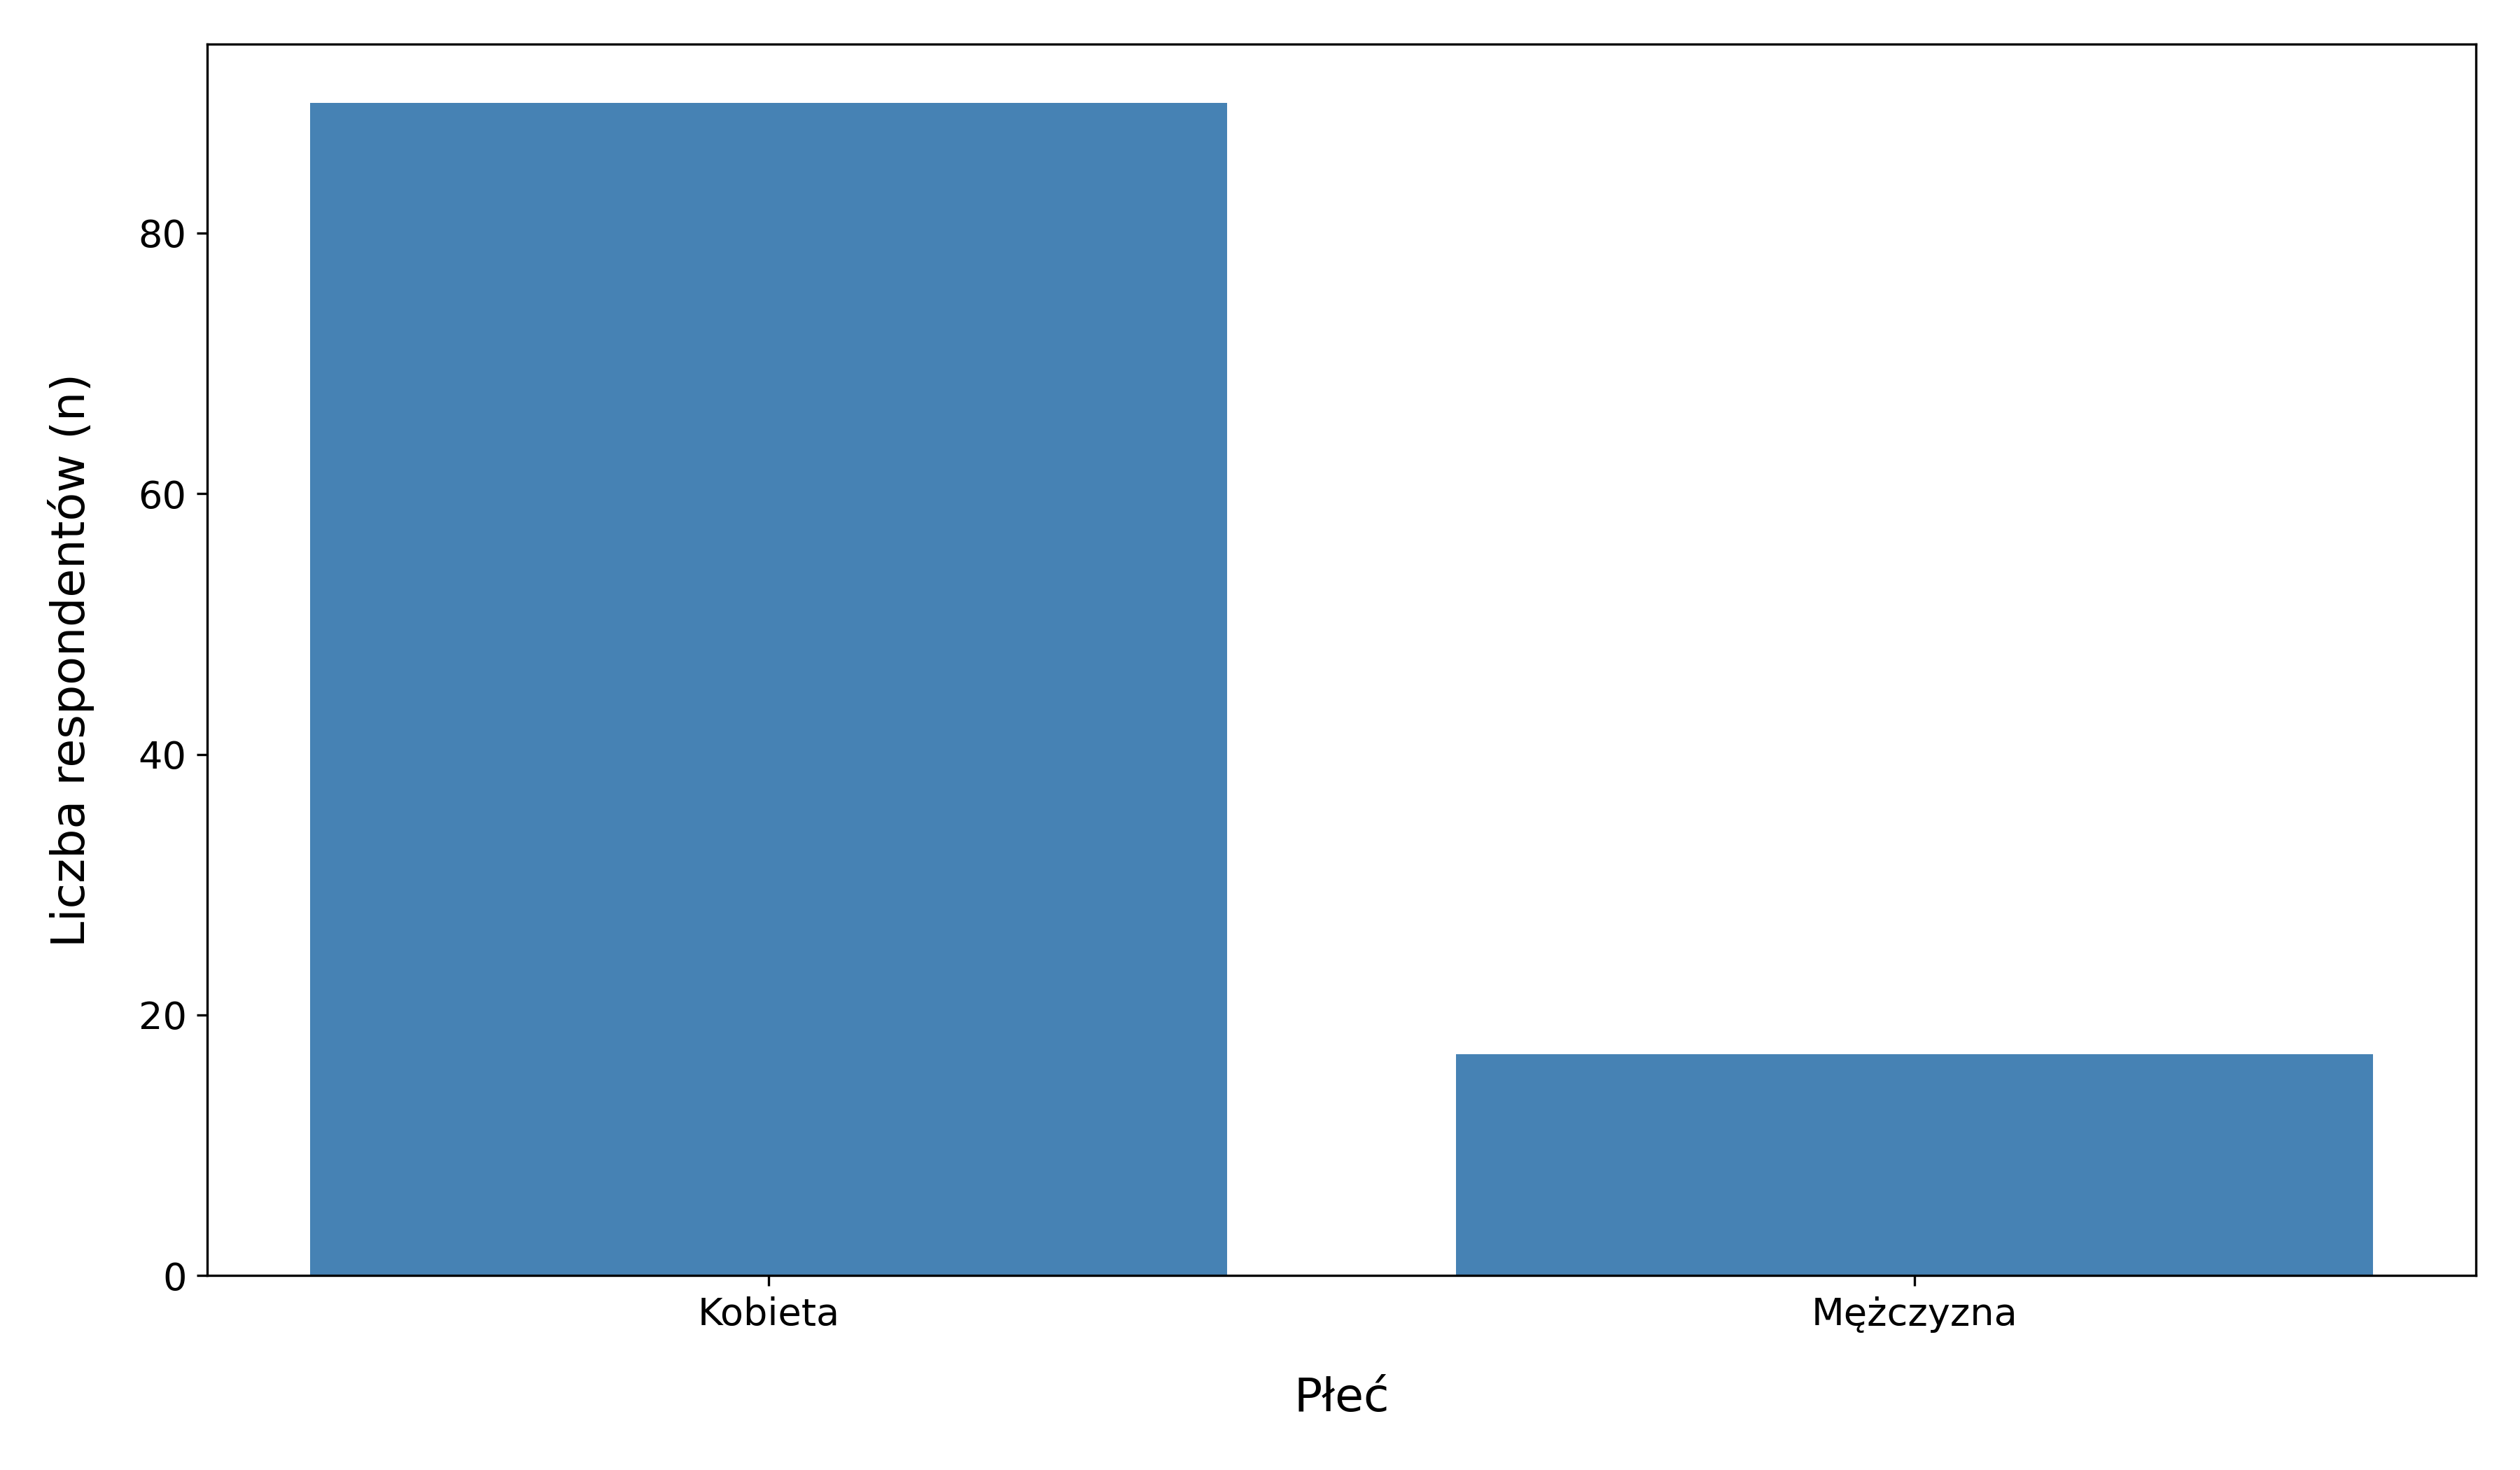
\includegraphics[width=\textwidth]{plots/plec-badanych.png}
    \centering
    \caption{Wykres słupkowy pokazujący liczbę respondentów poszczególnych płci.}
    \label{fig:plec}
\end{figure}

\begin{figure}
    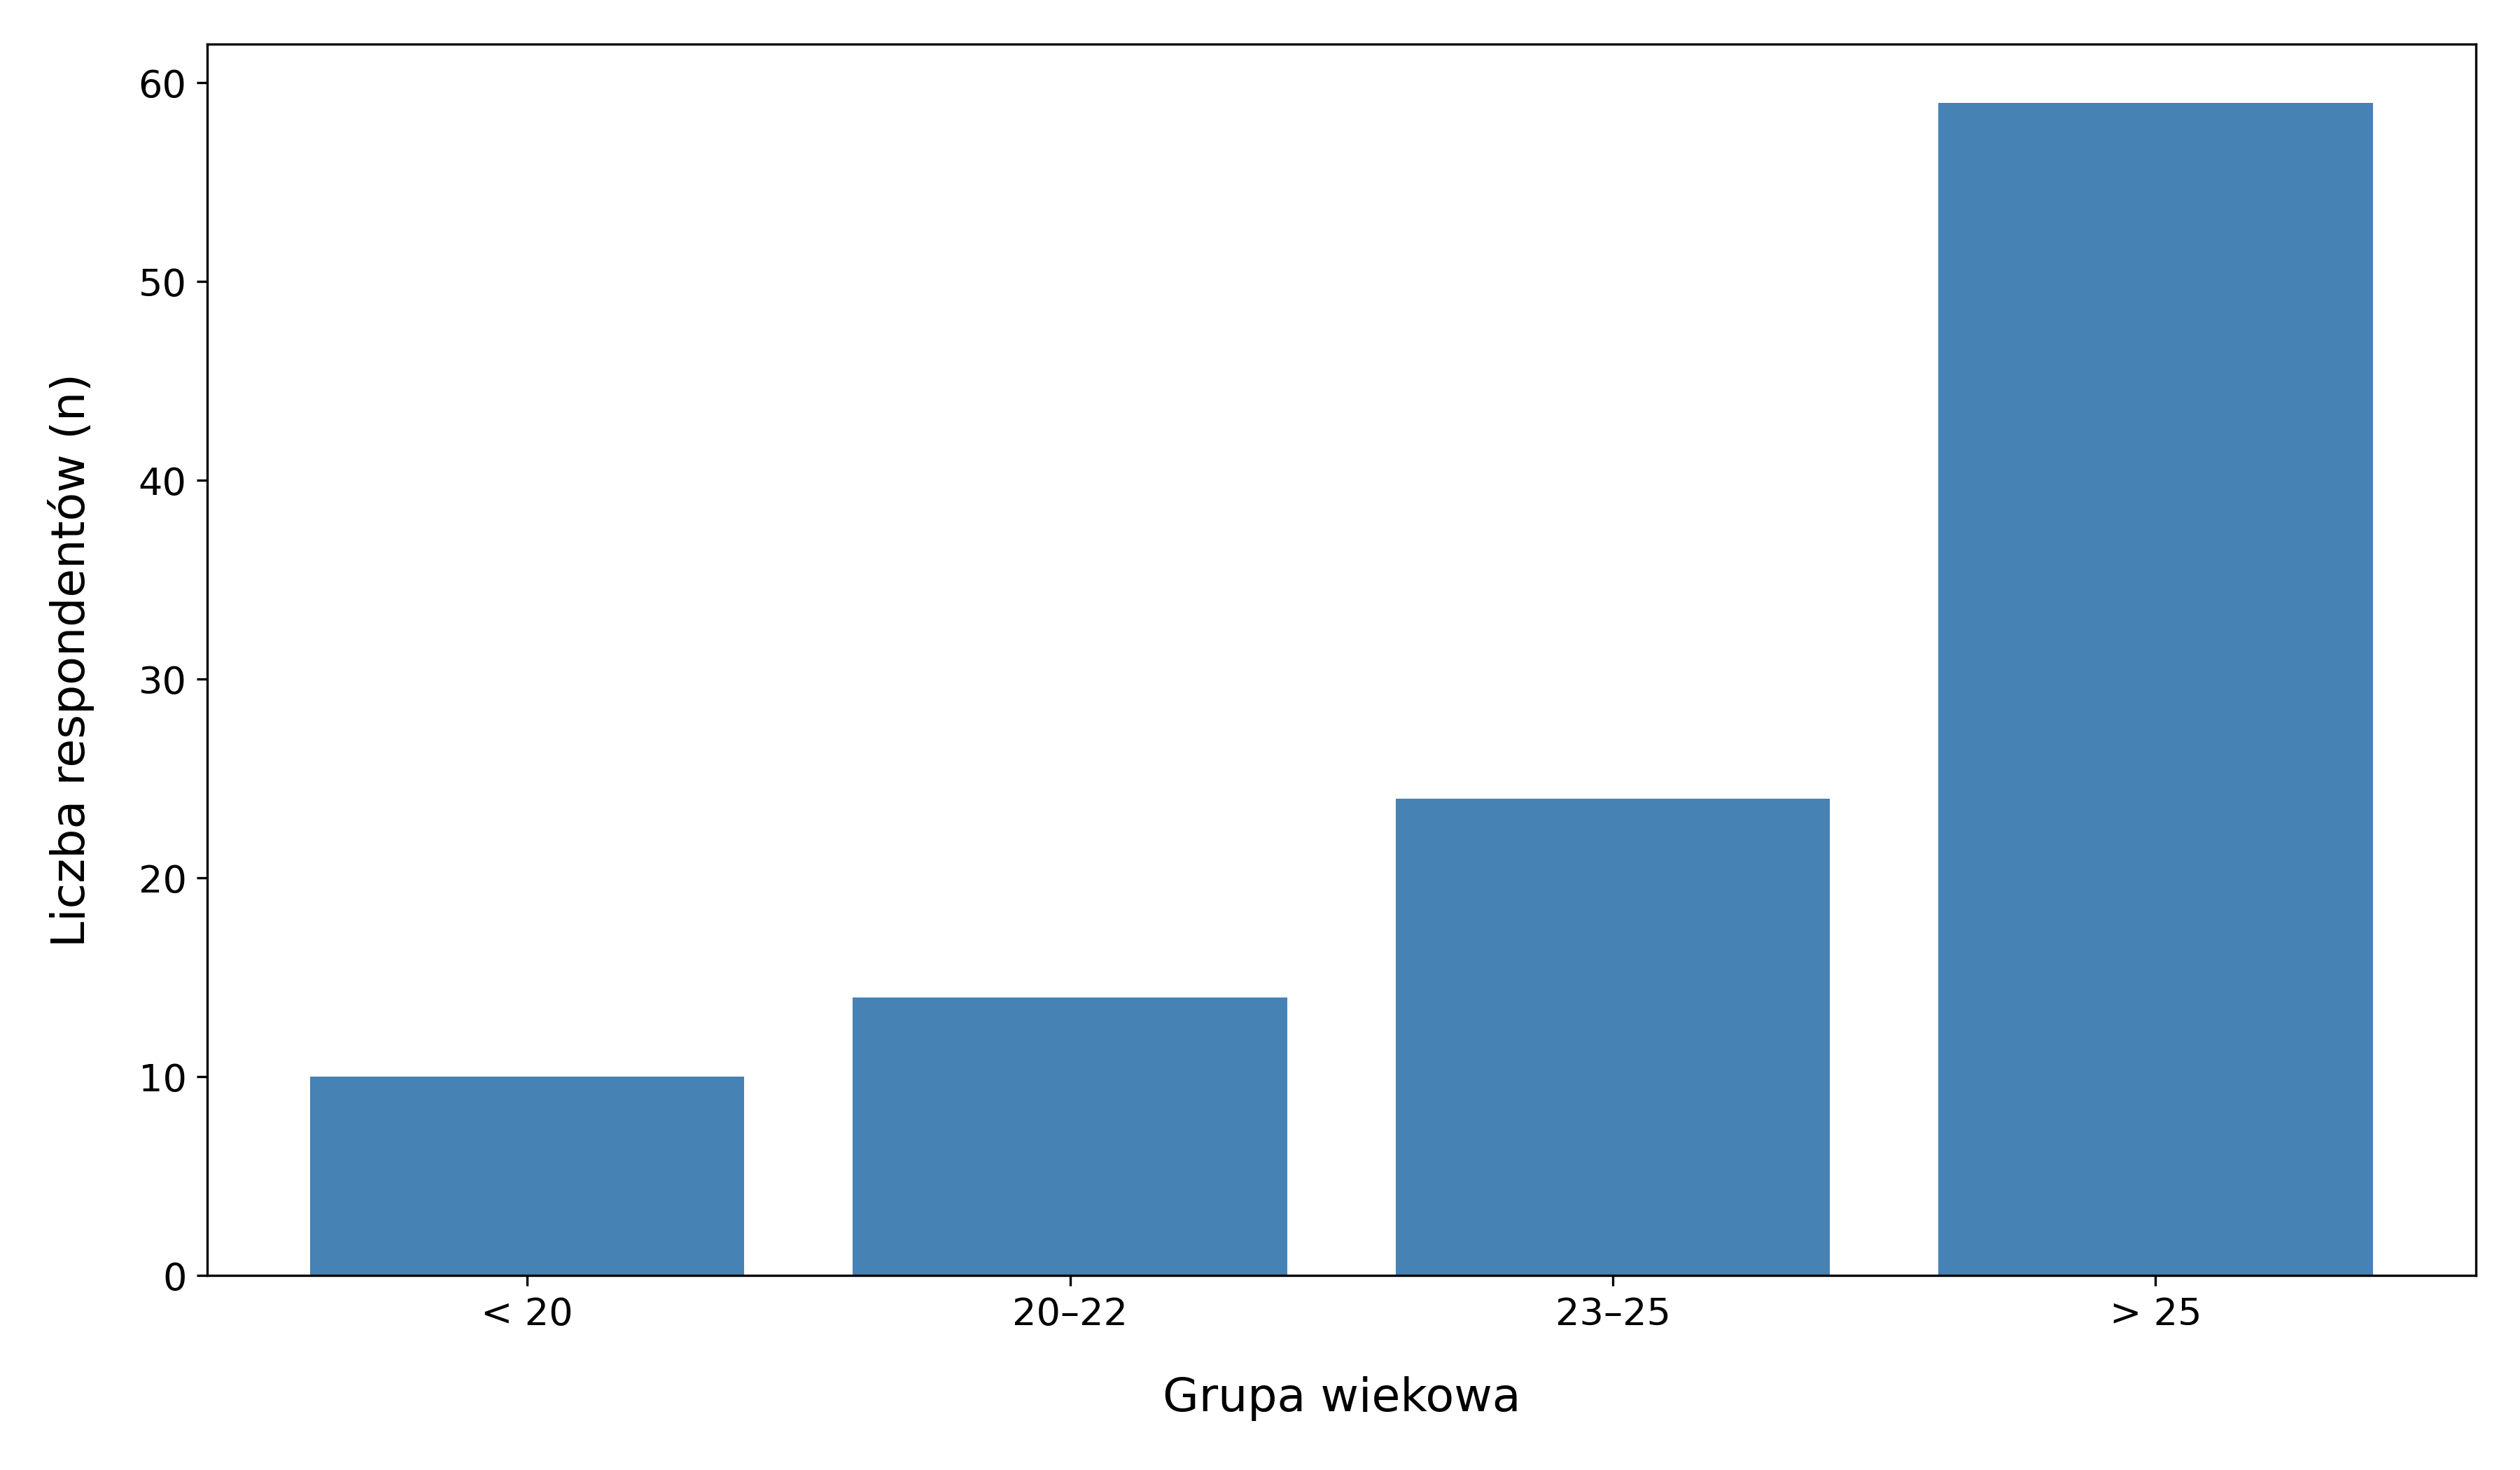
\includegraphics[width=\textwidth]{plots/wiek-badanych.png}
    \centering
    \caption{Wykres słupkowy pokazujący liczbę respondentów w poszczególnych grupach wiekowych.}
    \label{fig:wiek}
\end{figure}

\begin{figure}
    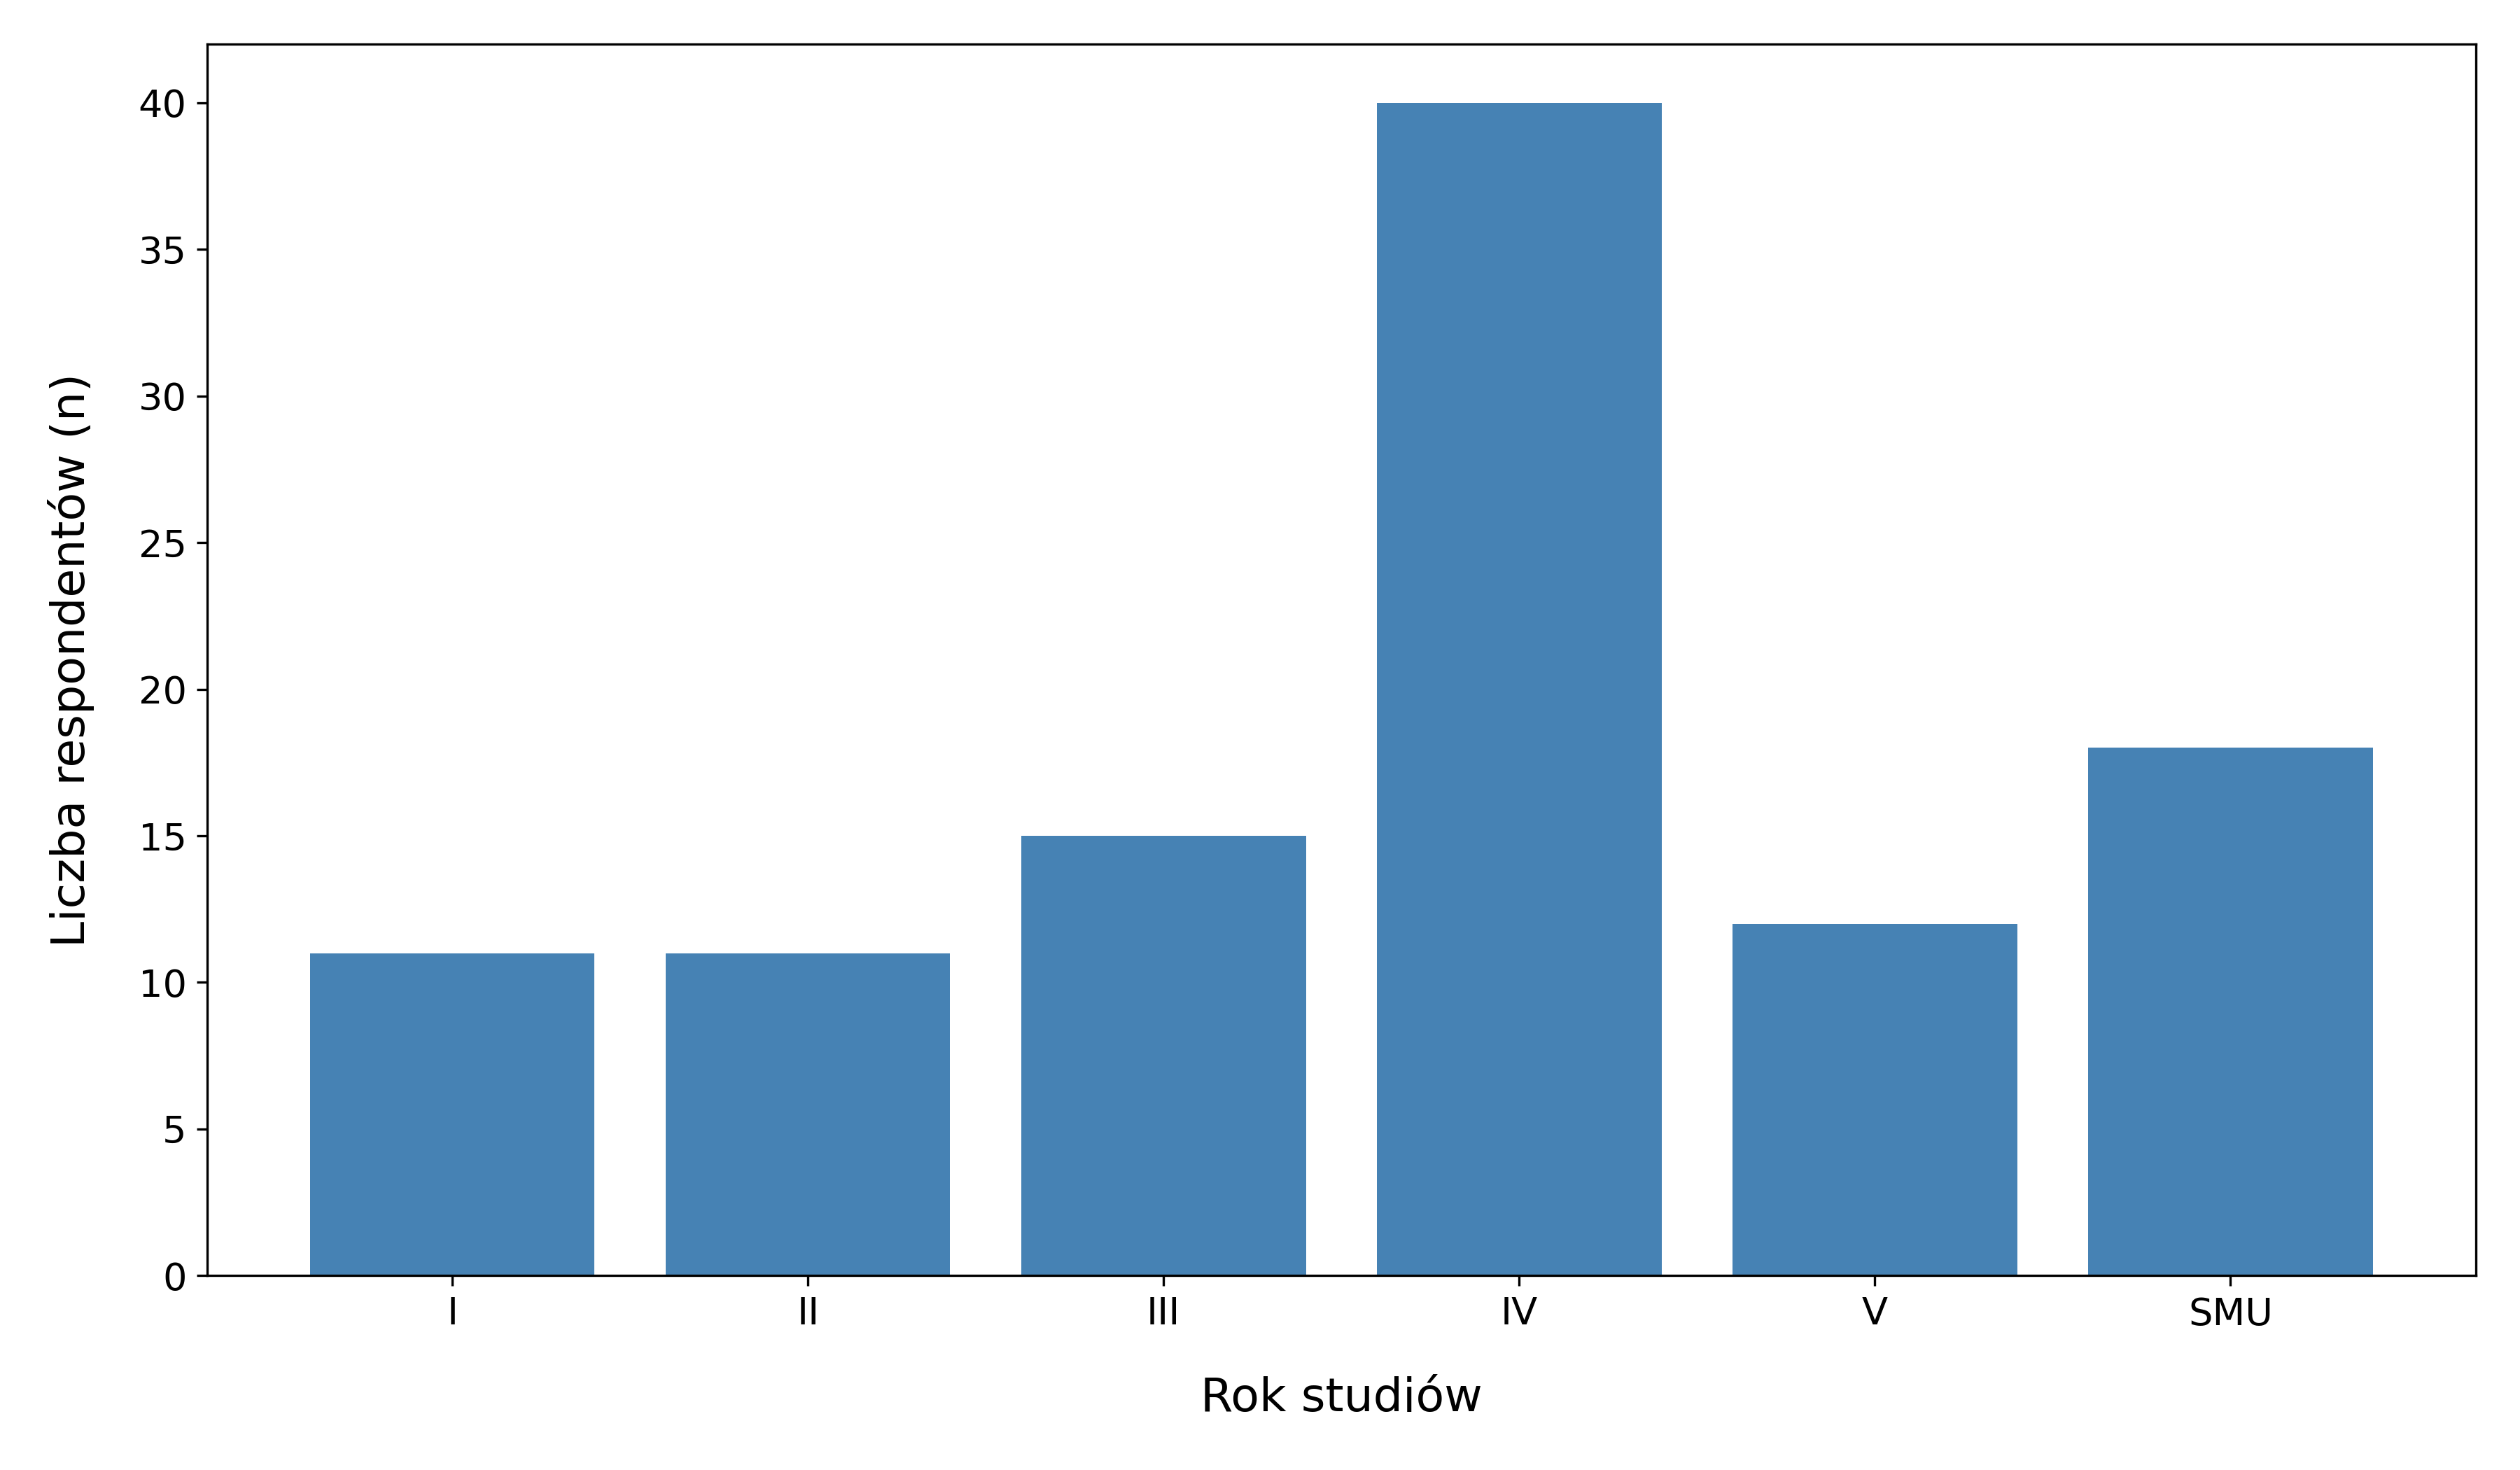
\includegraphics[width=\textwidth]{plots/rok-studiow.png}
    \centering
    \caption{Wykres słupkowy pokazujący liczbę respondentów na poszczególnych latach studiów. Zastosowane skróty: SMU - Studia magisterskie uzupełniające.}
    \label{fig:rok-studiow}
\end{figure}

\begin{figure}
    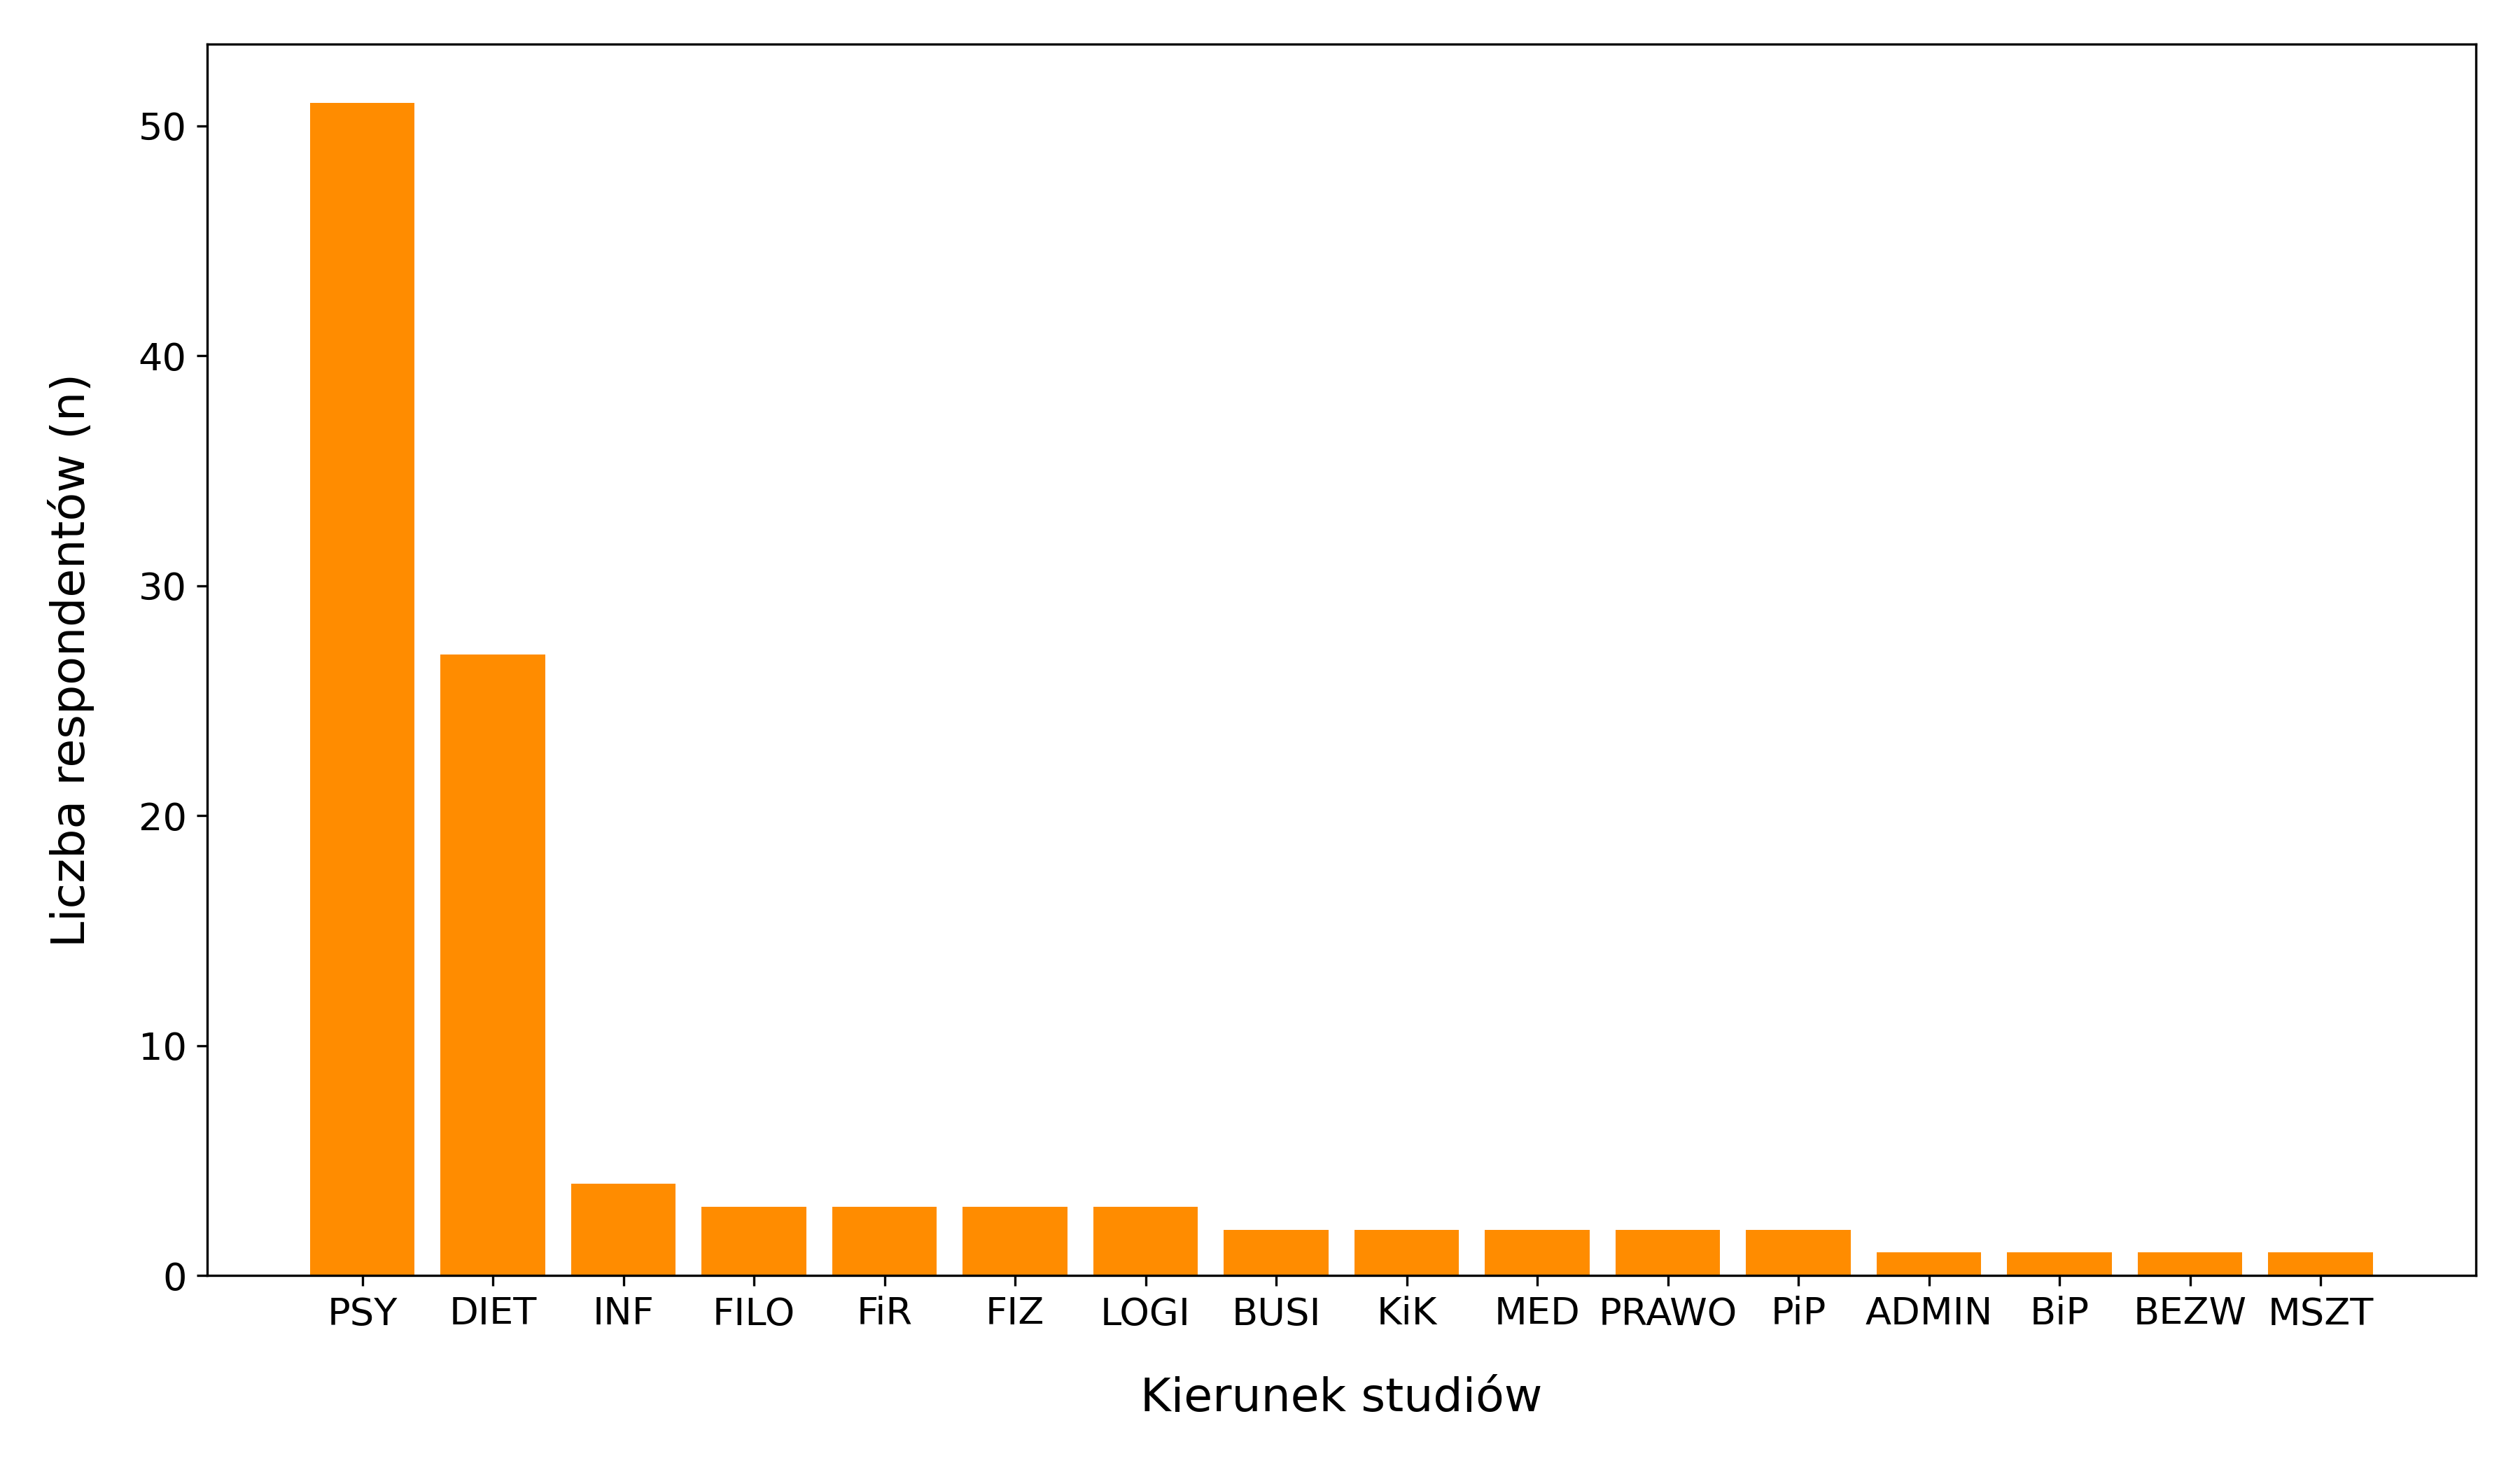
\includegraphics[width=\textwidth]{plots/kierunki-studiow.png}
    \centering
    \caption{Wykres słupkowy pokazujący liczbę respondentów ze względu na ich kierunek studiów. Zastosowane skróty: PSY - Psychologia, DIET - Dietetyka, INF - Informatyka, FILO - Filologia, FiR - Finanse i rachunkowość, FIZ - Fizjoterapia, LOGI - Logistyka, BUSI - Business, KiK - Kryminologia i kryminalistyka, MED - Medycyna, PRAWO - Prawo, PiP - Psychologia i psychoterapia, ADMIN - Administracja, BiP - Behawiorystyka i psychologia zwierząt, BEZW - Bezpieczeństwo wewnętrzne, MSZT - Mediacja sztuki).}
    \label{fig:kierunki-studiow}
\end{figure}

\begin{figure}
    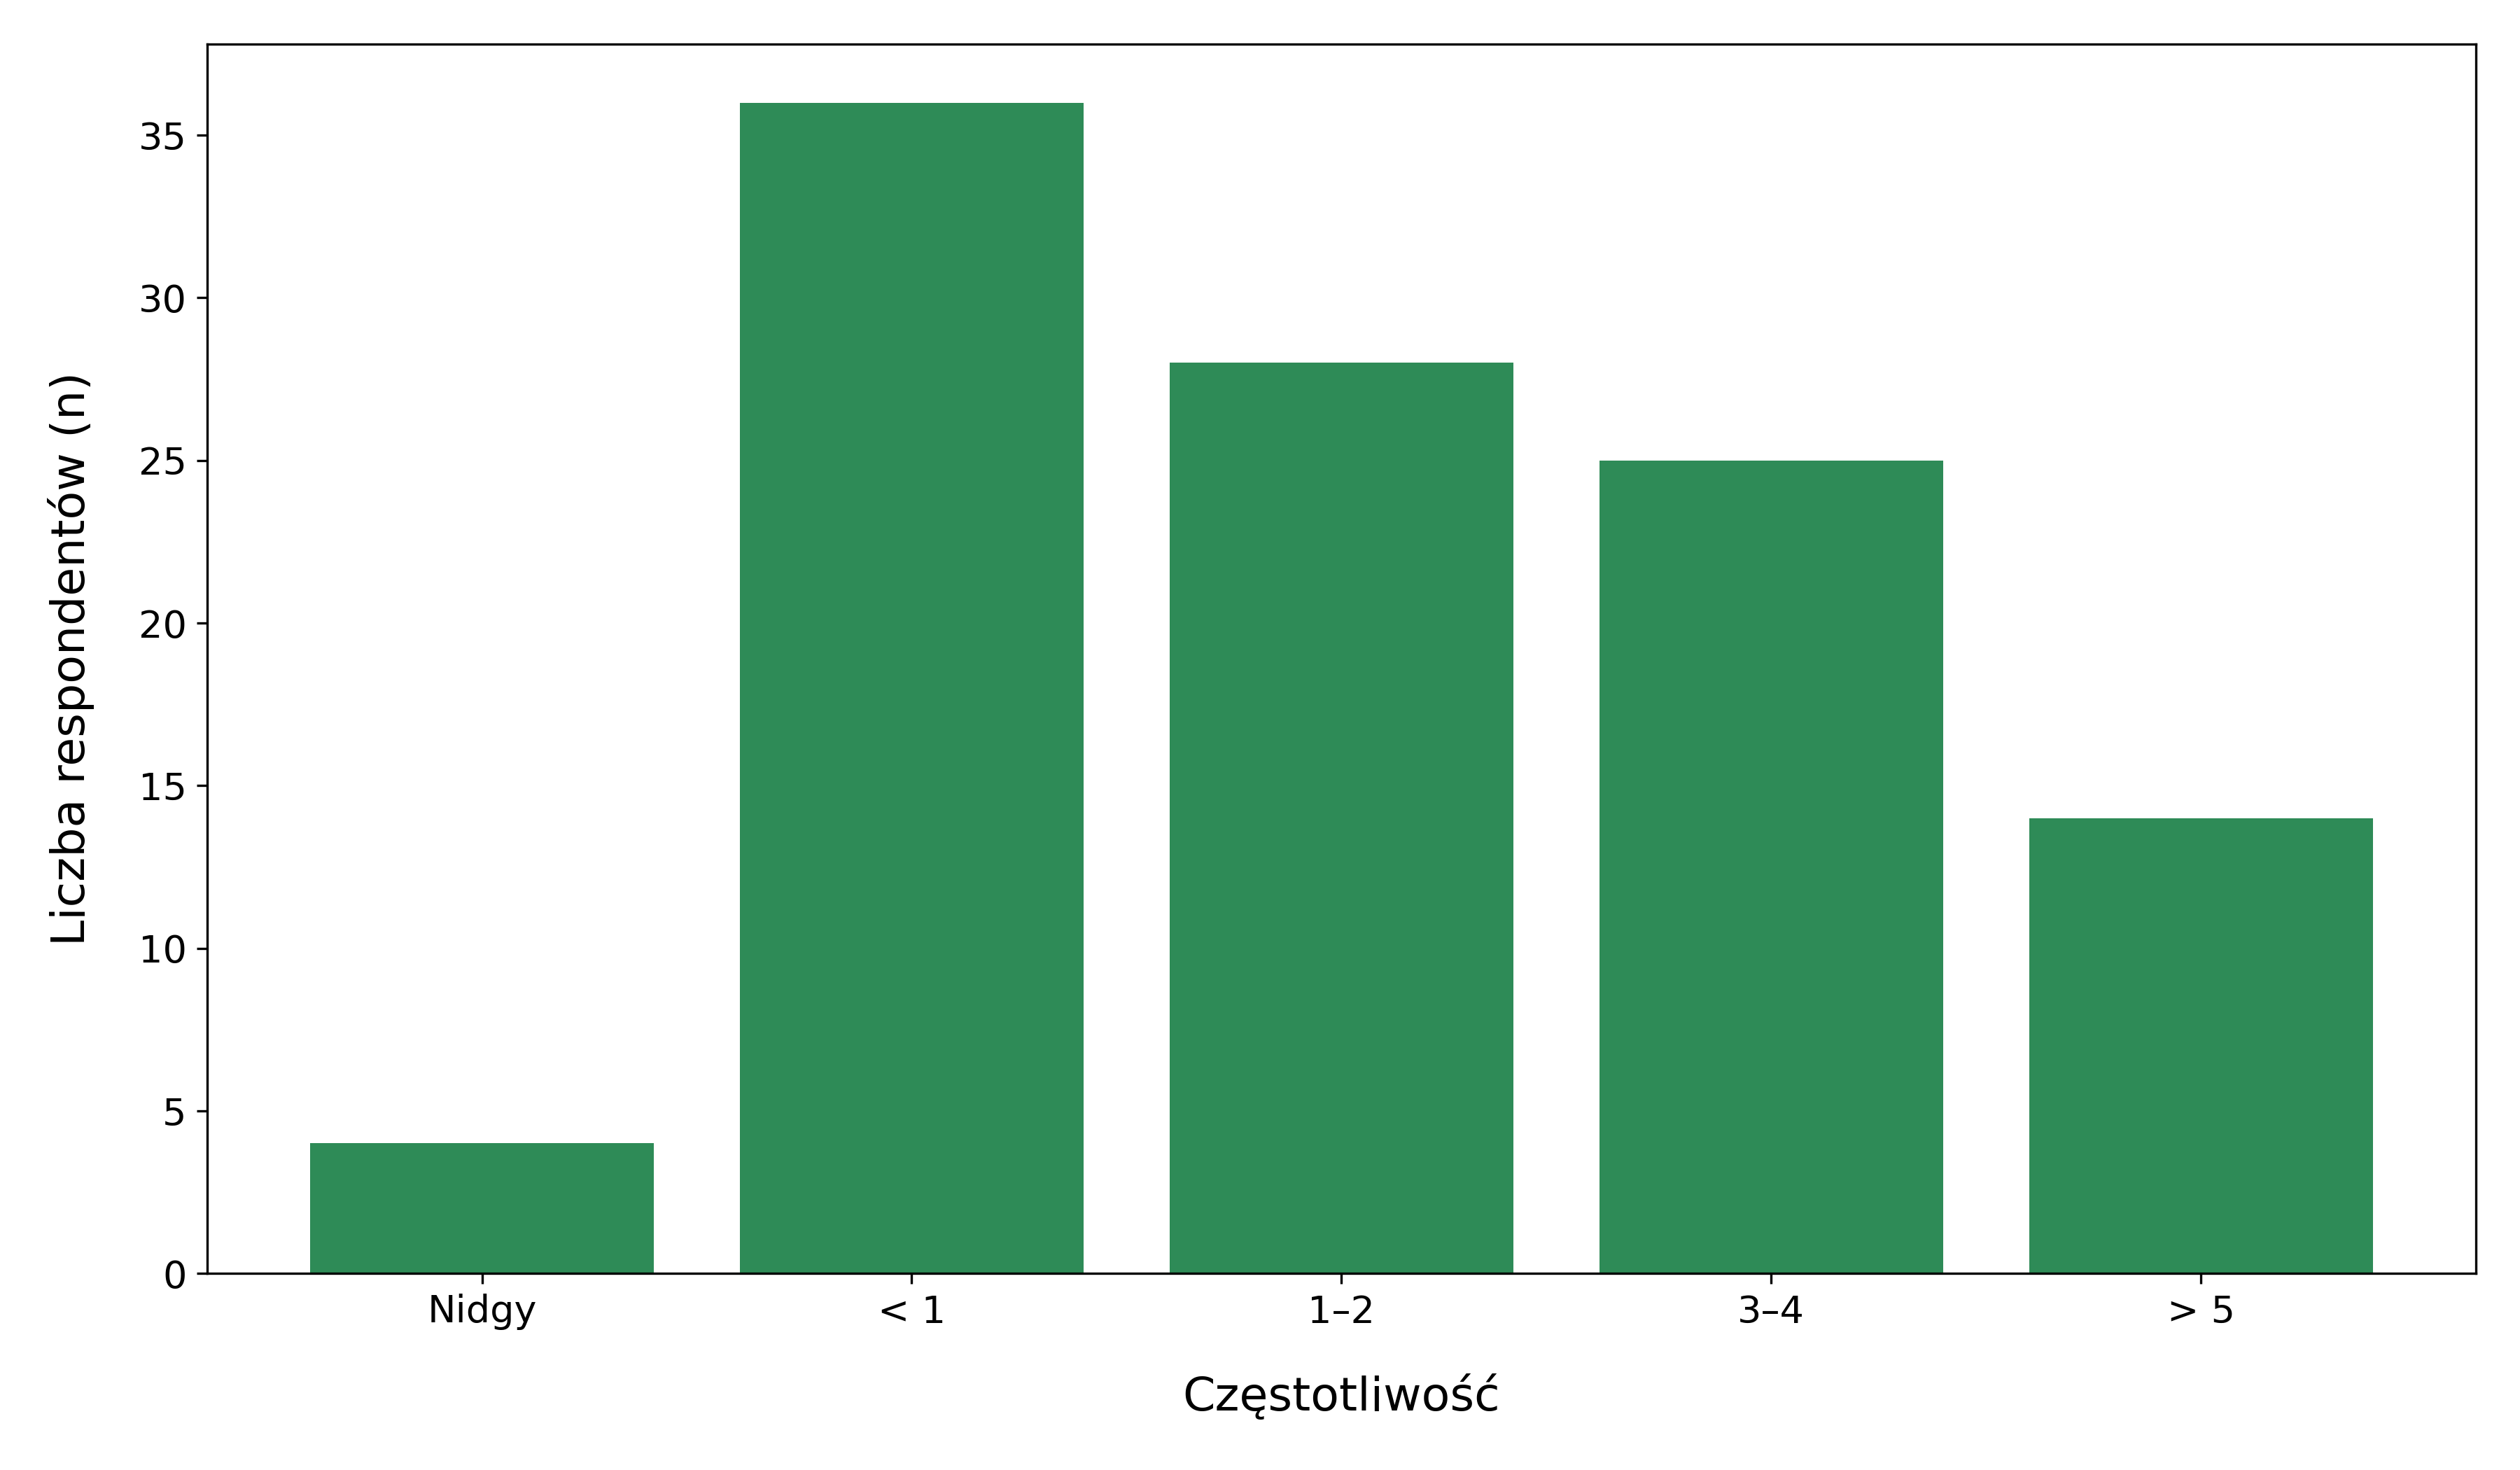
\includegraphics[width=\textwidth]{plots/aktywnosc-fizyczna.png}
    \centering
    \caption{Wykres słupkowy pokazujący częstość wykonywania aktywności fizycznej wśród respondentów.}
    \label{fig:aktywnosc-fizyczna}
\end{figure}


\subsection{Częstość stosowania suplementów}

% Należy przedstawić, ilu studentów aktualnie stosuje suplementy diety.

% Czy aktualnie stosujesz suplementy?, n, %

\begin{table}[h!]
    \centering
    \caption{Aktualne stosowanie suplementów}
    \label{tab:akt-stos-supl}
    \begin{tabular}{|l|l|l|}
        \hline
        Aktualne stosowanie suplementów & n & \% \\
        \hline
        \hline
        Tak & 97 & 90.7 \\
        \hline
        Nie & 10 & 9.3 \\
        \hline
    \end{tabular}
\end{table}

\begin{figure}
    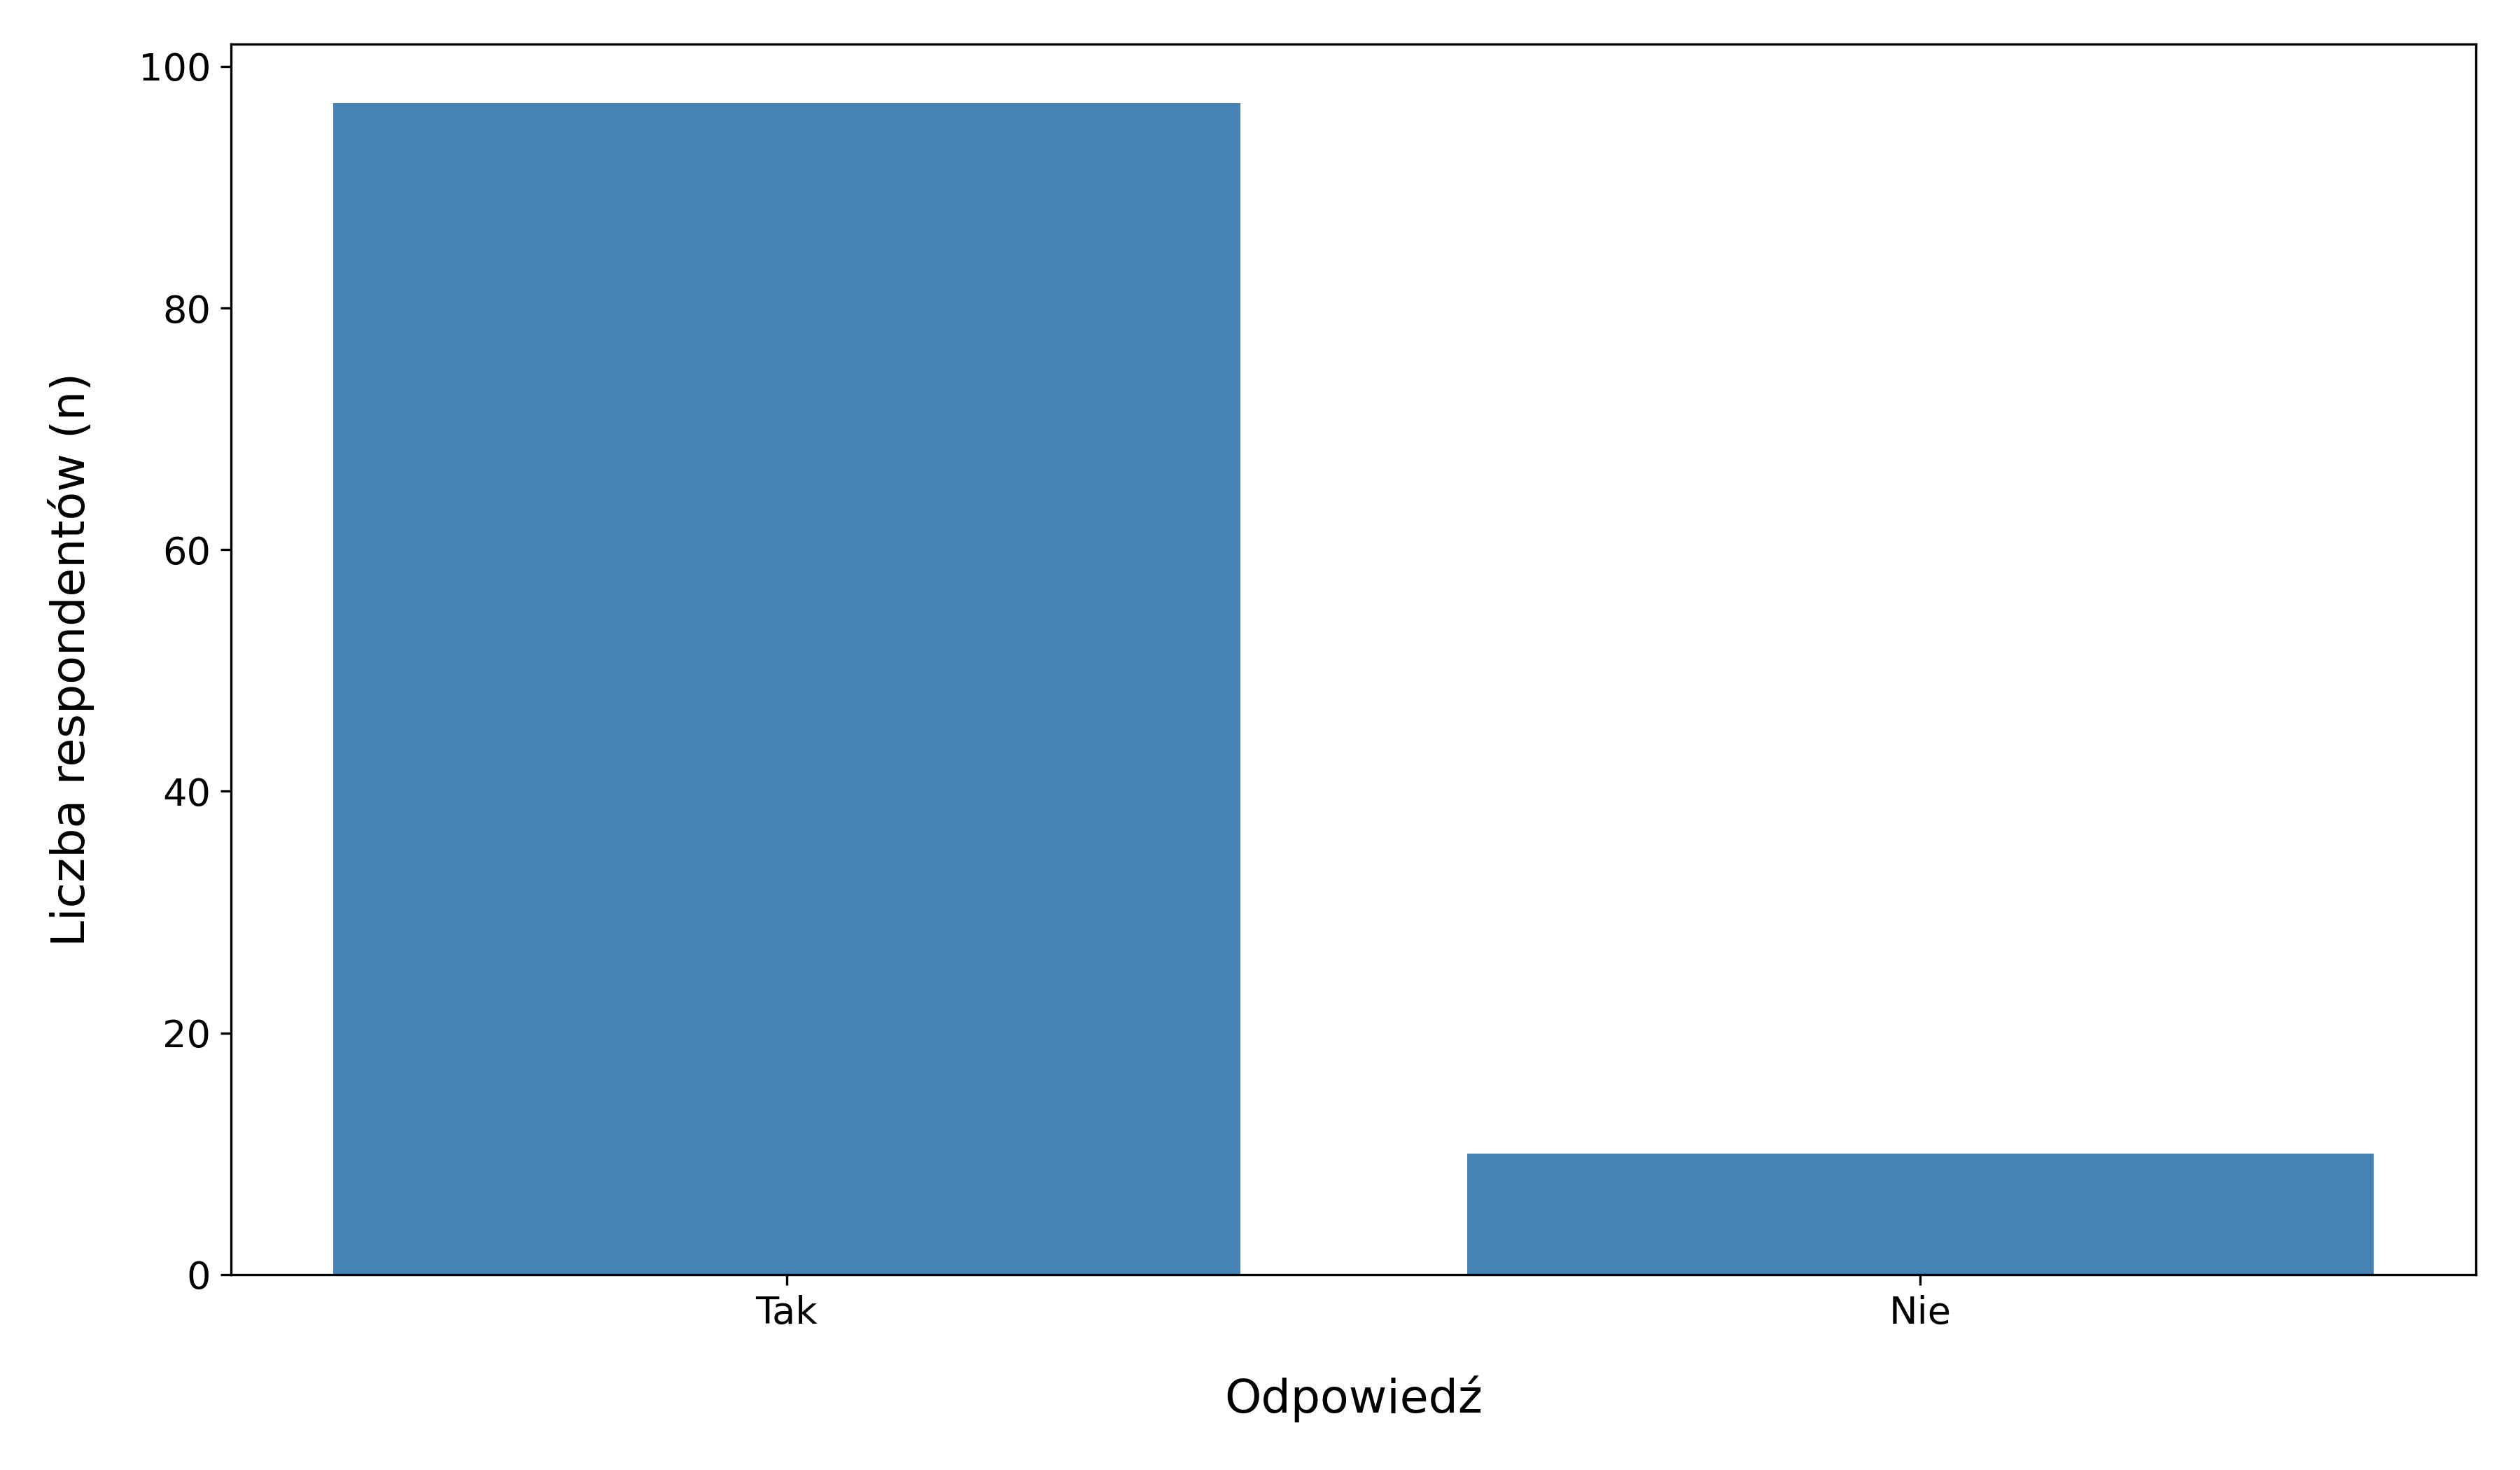
\includegraphics[width=\textwidth]{plots/aktualne-suplementy.png}
    \centering
    \caption{Wykres słupkowy pokazujący aktualne stosowanie suplementów w grupie badawczej.}
    \label{fig:akt-stos-supl}
\end{figure}

% NOTE
% Adjust all below based on whether participant take suplements

% Częstość stosowania suplementów

\begin{table}[h!]
    \centering
    \caption{Częstość stosowanie suplementów}
    \label{tab:cze-stos-supl}
    \begin{tabular}{|l|l|l|}
        \hline
        Częstość stosowania & n & \% \\
        \hline
        \hline
        Codziennie & 63 & 64.95 \\
        \hline
        Kilka razy w tygodniu & 21 & 21.65 \\
        \hline
        Kilka razy w miesiącu & 3 & 3.1 \\
        \hline
        Sporadycznie & 10 & 10.3 \\
        \hline
    \end{tabular}
\end{table}

\begin{figure}
    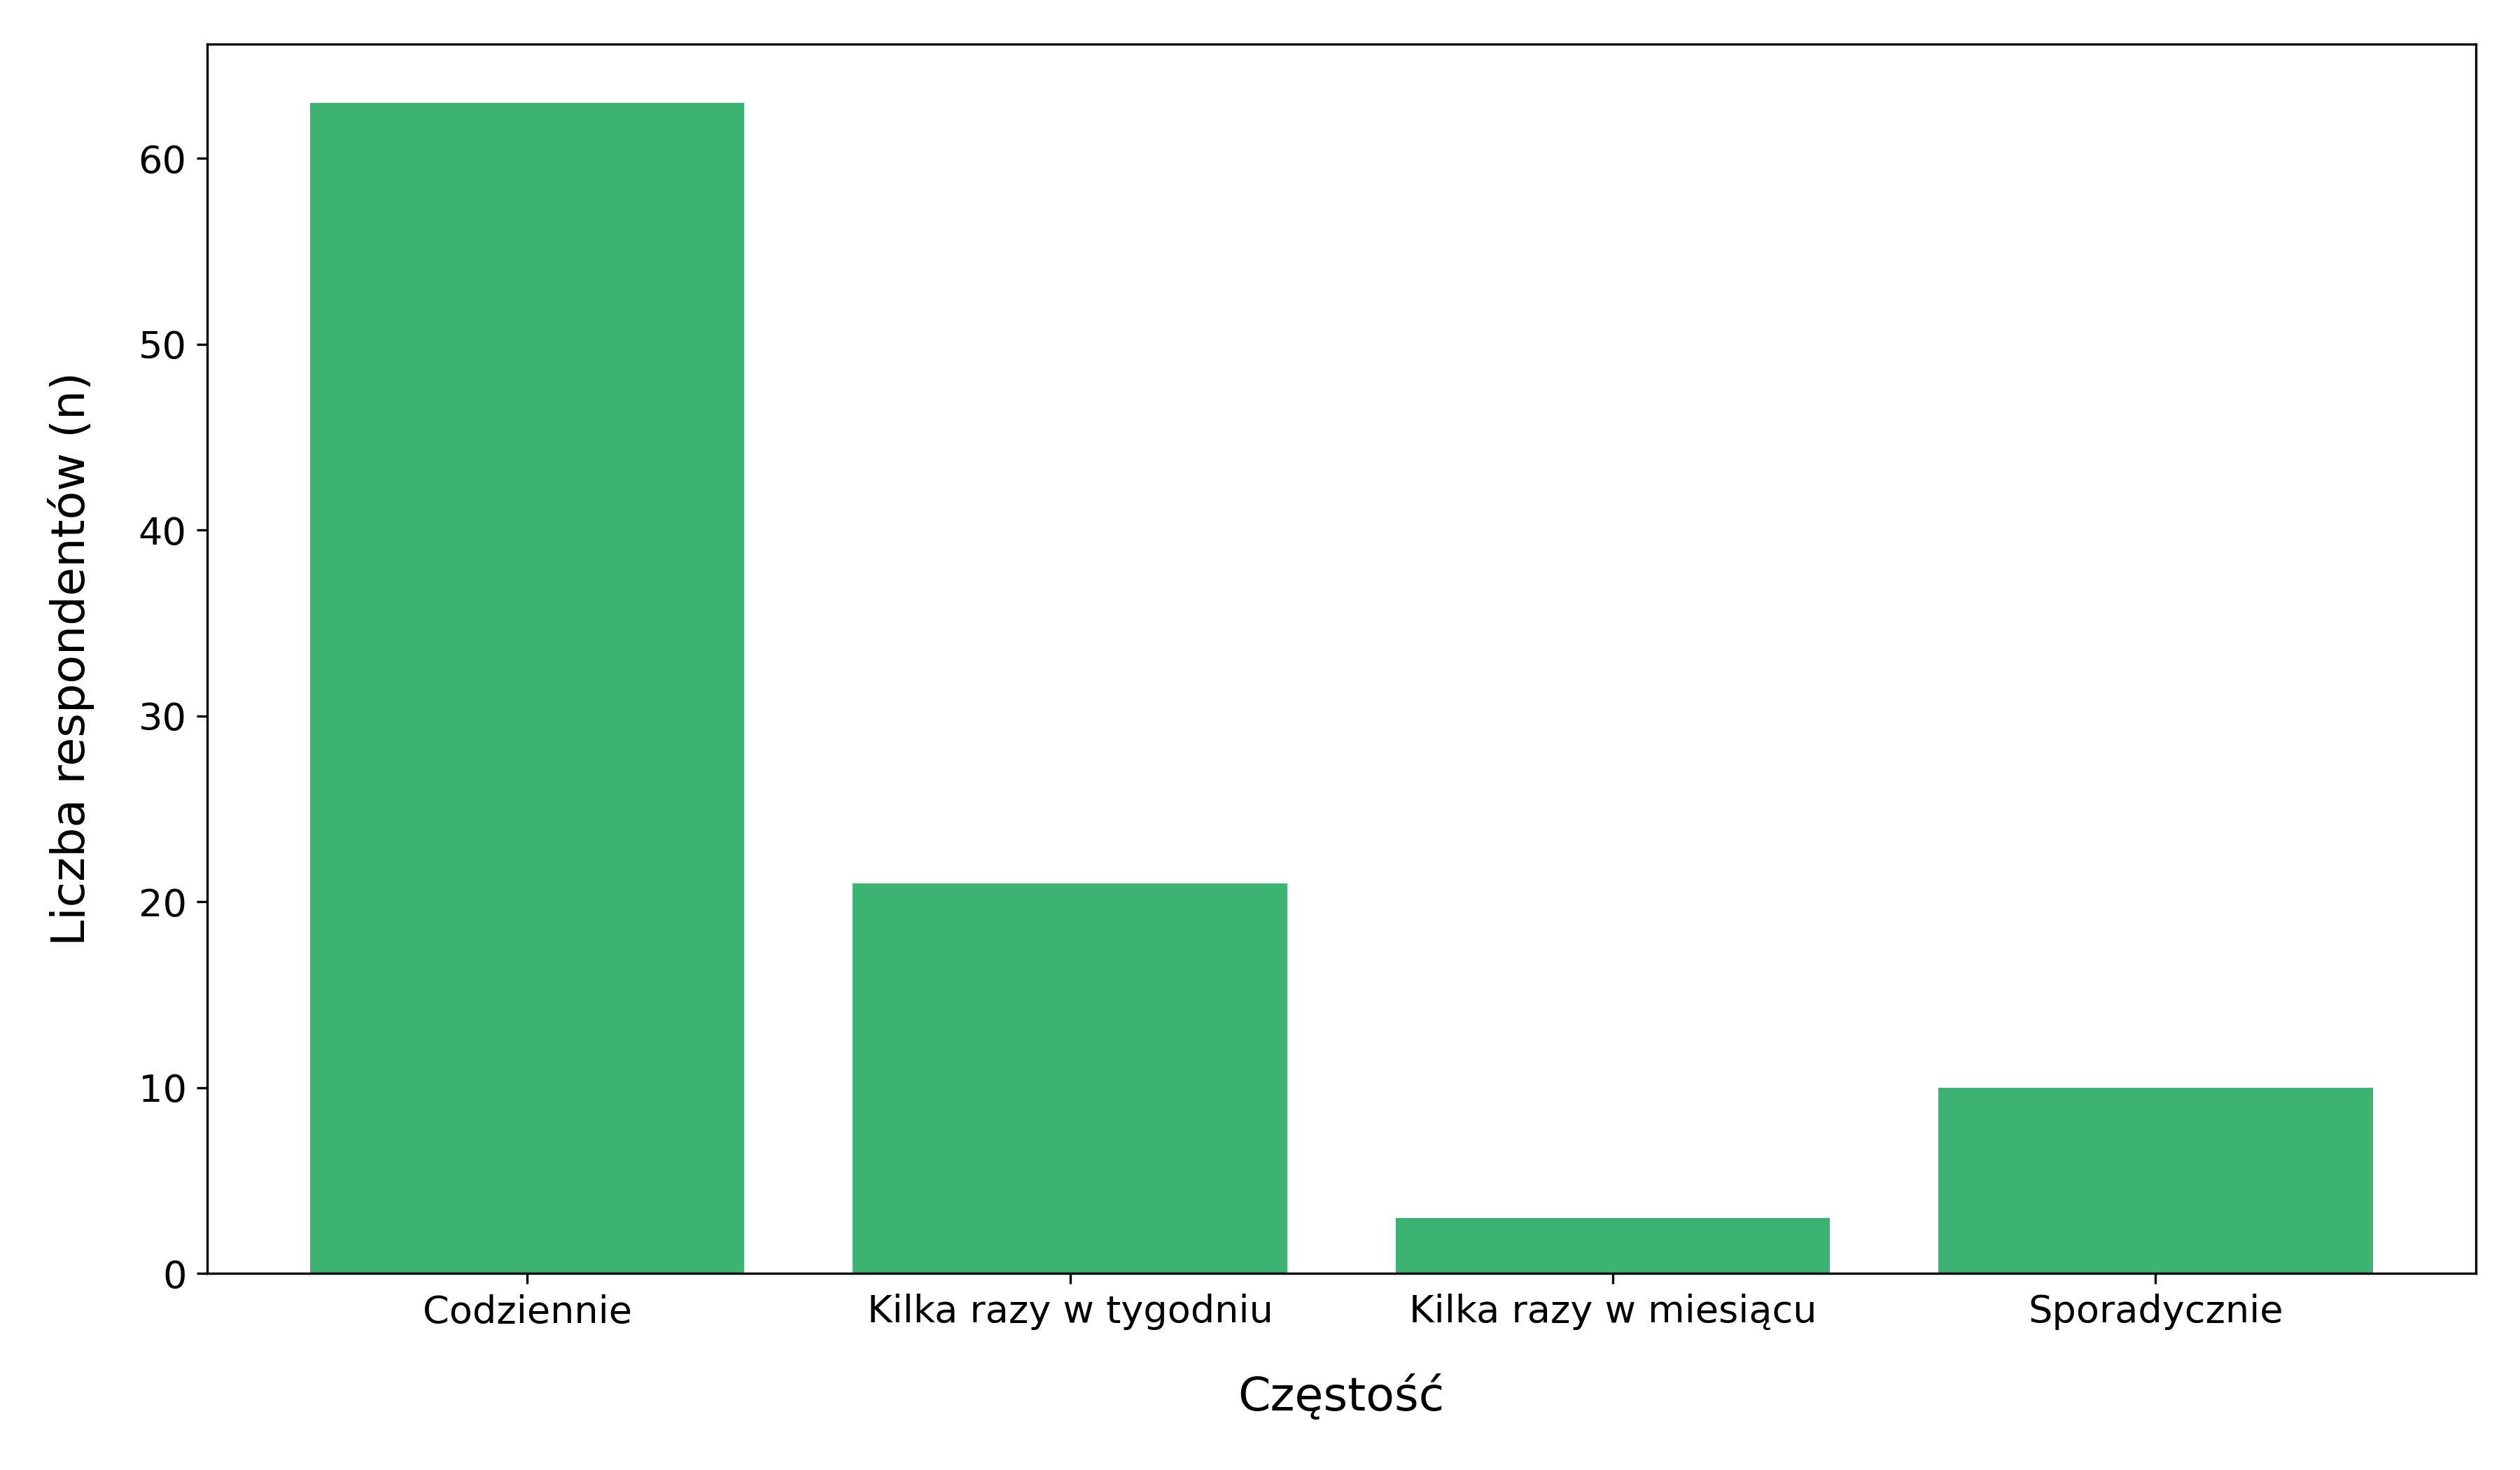
\includegraphics[width=\textwidth]{plots/czestosc-suplementow.png}
    \centering
    \caption{Wykres słupkowy pokazujący częstość stosowania suplementów w grupie badawczej.}
    \label{fig:cze-stos-supl}
\end{figure}

% Czas stosowania suplementów

\begin{table}[h!]
    \centering
    \caption{Czas stosowanie suplementów}
    \label{tab:czas-stos-supl}
    \begin{tabular}{|l|l|l|}
        \hline
        Czas stosowania & n & \% \\
        \hline
        \hline
        < 3 miesięcy & 15 & 15.46 \\
        \hline
        3–12 miesięcy & 23 & 23.71 \\
        \hline
        1–3 lata & 22 & 22.68 \\
        \hline
        >3 lat & 37 & 38.15 \\
        \hline
    \end{tabular}
\end{table}

\begin{figure}
    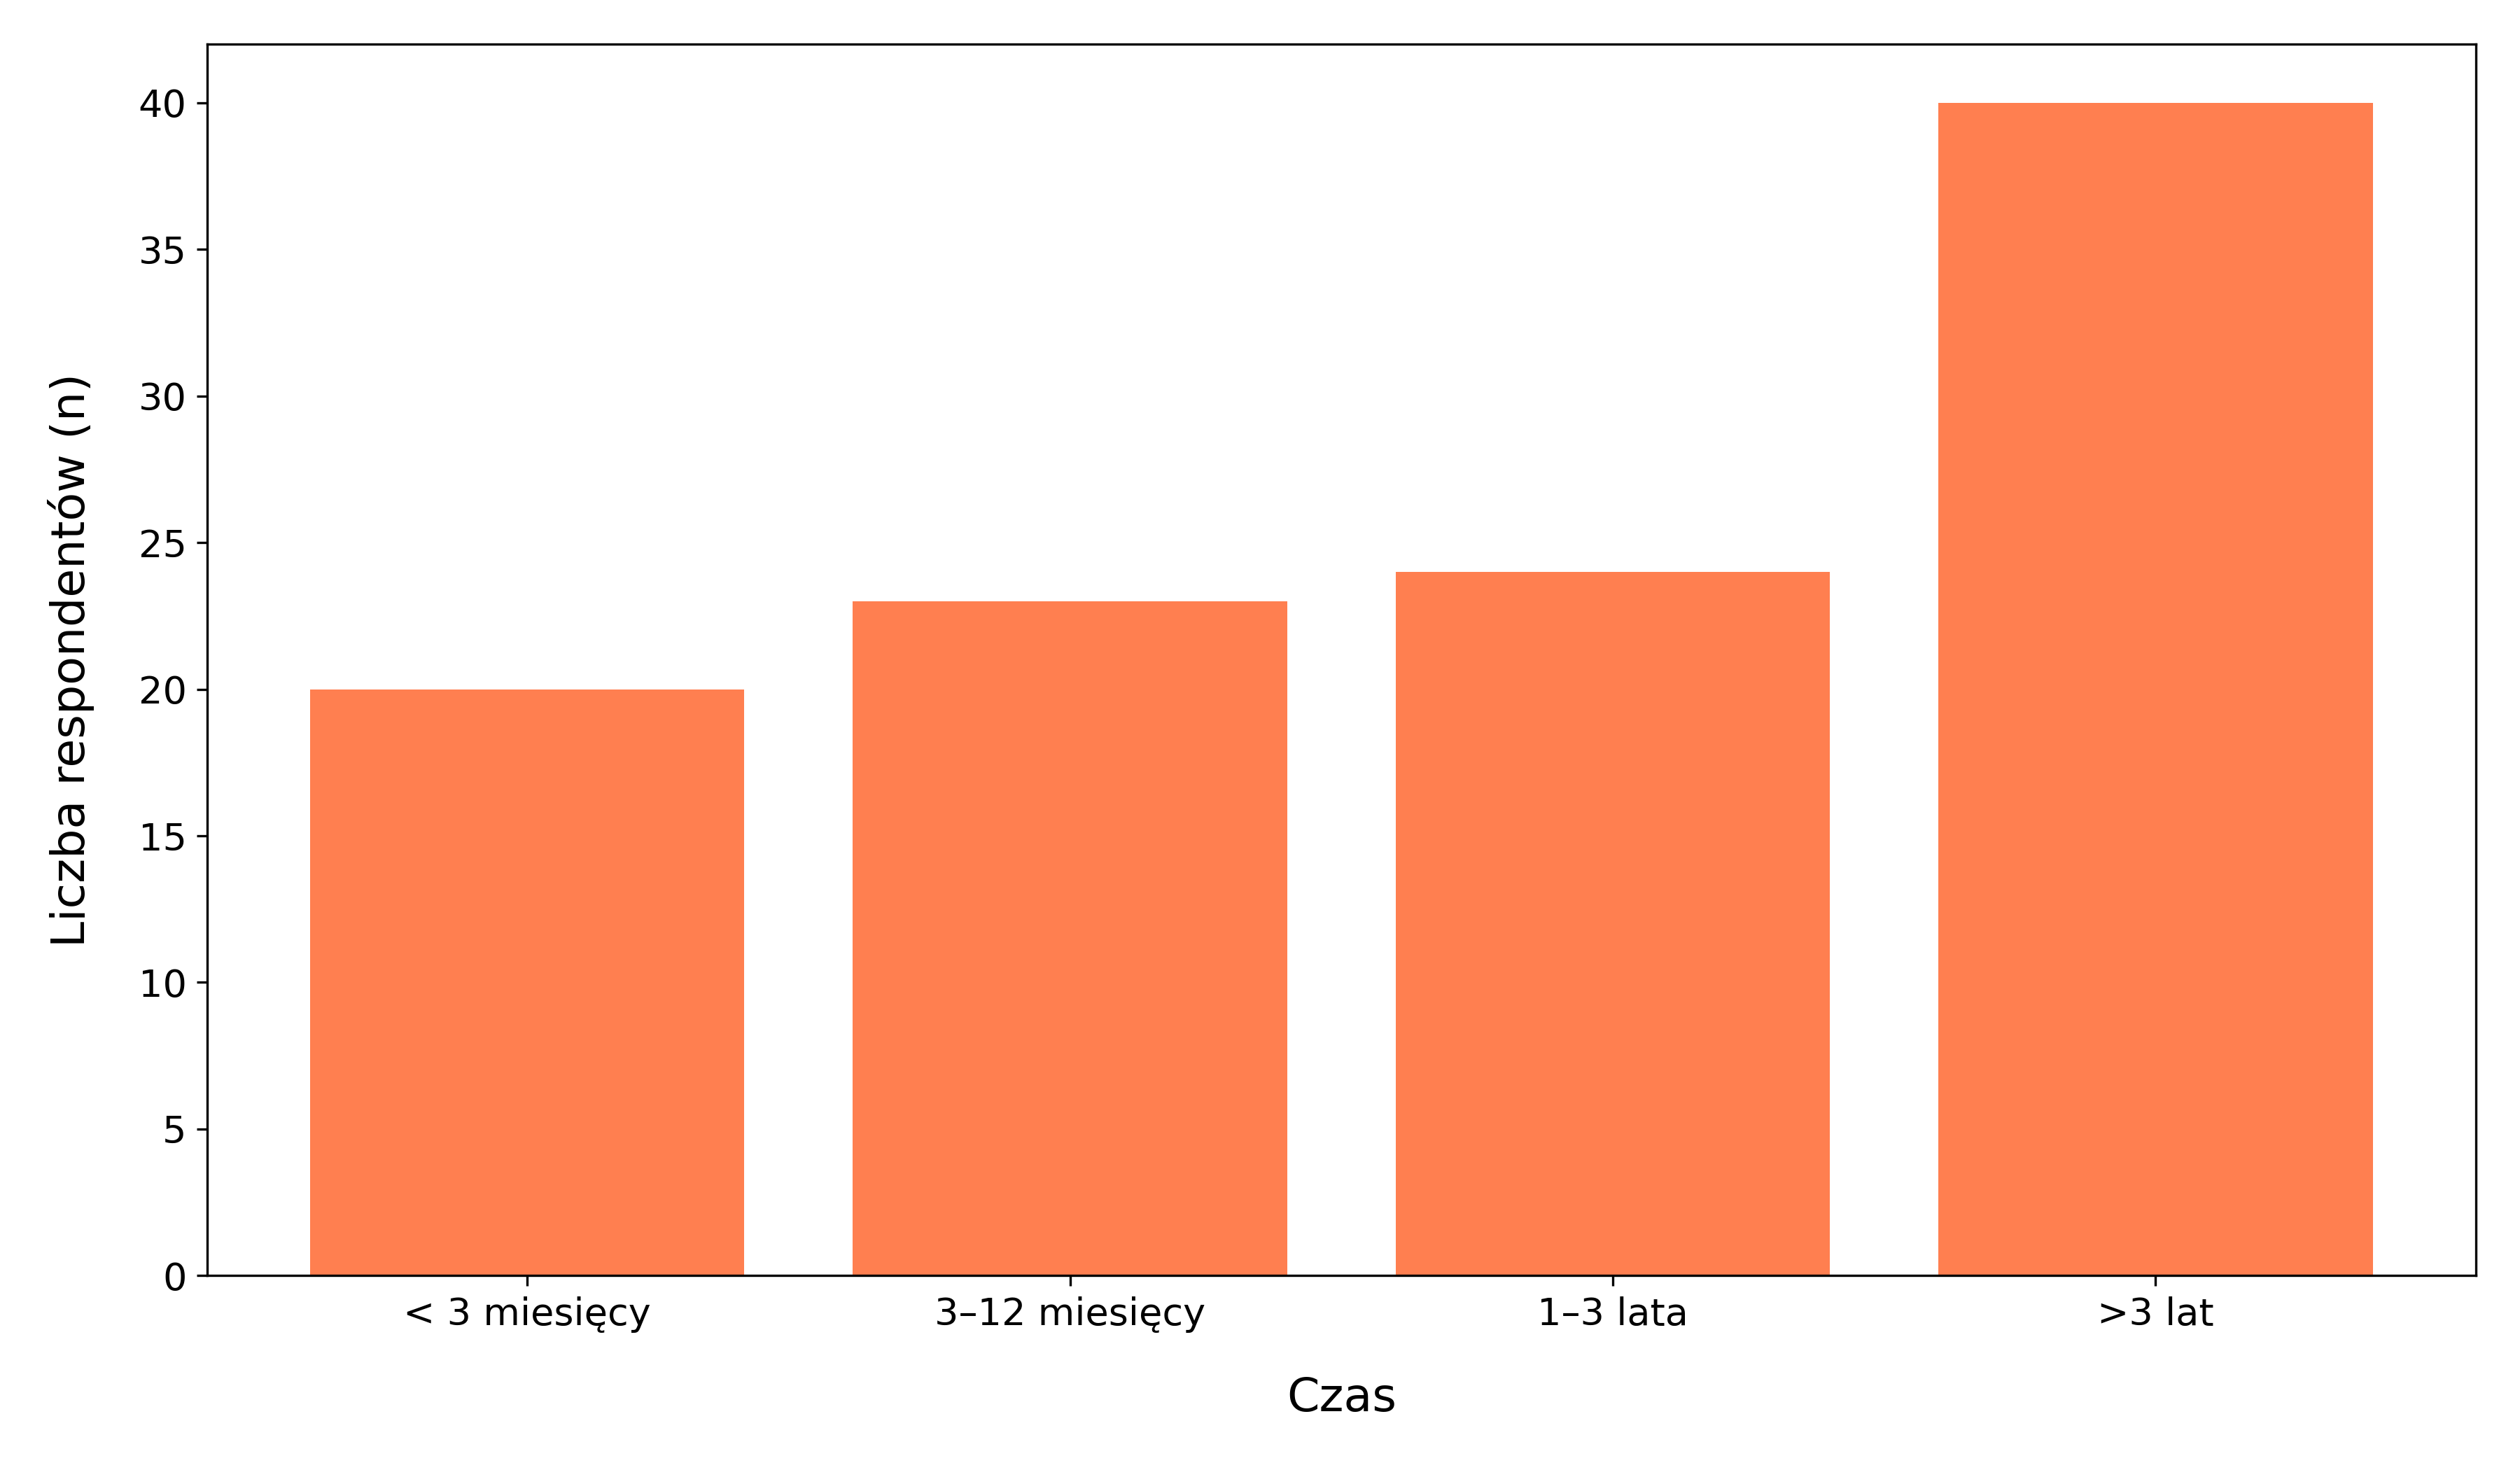
\includegraphics[width=\textwidth]{plots/czas-suplementow.png}
    \centering
    \caption{Wykres słupkowy pokazujący czas stosowania suplementów w grupie badawczej.}
    \label{fig:czas-stos-supl}
\end{figure}

% Wykres słupkowy pokazujący odsetek osób stosujących i niestosujących suplementów.
% Dodatkowo
% Wśród osób stosujących suplementy należy opisać:
%     + jak często je stosują,
%     + od jak dawna je stosują.

% Statystyka
% Statystyka opisowa:
%     + n,
%     + %.
% Można później wykorzystać zmienną „stosowanie suplementów: tak/nie” do analiz zależności.

\subsection{Rodzaje stosowanych suplementów}

% To pytanie wielokrotnego wyboru, więc procenty należy liczyć względem liczby osób stosujących suplementy, a nie względem wszystkich odpowiedzi.
% Należy pokazać, które suplementy były wybierane najczęściej.

% Wykres
% Najlepszy będzie poziomy wykres słupkowy - ranking suplementów od najczęściej do najrzadziej wybieranych.

% Najczęściej stosowane suplementy

\begin{table}[h!]
    \centering
    \caption{Rodzaje stosowanych suplementów}
    \label{tab:rodz-stos-supl}
    \begin{tabular}{|l|l|l|}
        \hline
        Rodzaj suplementu & n  & \% respondentów \\
        \hline
        \hline
        Witamina D & 79 & 81.4 \\
        \hline
        Kwasy omega-3 & 59 & 60.8 \\
        \hline
        Magnez & 48 & 49.4 \\
        \hline
        Probiotyki & 40 & 41.2 \\
        \hline
        Inne odpowiedzi & 39 & 40.2 \\
        \hline
        Multiwitaminy & 32 & 32.9 \\
        \hline
        Witamina C & 31 & 31.9 \\
        \hline
        Białko & 24 & 24.7 \\
        \hline
        Kreatyna & 15 & 15.4 \\
        \hline
        Adaptogeny (np. ashwagandha) & 11 & 11.3 \\
        \hline
    \end{tabular}
\end{table}

\begin{figure}
    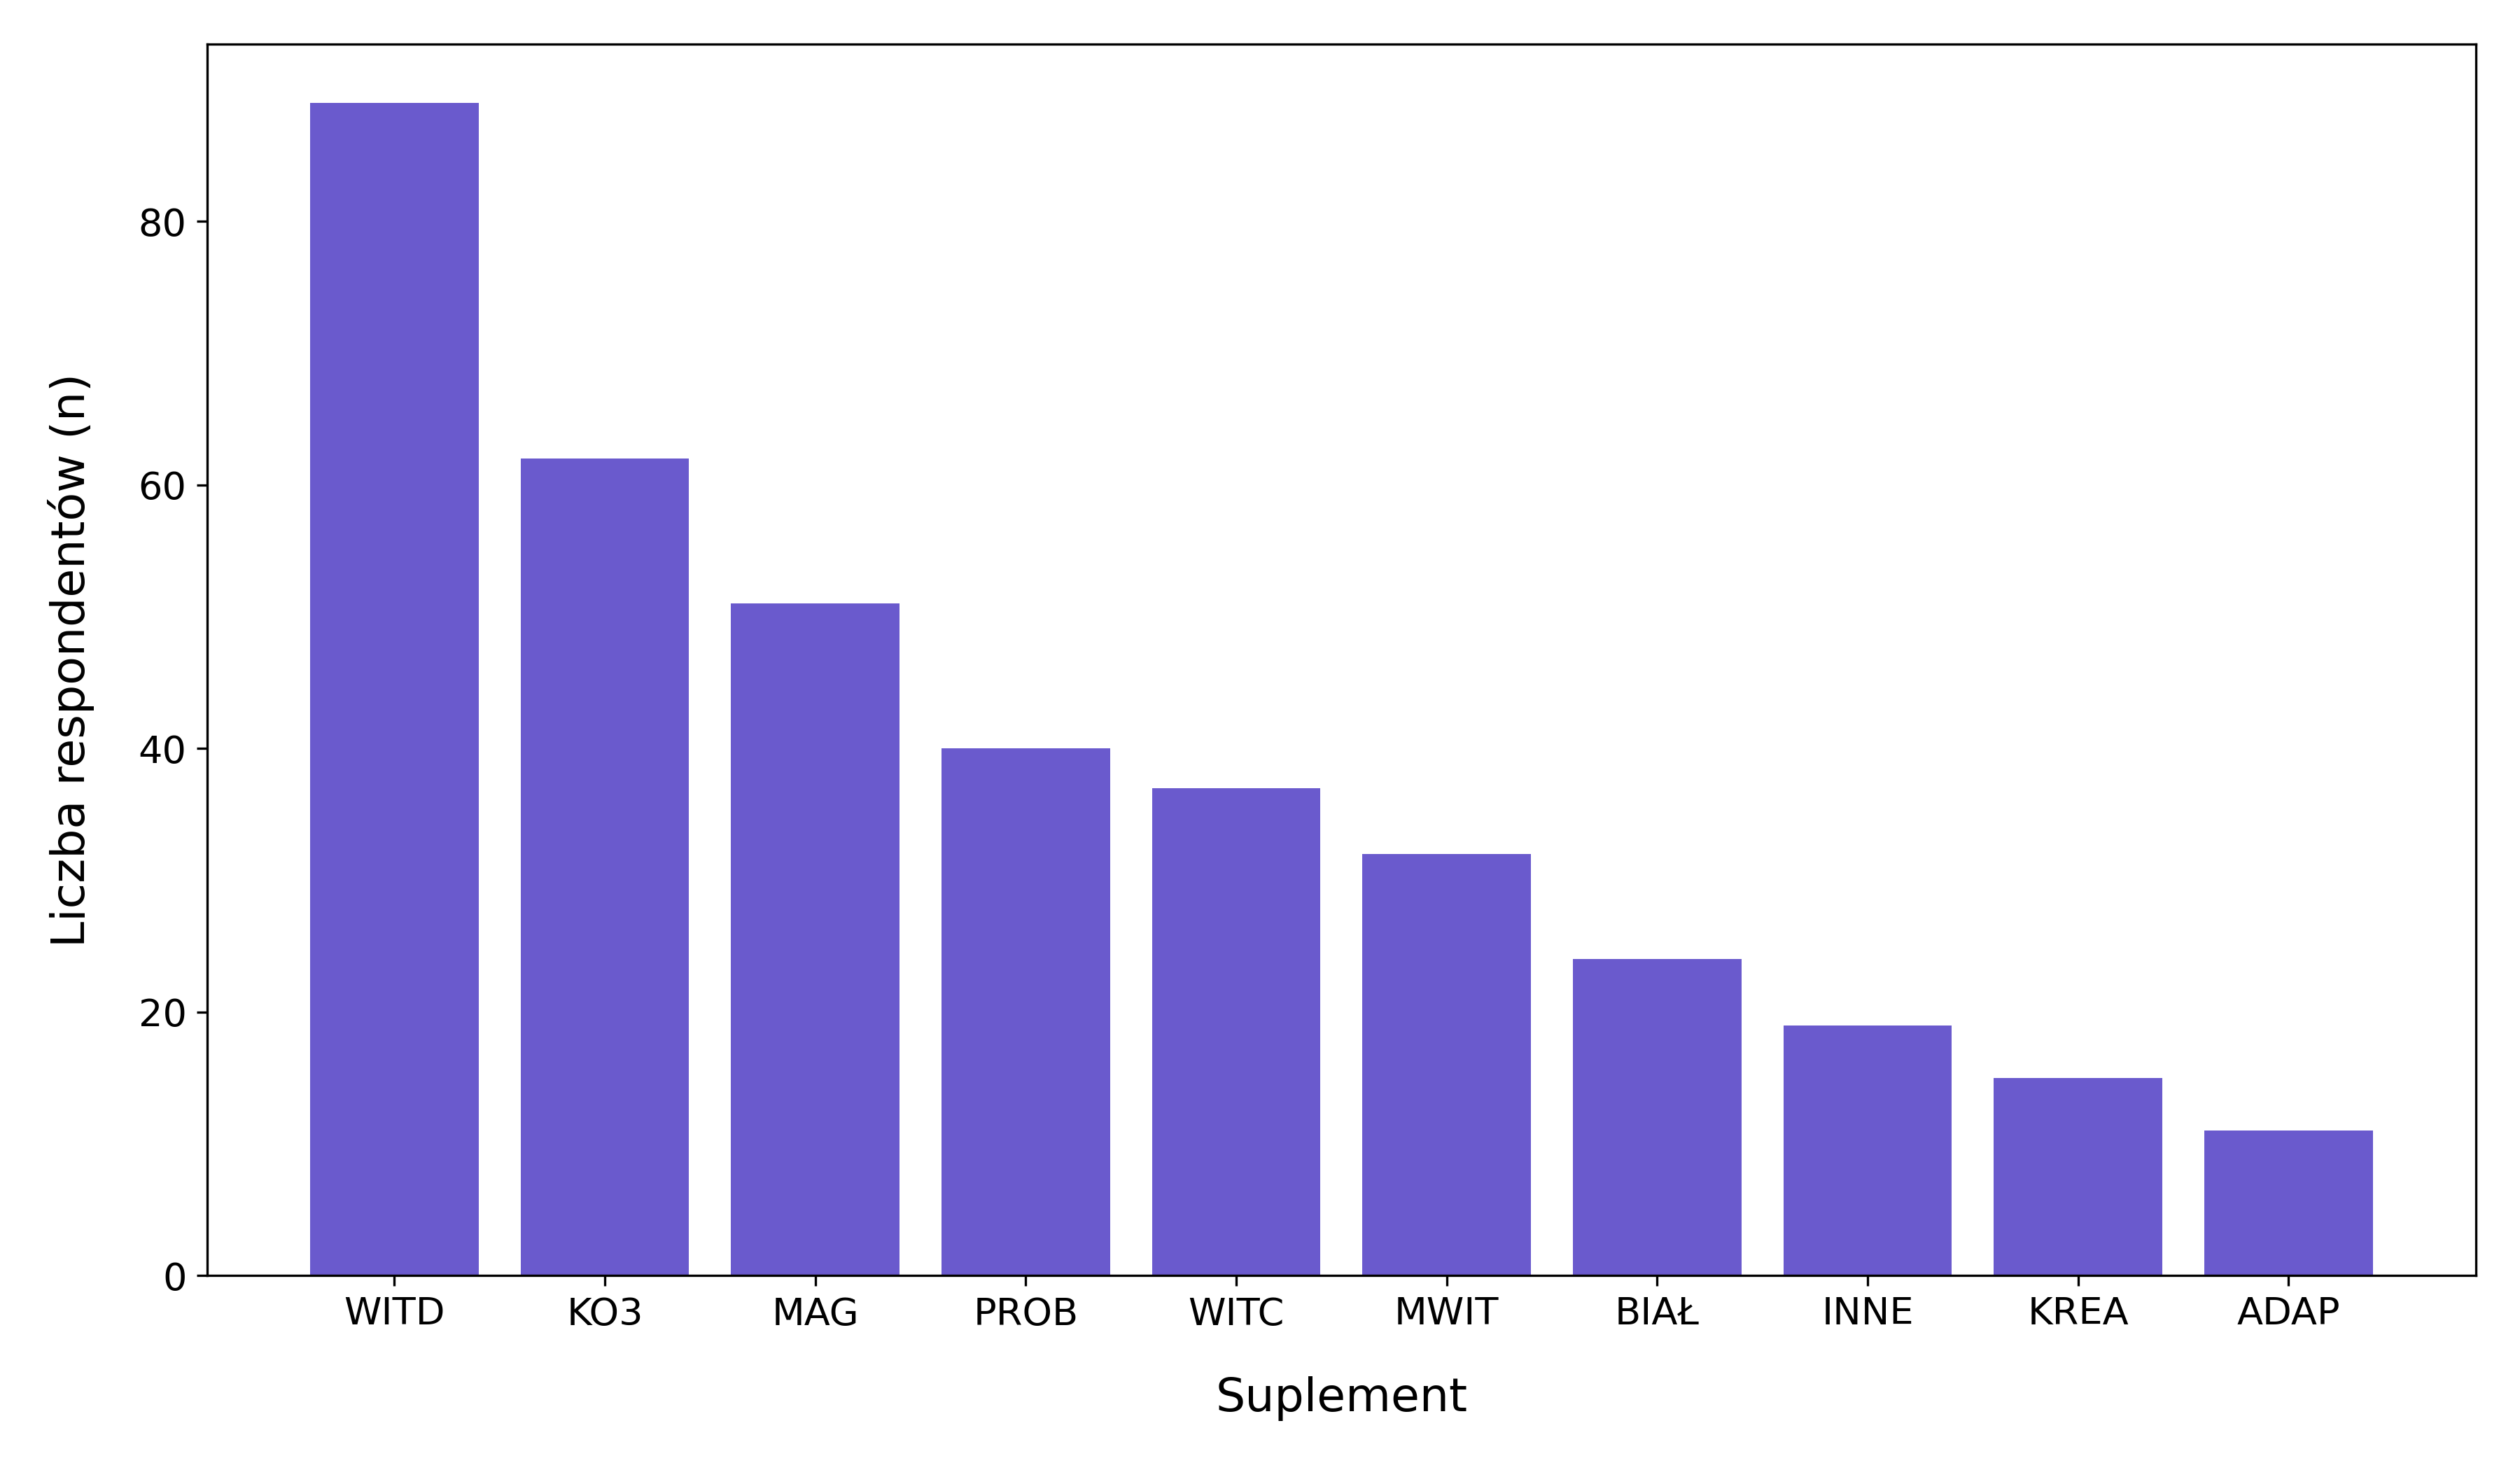
\includegraphics[width=\textwidth]{plots/rodzaje-suplementow.png}
    \centering
    \caption{Wykres słupkowy pokazujący rodzaje stosowanych suplementów w grupie badawczej. Zastosowane skróty: WITD - Witamina D, MAG - Magnez, WITC - Witamina C, MWIT - Multiwitaminy, KO3 - Kwasy omega-3, PROB - Probiotyki, KREA - Kreatyna, BIAŁ - Białko, ADAP - Adaptogeny (np. ashwagandha), INNE - Inne odpowiedzi.}

    \label{fig:rodz-stos-supl}
\end{figure}

% Statystyka
% Statystyka opisowa:
%     + n,
%     + %.

\subsection{Powody suplementacji}

% To również pytanie wielokrotnego wyboru. Procenty liczymy względem liczby osób stosujących suplementy.

% Tabela 6. Powody stosowania suplementów diety
% Powód stosowania, n, % osób stosujących suplementy
% Poprawa zdrowia
%   + Zapobieganie niedoborom
%   + Wzmocnienie odporności
%   + Poprawa wyglądu
%   + Zwiększenie energii
%   + Poprawa koncentracji
%   + Poprawa samopoczucia
%   + Inne

% Powody suplementacji

\begin{table}[h!]
    \centering
    \caption{Powody suplementacji}
    \label{tab:powody-supl}
    \begin{tabular}{|l|l|l|}
        \hline
        Powód stosowania & n  & \% respondentów \\
        \hline
        \hline
        Poprawa zdrowia & 68 & 70.1 \\
        \hline
        Wzmocnienie odporności & 66 & 68.04 \\
        \hline
        Zapobieganie niedoborom & 65 & 67.01 \\
        \hline
        Poprawa samopoczucia & 50 & 51.55 \\
        \hline
        Zwiększenie energii & 49 & 50.52 \\
        \hline
        Poprawa wyglądu (skóra, włosy, paznokcie) & 46 & 47.42 \\
        \hline
        Poprawa koncentracji & 44 & 45.36 \\
        \hline
        Inne odpowiedzi & 4  & 4.12 \\
        \hline
    \end{tabular}
\end{table}

\begin{figure}
    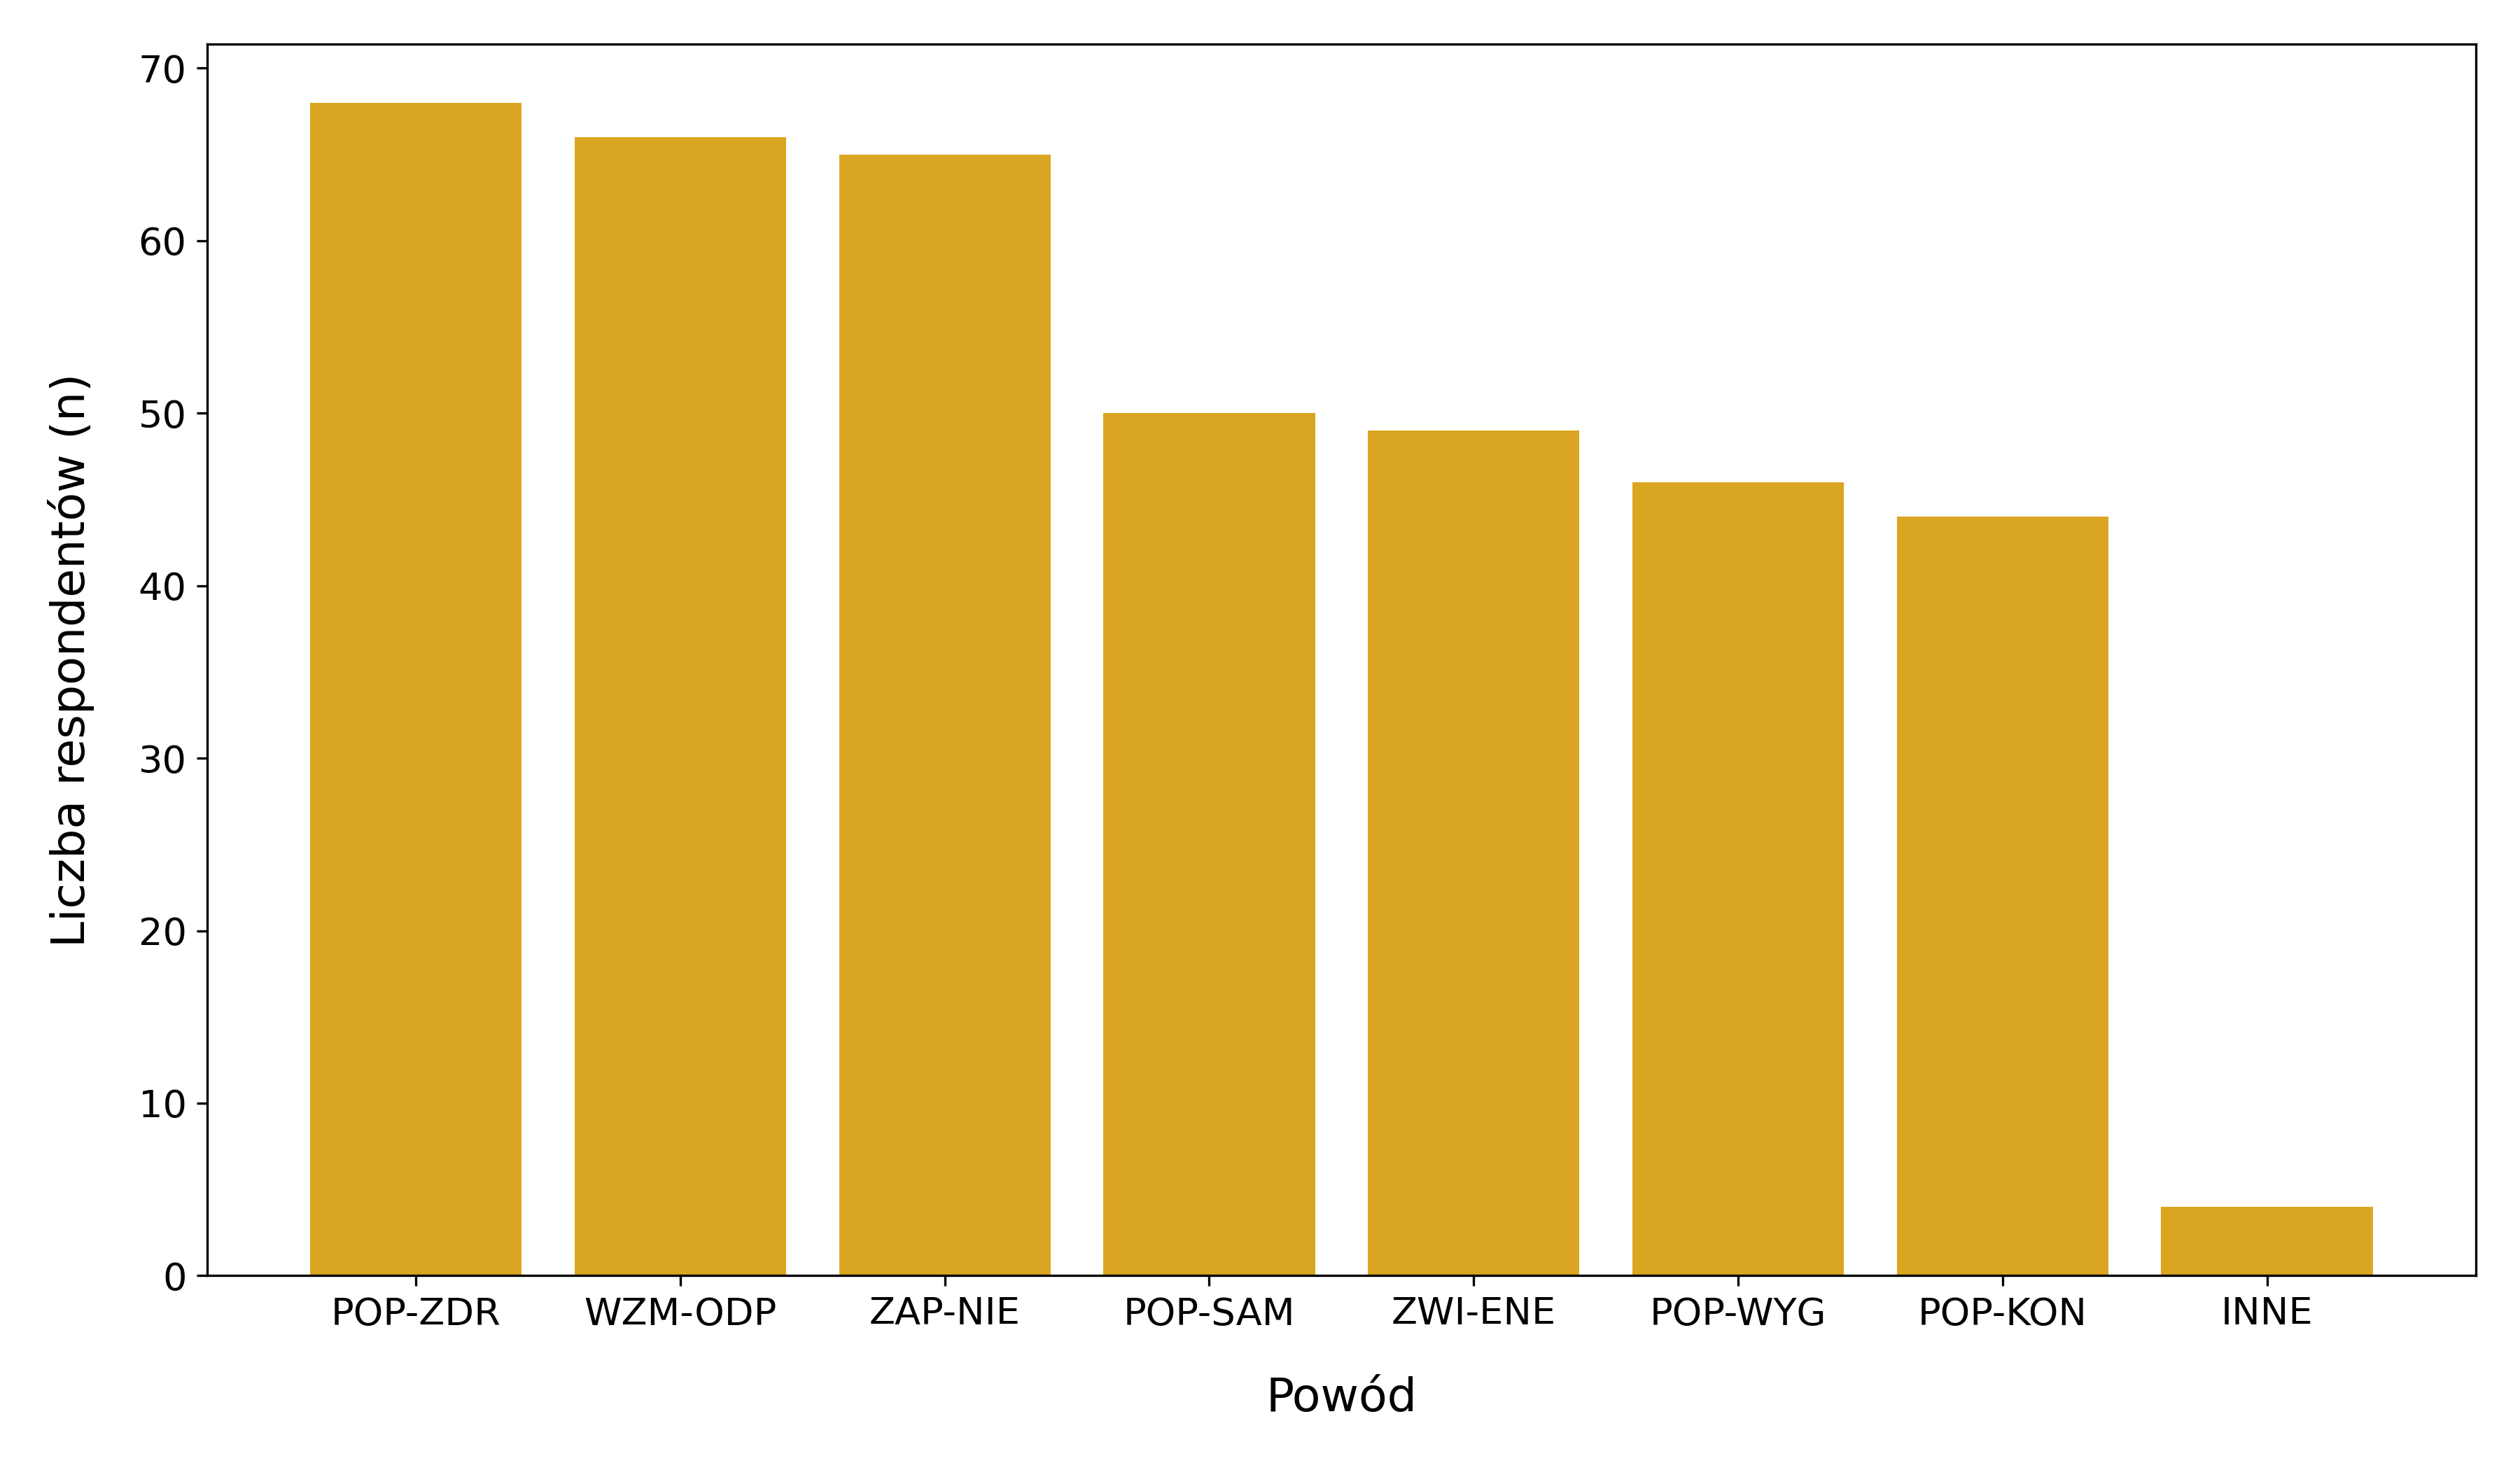
\includegraphics[width=\textwidth]{plots/powody-suplementacji.png}
    \centering
    \caption{Wykres słupkowy pokazujący powody suplementacji w grupie badawczej. Zastosowane skróty: POPZDR - Poprawa zdrowia, ZAPNIE - Zapobieganie niedoborom, WZMODP - Wzmocnienie odporności, POPWYG - Poprawa wyglądu (skóra włosy paznokcie), ZWIENE - Zwiększenie energii, POPKON - Poprawa koncentracji, POPSAM - Poprawa samopoczucia, INNE - Inne odpowiedzi.}
    \label{fig:powody-supl}
\end{figure}

% Wykres
% Poziomy wykres słupkowy - ranking powodów suplementacji.
% Statystyka
% Opisowo:
%     + n,
%     + %.

\subsection{Źródła wiedzy}

% Należy pokazać, skąd studenci czerpią wiedzę o suplementach.

% Źródła

\begin{table}[h!]
    \centering
    \caption{Źródła informacji}
    \label{tab:zrodla-info}
    \begin{tabular}{|l|l|l|}
        \hline
        Źródło & n  & \% respondentów \\
        \hline
        \hline
        Internet (artykuły, blogi) & 67 & 69.07 \\
        \hline
        Lekarz & 39 & 40.21 \\
        \hline
        Dietetyk & 37 & 38.14 \\
        \hline
        Media społecznościowe  & 31 & 31.96 \\
        \hline
        Znajomi/rodzina & 29 & 29.9 \\
        \hline
        Farmaceuta & 27 & 27.84 \\
        \hline
        Reklamy & 10 & 10.31 \\
        \hline
        Inne odpowiedzi & 10  & 10.31 \\
        \hline
    \end{tabular}
\end{table}

\begin{figure}
    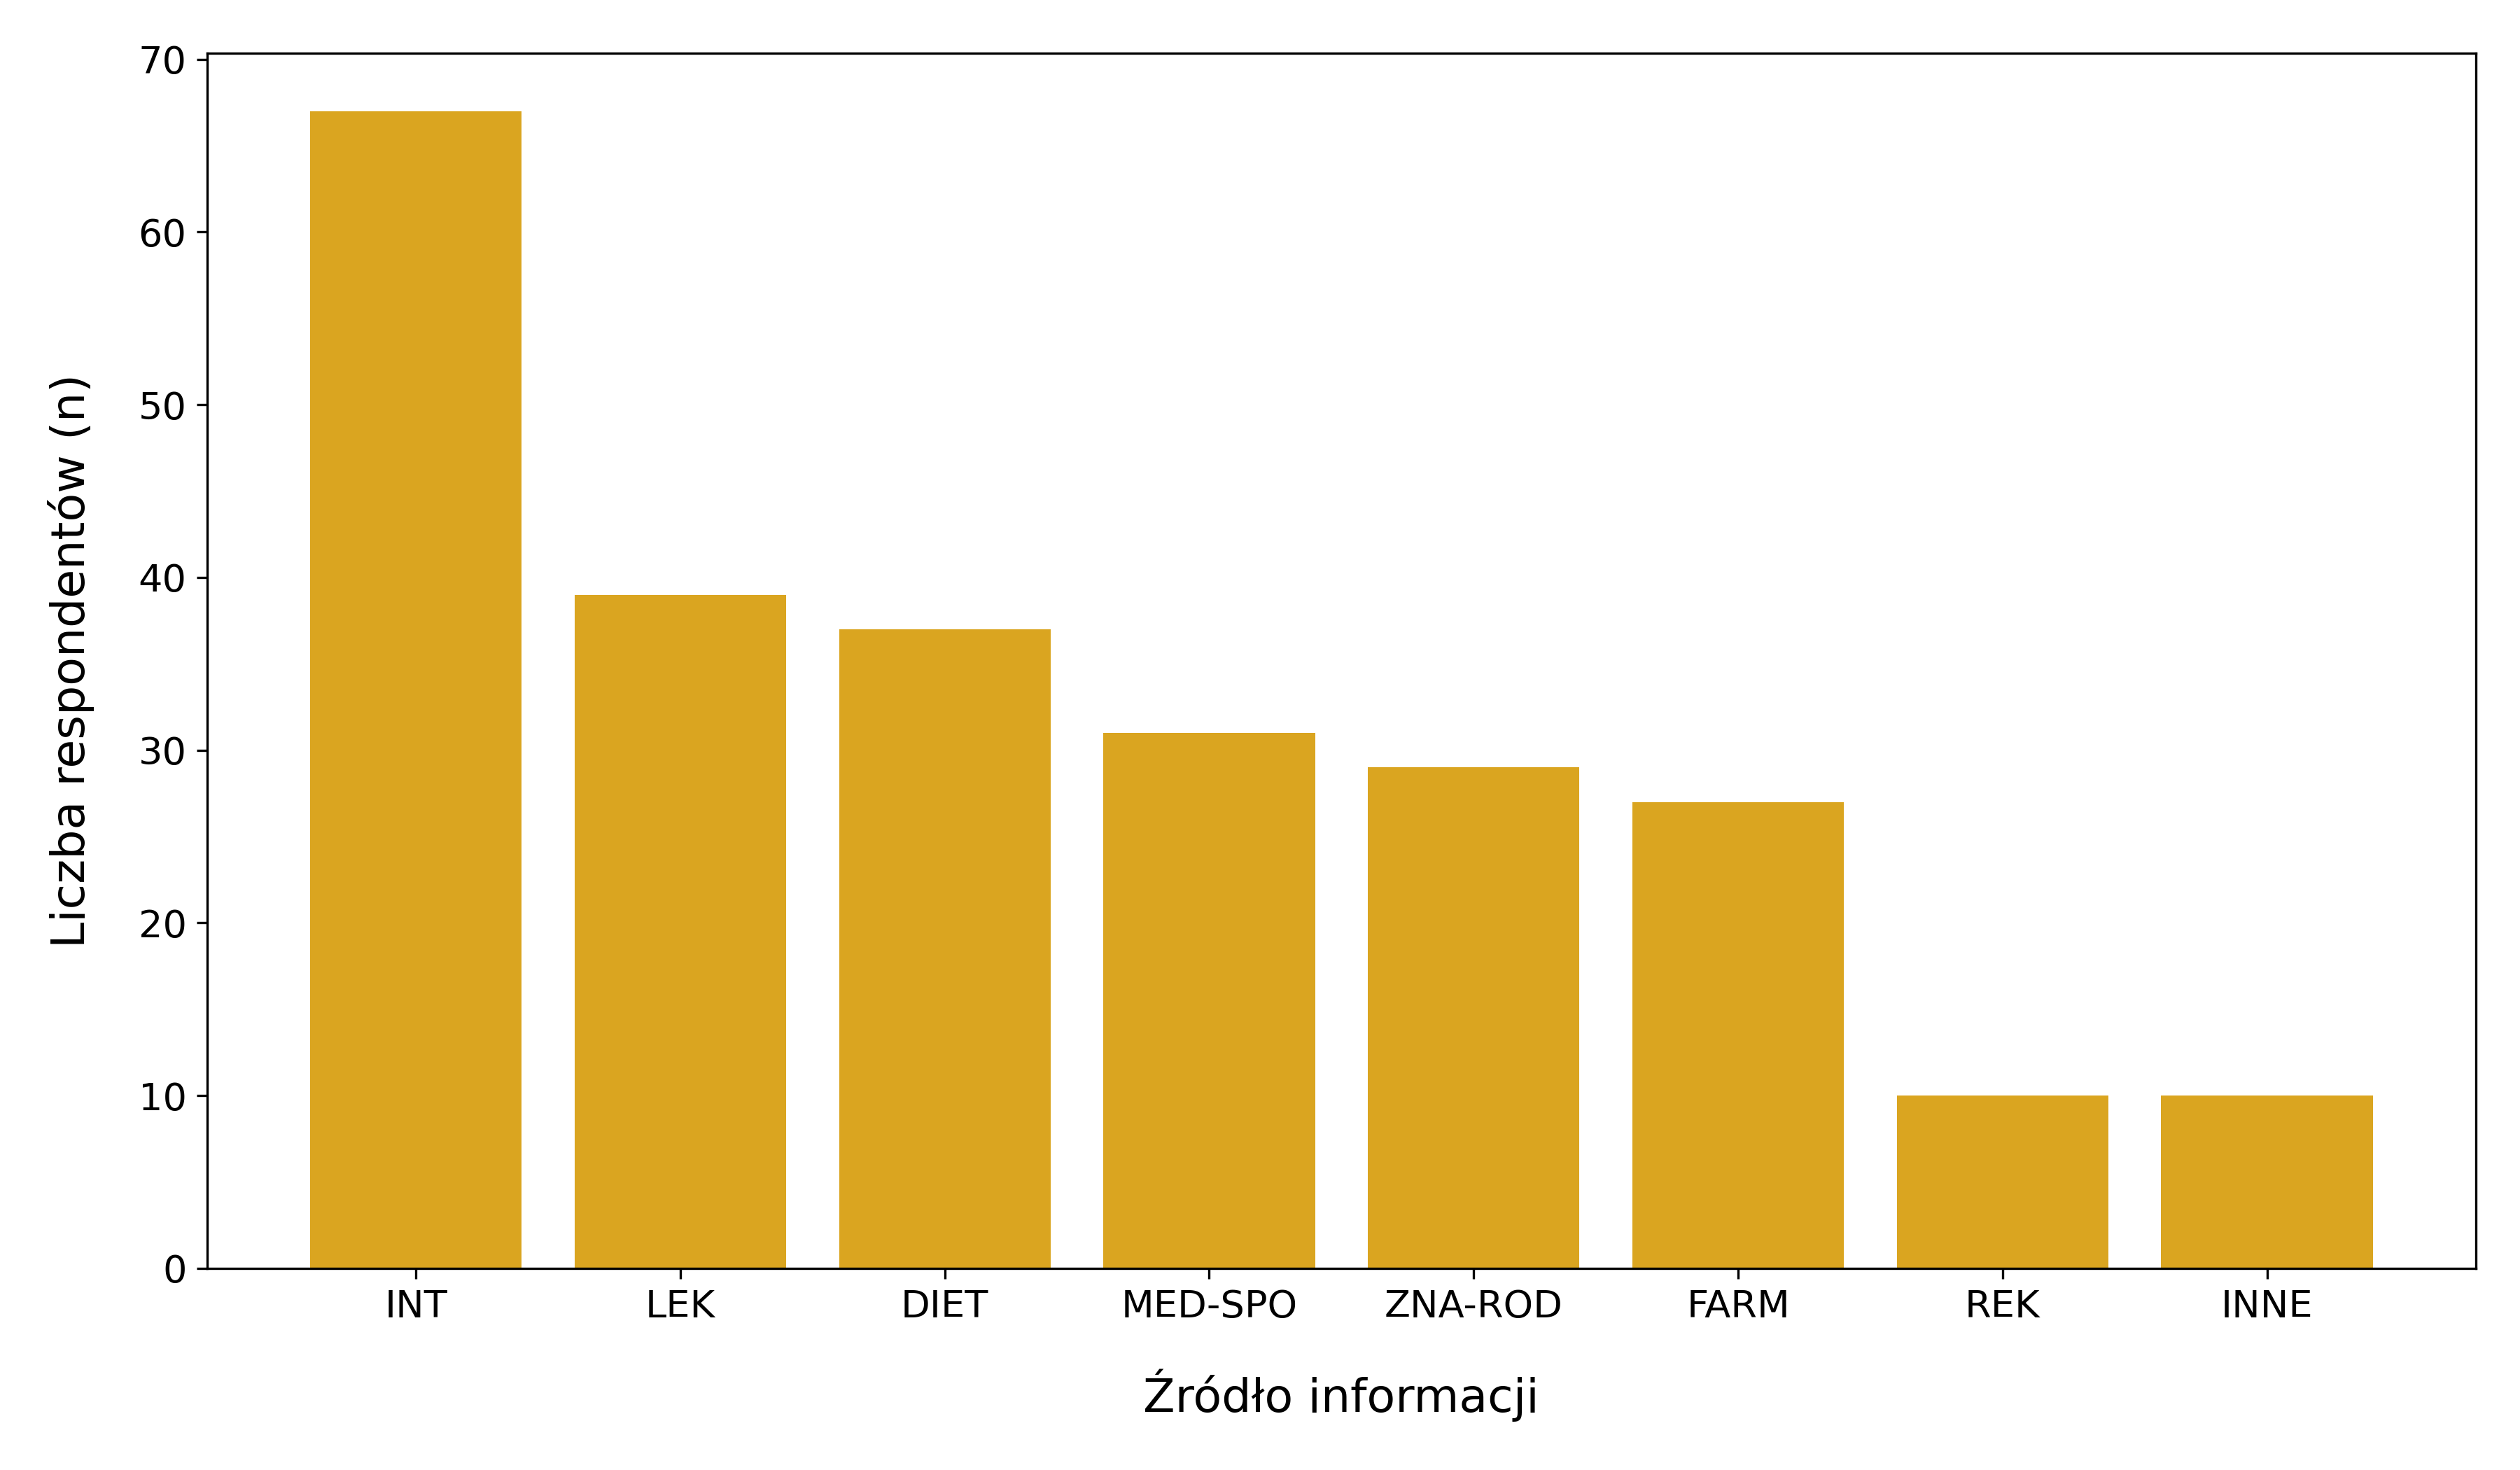
\includegraphics[width=\textwidth]{plots/zrodla-informacji.png}
    \centering
    \caption{Wykres pokazujący źródła informacji o suplementach w grupie badawczej. Zastosowane skróty: INT - Internet (artykuły, blogi), LEK - Lekarz, DIET - Dietetyk, MED-SPO - Media społecznościowe, ZNA-ROD - Znajomi/rodzina, FARM - Farmaceuta, REK - Reklamy, INNE - Inne odpowiedzi.}
    \label{fig:zrodla-info}
\end{figure}

% Wiarygodne źródła

\begin{table}[h!]
    \centering
    \caption{Wiarygodne źródła informacji. Zastosowane skróty: PROF - \enquote{Takie, którego polecenia nie wynikają z profitów jakie otrzymują}, FUNK - \enquote{Lekarze medycyny funkcjonalnej}, ZBR - \enquote{Portale zbierające wyniki badań lub też oponie specjalistów, ale wielu, żeby mozna było porównać podejścia, nie ufam jednemu lekarzowi, dietetykowi itp. ponieważ każdy mówi co innego}.}
    \label{tab:wiarygodne-zrodla}
    \begin{tabular}{|l|l|l|}
        \hline
        Źródło & n  & \% respondentów \\
        \hline
        \hline
        Lekarz & 67 & 69.07 \\
        \hline
        Naukowe portale internetowe & 39 & 40.21 \\
        \hline
        Instytucje zdrowia publicznego & 37 & 38.14 \\
        \hline
        Dietetyk & 31 & 31.96 \\
        \hline
        Farmaceuta & 29 & 29.9 \\
        \hline
        Badania naukowe & 27 & 27.84 \\
        \hline
        PROF & 10 & 10.31 \\
        \hline
        FUNK & 10  & 10.31 \\
        \hline
        ZBR & 10  & 10.31 \\
        \hline
    \end{tabular}
\end{table}

\begin{figure}
    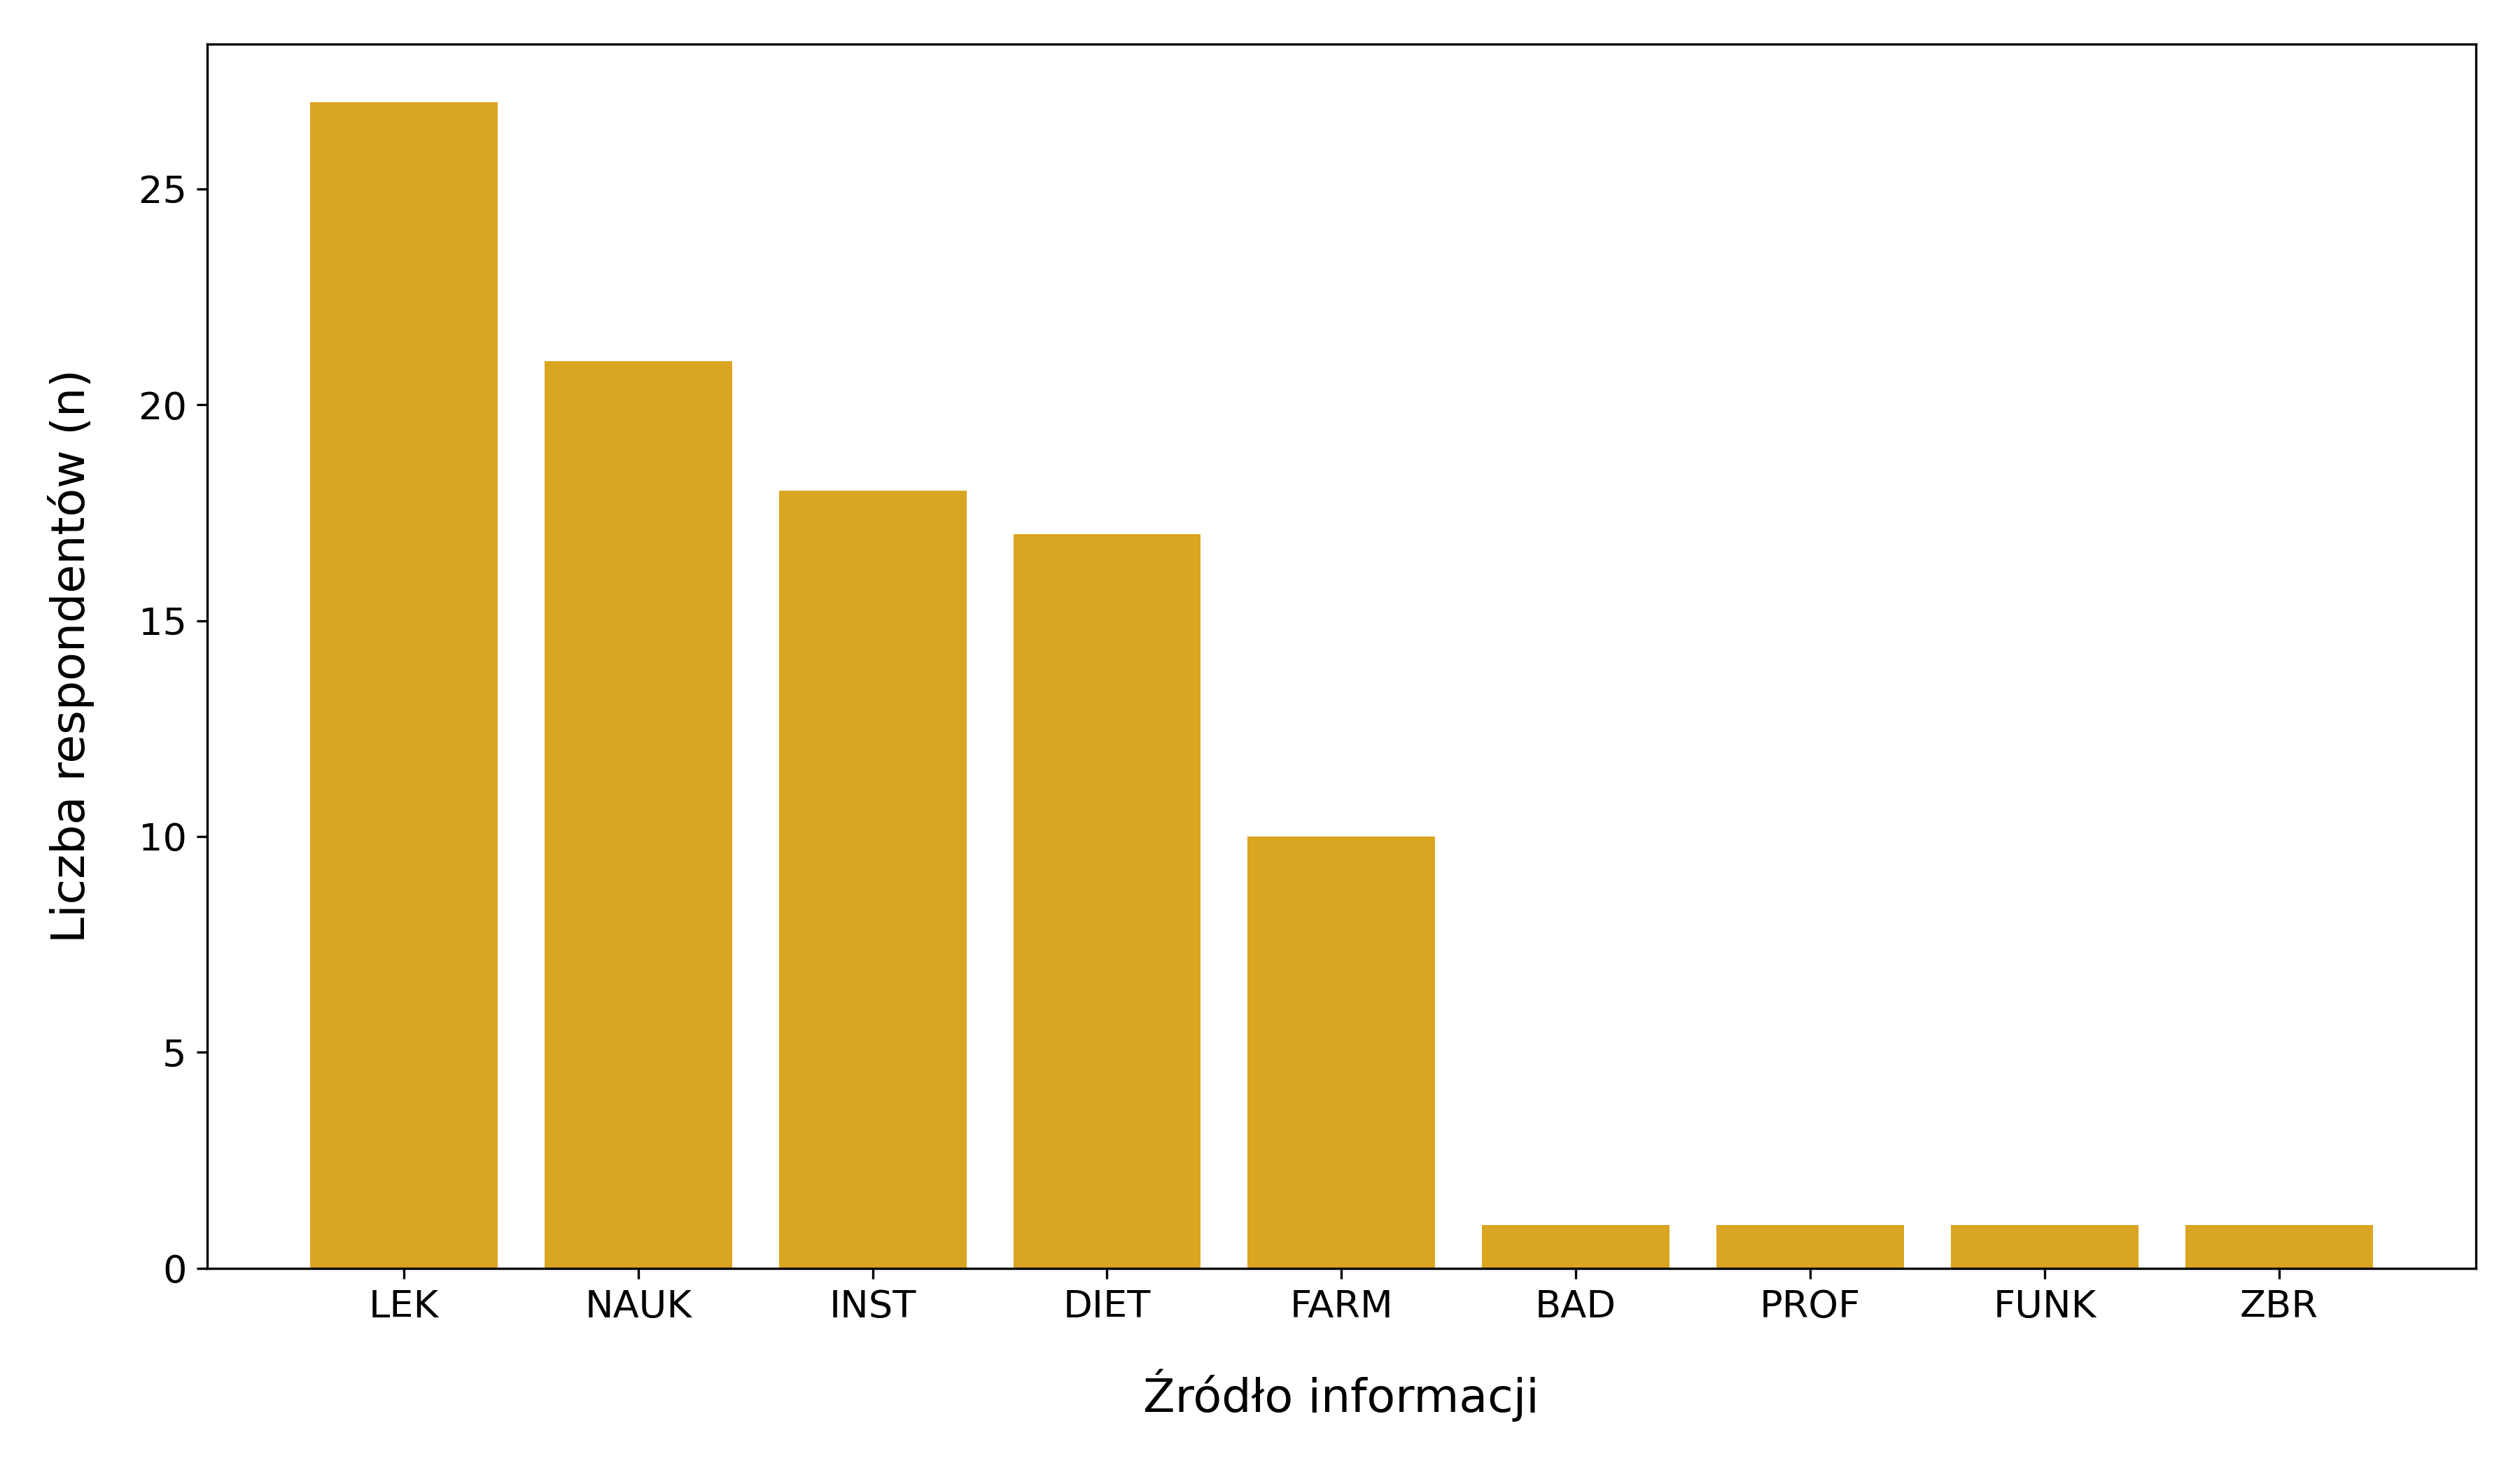
\includegraphics[width=\textwidth]{plots/wiarygodne-zrodla.png}
    \centering
    \caption{Wykres pokazujący zaufanie w różne źródła informacji o suplementach w grupie badawczej. Zastosowane skróty: LEK - Lekarz, NAUK - Naukowe portale internetowe, INST - Instytucje zdrowia publicznego, DIET - Dietetyk, FARM - Farmaceuta, BAD - Badania naukowe, PROF - \enquote{Takie, którego polecenia nie wynikają z profitów jakie otrzymują}, FUNK - \enquote{Lekarze medycyny funkcjonalnej}, ZBR - \enquote{Portale zbierające wyniki badań lub też oponie specjalistów, ale wielu, żeby mozna było porównać podejścia, nie ufam jednemu lekarzowi, dietetykowi itp. ponieważ każdy mówi co innego}.}
    \label{fig:wiarygodne-zrodla}
\end{figure}

% Preferowane formy edukacji

\begin{table}[h!]
    \centering
    \caption{Preferowane formy edukacji}
    \label{tab:formy}
    \begin{tabular}{|l|l|l|}
        \hline
        Forma & n  & \% respondentów \\
        \hline
        \hline
        Krótkie filmy edukacyjne & 53 & 54.64 \\
        \hline
        Artykuły popularnonaukowe & 45 & 46.39 \\
        \hline
        Warsztaty na uczelni & 39 & 40.21 \\
        \hline
        Infografiki & 32 & 32.99 \\
        \hline
        Konsultacje z farmaceutą & 32 & 32.99 \\
        \hline
        Posty na Instagramie/TikToku & 32 & 32.99 \\
        \hline
        Podcasty & 29 & 29.9 \\
        \hline
        Inne odpowiedzi & 5 & 5.15 \\
        \hline
    \end{tabular}
\end{table}

\begin{figure}
    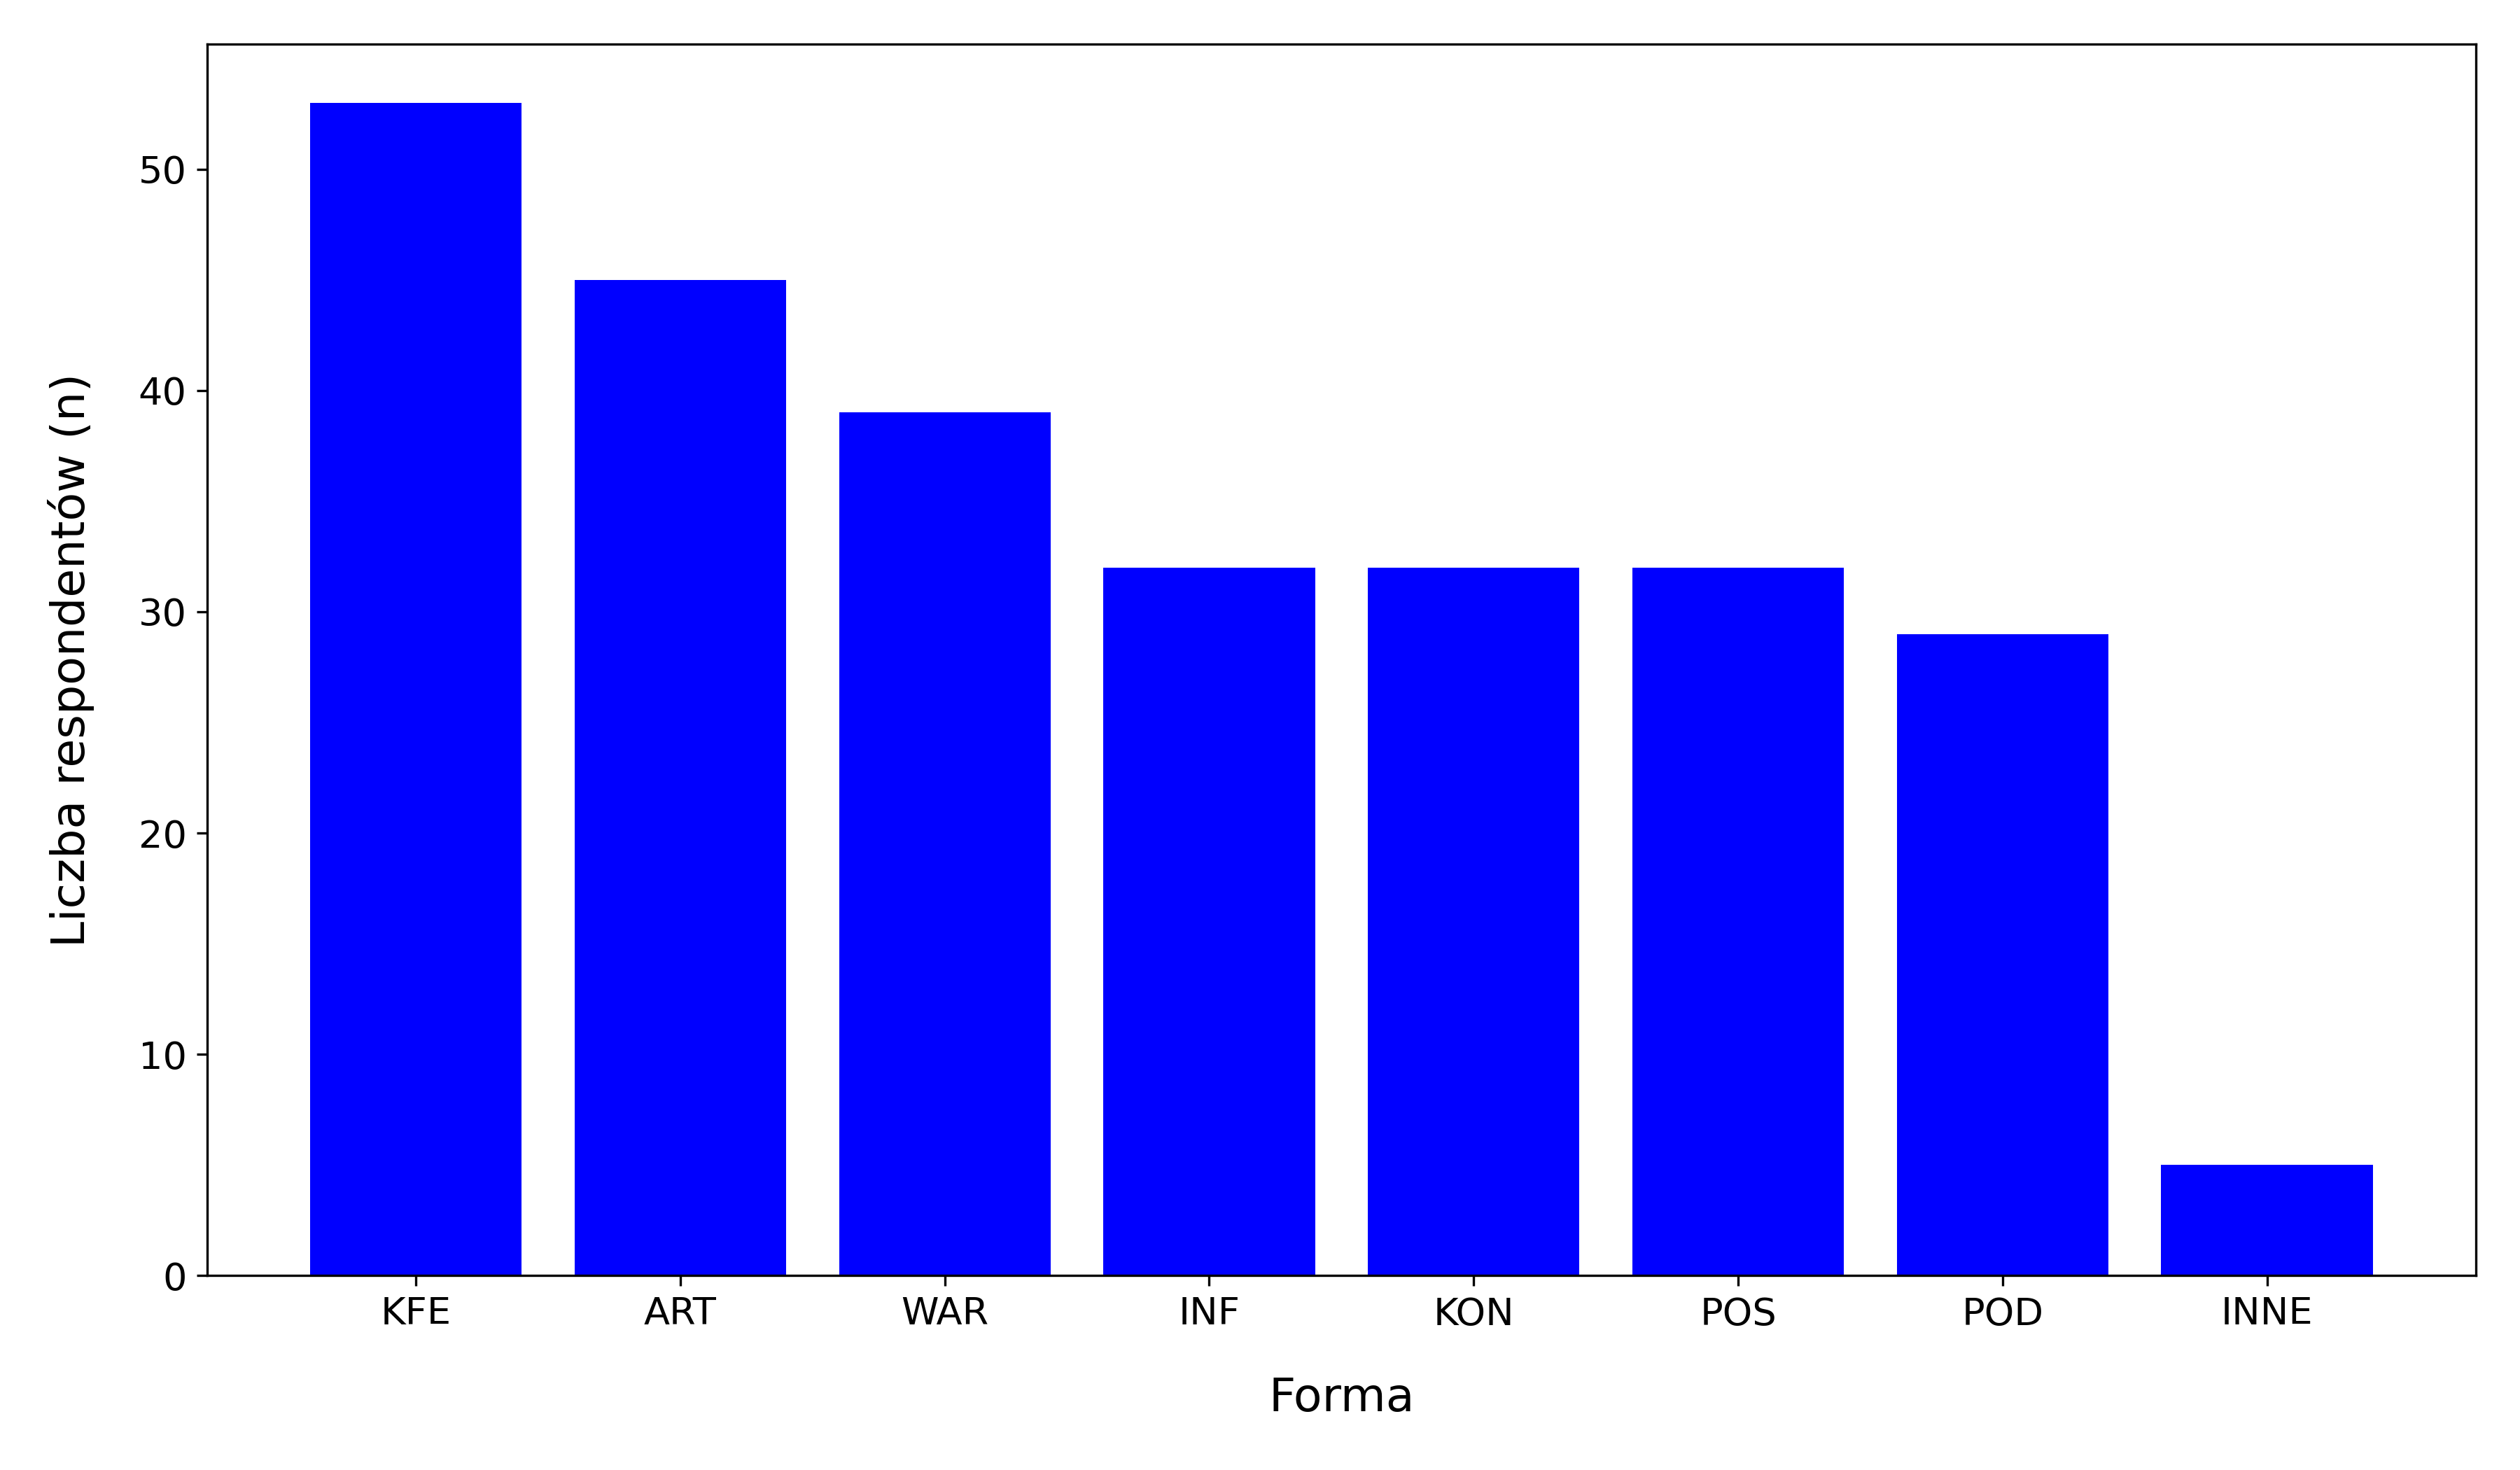
\includegraphics[width=\textwidth]{plots/preferowane-zrodla.png}
    \centering
    \caption{Wykres pokazujący preferowane formy edukacji o suplementach w grupie badawczej. Zastosowane skróty: KFE - Krótkie filmy edukacyjne, ART - Artykuły popularnonaukowe, WAR - Warsztaty na uczelni, INF - Infografiki, KON - Konsultacje z farmaceutą, POS - Posty na Instagramie/TikToku, POD - Podcasty, INNE - Inne odpowiedzi.}
    \label{fig:formy}
\end{figure}

% Tabela 7. Źródła informacji o suplementach diety
% Źródło informacji, n, %
%     + Internet
%     + Media społecznościowe
%     + Reklamy
%     + Lekarz
%     + Dietetyk
%     + Farmaceuta
%     + Znajomi/rodzina
%     + Inne
% Wykres
% Poziomy wykres słupkowy.


% Statystyka
% Opisowo:
%     + n,
%     + %.
% Można dodatkowo podzielić źródła na dwie grupy:
% Źródła profesjonalne
%     + lekarz,
%     + dietetyk,
%     + farmaceuta,
%     + instytucje zdrowia publicznego.
% Źródła nieprofesjonalne
%     + Internet,
%     + media społecznościowe,
%     + reklamy,
%     + znajomi/rodzina.

\subsection{Praktyki suplementacyjne}

% To bardzo ważny podrozdział, ponieważ pokazuje, czy suplementacja jest racjonalna.
% Należy uwzględnić pytania dotyczące:
%     1. przekraczania zalecanych dawek,
%     2. sprawdzania powielania składników,
%     3. wykonywania badań krwi przed suplementacją,
%     4. konsultowania suplementacji ze specjalistą.

% Tabela 8. Praktyki związane z bezpieczeństwem suplementacji
% Praktyka, Odpowiedź, n, %
% Przekraczanie zalecanej dawki, Nigdy / Czasami / Często
% Sprawdzanie powielania składników, Tak / Czasami / Nie
% Badania krwi przed suplementacją, Tak / Częściowo / Nie
% Konsultacja ze specjalistą, Lekarz / Dietetyk / Farmaceuta / Nie

% Statystyka Opisowo:
%     + n,
%     + %.
% Dodatkowo można utworzyć indeks prawidłowych praktyk suplementacyjnych.

\subsection{Indeks prawidłowych praktyk suplementacyjnych}

% Proponuję utworzyć prosty wskaźnik 0–4 punkty.

% Punktacja
% 1. Przekraczanie dawek
%     + nigdy nie przekracza dawki: 1 punkt,
%     + czasami/często przekracza: 0 punktów.
% 2. Sprawdzanie powielania składników
%     + zawsze sprawdza: 1 punkt,
%     + czasami/nie sprawdza: 0 punktów.
% 3. Badania krwi przed suplementacją
%     + tak, wykonuje badania: 1 punkt,
%     + tylko przy niektórych preparatach / nie: 0 punktów.
% 4. Konsultacja ze specjalistą
%     + konsultuje z lekarzem, dietetykiem lub farmaceutą: 1 punkt,
%     + nie konsultuje: 0 punktów.
% Zakres wyniku
% Od 0 do 4 punktów.
% Im wyższy wynik, tym bardziej prawidłowe praktyki suplementacyjne.

% Tabela 9. Indeks prawidłowych praktyk suplementacyjnych
% Wynik indeksu, n, %
%     + 0 pkt
%     + 1 pkt
%     + 2 pkt
%     + 3 pkt
%     + 4 pkt
% Można też stworzyć kategorie
%     + 0–1 pkt: niska prawidłowość praktyk,
%     + 2 pkt: umiarkowana prawidłowość praktyk,
%     + 3–4 pkt: wysoka prawidłowość praktyk.

% Statystyka
% Dla indeksu praktyk należy podać:
%     + średnią,
%     + odchylenie standardowe,
%     + medianę,
%     + kwartyle Q1–Q3,
%     + minimum,
%     + maksimum.
% Ponieważ indeks ma mały zakres i charakter porządkowy, w analizach zależności najlepiej stosować testy nieparametryczne.

\subsection{Samoocena wiedzy o suplementach}

% W ankiecie są trzy pytania w skali 1–5:
%     1. ogólna wiedza o suplementach,
%     2. wiedza o bezpieczeństwie suplementacji,
%     3. wiedza o interakcjach suplementów z lekami.
% Tabela 10. Samoocena wiedzy respondentów
% Zmienna, Średnia, SD, Mediana, Q1–Q3, Min–Max
%     + Ogólna wiedza
%     + Wiedza o bezpieczeństwie
%     + Wiedza o interakcjach

% Wykres
% Najlepszy będzie wykres pudełkowy dla trzech zmiennych.

% Statystyka
% Ponieważ skala 1–5 jest skalą porządkową, należy podać:
%     + medianę,
%     + kwartyle,
%     + ewentualnie średnią i SD pomocniczo.
% Do porównań między grupami:
%     + dwie grupy: test U Manna–Whitneya,
%     + więcej niż dwie grupy: test Kruskala–Wallisa,
%     + zależności między skalami: korelacja Spearmana.

\subsection{Obiektywny poziom wiedzy - indeks wiedzy}

% Należy stworzyć indeks wiedzy na podstawie pytań testowych.
% Pytania punktowane
% 1. Suplement diety to:
% o. poprawna odpowiedź: środek spożywczy uzupełniający dietę.
% 2. Czy suplementy muszą przechodzić badania kliniczne przed wprowadzeniem na rynek?
% o. poprawna odpowiedź: nie.
% 3. Nadmierne spożycie witaminy D może prowadzić do:
% o. poprawna odpowiedź: uszkodzenia nerek.
% 4. Kto odpowiada za bezpieczeństwo suplementów diety?
% o. poprawna odpowiedź: producent.
% 5. Czy suplementy mogą wchodzić w interakcje z lekami?
% o. poprawna odpowiedź: tak.
% 6. Czy suplementy mogą zawierać składniki w ilościach przekraczających zapotrzebowanie?
% o. poprawna odpowiedź: tak.

% Punktacja
% Za każdą poprawną odpowiedź: 1 punkt.
% Za odpowiedź błędną lub „nie wiem”: 0 punktów.
% Zakres indeksu: 0–6 punktów.

% Tabela 11. Poprawność odpowiedzi na pytania wiedzy
% Pytanie, Poprawna opowiedź, n poprawnych, % poprawnych

% Tabela 12. Indeks wiedzy o suplementach
% Wynik indeksu, n, %
%     + 0 pkt
%     + 1 pkt
%     + 2 pkt
%     + 3 pkt
%     + 4 pkt
%     + 5 pkt
%     + 6 pkt

% Kategorie wiedzy
% Proponuję podział:
%     + 0–2 pkt: niski poziom wiedzy,
%     + 3–4 pkt: umiarkowany poziom wiedzy,
%     + 5–6 pkt: wysoki poziom wiedzy.

% Tabela 13. Kategorie poziomu wiedzy
% Poziom wiedzy, n, %
%     + Niski
%     + Umiarkowany
%     + Wysoki

% Wykres
% Wykres słupkowy pokazujący rozkład kategorii wiedzy.

% Statystyka
% Dla indeksu wiedzy należy podać:
%    + średnią,
%    + SD,
%    + medianę,
%    + Q1–Q3,
%    + minimum,
%    + maksimum.
% Ponieważ indeks ma zakres 0–6, w dalszych analizach najlepiej traktować go jako zmienną porządkową i stosować testy nieparametryczne.


\subsection{Analiza zależności}

\subsubsection{Czy stosowanie suplementów zależy od płci?}

\subsubsection{Czy stosowanie suplementów zależy od wieku?}

\subsubsection{Czy stosowanie suplementów zależy od aktywności fizycznej?}

\subsubsection{Czy poziom wiedzy różni się między osobami stosującymi i niestosującymi suplementy?}

\subsubsection{Czy poziom wiedzy wiąże się z konsultowaniem suplementacji ze specjalistą?}

\subsubsection{Czy poziom wiedzy wiąże się z wykonywaniem badań krwi przed suplementacją?}

\subsubsection{Czy poziom wiedzy wiąże się ze sprawdzaniem powielania składników?}

\subsubsection{Czy poziom wiedzy wiąże się z przekraczaniem zalecanych dawek?}

\subsubsection{Zależność między wiedzą deklarowaną a rzeczywistą}

\subsubsection{Czy osoby korzystające z profesjonalnych źródeł informacji mają wyższy poziom wiedzy?}

\subsubsection{Zależność między indeksem wiedzy a indeksem prawidłowych praktyk}


\subsection{Preferowane formy edukacji}

\subsection{Najbardziej wiarygodne źródła informacji}

\subsection{Zbiorcza tabela analiz statystycznych}


\section{Dyskusja}\label{Dyskusja}

% Dyskusja

Celem niniejszej pracy była analiza postaw, wiedzy oraz praktyk studentów w zakresie stosowania suplementów diety. Uzyskane wyniki wskazują na niezwykle wysoką powszechność tego zjawiska w badanej grupie – aż 90,7\% respondentów zadeklarowało aktualne przyjmowanie preparatów uzupełniających dietę. Wynik ten jest znacząco wyższy niż odnotowany w badaniu Sicińskiej i wsp. (2022) na Uniwersytecie Warszawskim (41\%) czy w badaniach studentów w Chorwacji (30,5\%) \cite{diet-lifestyle, croatia-knowledge-and-use}. Bliższy jest natomiast danym z Arabii Saudyjskiej (76,6\%) czy Bejrutu (68\%) \cite{alfawaz2017prevalence, pharmacist-knowledge-and-use}. Tak wysoki odsetek w badaniu własnym wynika prawdopodobnie ze specyfiki grupy badawczej, w której dominowali studenci psychologii i dietetyki (łącznie ponad 72\%), co zazwyczaj wiąże się z większym zainteresowaniem zdrowiem, profilaktyką oraz dobrostanem psychofizycznym.

W literaturze przedmiotu płeć biologiczna jest wskazywana jako jeden z najsilniejszych predyktorów stosowania suplementów. Badania Sicińskiej (2022) czy Vidovica (2022) sugerują, że mężczyźni sięgają po suplementy znacznie rzadziej niż kobiety (o ok. 38\%) \cite{sicinska2022dietary, vidovic2022dietary}. Co ciekawe, badania własne nie potwierdziły tej zależności ($p = 0,36$). Nie wykazano statystycznie istotnych różnic w częstości suplementacji między kobietami (88,9\%) a mężczyznami (100,0\%). Może to świadczyć o zacieraniu się różnic międzypłciowych w grupach o podobnym profilu wykształcenia (studenci akademicy) i wysokich zainteresowaniach prozdrowotnych, choć interpretację tę należy prowadzić ostrożnie ze względu na dużą dysproporcję liczebną płci w badanej próbie (84,1\% kobiet vs 15,9\% mężczyzn), co mogło ograniczyć moc testu statystycznego.

Podobny brak istotności odnotowano w przypadku wieku ($p = 0,54$) oraz poziomu aktywności fizycznej ($p = 0,17$). Choć we wszystkich podgrupach większość osób stosowała suplementy, to brak związku z aktywnością fizyczną stoi w lekkiej sprzeczności z częścią literatury (np. \cite{diet-lifestyle}), gdzie intensywny styl życia i sport mocno determinowały suplementację. W badanej grupie niska frekwencja stosowania typowych odżywek sportowych, takich jak białko (24,7\%) czy kreatyna (15,4\%), koreluje z faktem, że większość badanych (33,6\%) podejmowała aktywność rzadziej niż raz w tygodniu, a dominującą część próby stanowiły kobiety, które według literatury rzadziej wybierają preparaty ukierunkowane na budowanie masy mięśniowej \cite{vidovic2022dietary, radwan2019prevalence}.

Dominującym preparatem w badanej grupie była witamina D (81,4\%), co jest w pełni uzasadnione szeroką kampanią edukacyjną w Polsce dotyczącą powszechnych niedoborów tego składnika w naszej strefie klimatycznej. Na kolejnych miejscach znalazły się kwasy omega-3 (60,8\%) oraz magnez (49,4\%). Wyniki te różnią się od danych z USA czy Jordanii, gdzie studenci najczęściej wybierają ogólne preparaty multiwitaminowe i multimineralne \cite{lieberman2015patterns, knowledge-and-use}.

Główną motywacją badanych była chęć poprawy zdrowia (70,1\%), wzmocnienia odporności (68,04\%) oraz zapobiegania niedoborom (67,01\%). Koresponduje to z trendami światowymi opisywanymi przez Sundgota-Borgen i wsp. (2022) oraz badaniami z Bejrutu, gdzie motywacje zdrowotne i profilaktyczne wysuwały się na pierwszy plan \cite{sundgot2022explanations, pharmacist-knowledge-and-use}. Warto zauważyć, że blisko połowa respondentów (47,42\%) wskazała również na powody estetyczne (poprawa wyglądu skóry, włosów i paznokci), co idealnie wpisuje się w doniesienia Lawanda i współpracowników (2023) o rosnącym znaczeniu aspektów kosmetycznych w decyzjach o suplementacji wśród młodych dorosłych \cite{lawand2023assessment}.

Głównym źródłem informacji o suplementach diety dla badanych studentów pozostał internet (69,07\%), co jest zjawiskiem powszechnym i zgodnym z badaniami globalnymi, gdzie media cyfrowe osiągają wskaźniki rzędu 38\%–40\% \cite{kobayashi2017prevalence, chiba2020educational}. Niepokojący w literaturze jest fakt, że rzadko towarzyszą temu konsultacje ze specjalistami \cite{croatia-knowledge-and-use}. W badaniach własnych odsetek konsultacji z lekarzem (40,21\%) i dietetykiem (38,14\%) okazał się relatywnie wysoki na tle innych krajów, co ponownie można przypisać obecności studentów dietetyki w próbie.

Zauważalny jest jednak dualizm postaw: lekarz jest uznawany przez studentów za najbardziej wiarygodne źródło informacji (69,07\%), a naukowe portale internetowe zajmują drugie miejsce (40,21\%). Mimo tak wysokiego zaufania deklaratywnego, w praktyce aż 47,42\% respondentów wskazało, że w ogóle nie konsultuje swojej suplementacji ze specjalistą, podejmując decyzje autonomicznie. Zjawisko to potwierdza teorię Steele i Senekal (2005) o silnym wpływie marketingu bezpośredniego i subiektywnego poczucia bezpieczeństwa stosowania tych produktów \cite{steele2005dietary}.

Kluczowym i najbardziej intrygującym wnioskiem z przeprowadzonej analizy statystycznej jest brak przełożenia wiedzy na realne praktyki bezpiecznej suplementacji. Z jednej strony, studenci wykazali się dobrą zdolnością do samokrytyki – ich samoocena wiedzy umiarkowanie, ale istotnie korelowała z rzeczywistym wynikiem testowym (dla ogólnej wiedzy $\rho = 0,47$, dla interakcji $\rho = 0,54$, przy $p < 0,001$). Średni obiektywny poziom wiedzy wyniósł 3,76 na 6 punktów, a blisko 40\% badanych osiągnęło wysoki próg punktowy. Wynik ten jest lepszy niż w badaniach Homana (2018) czy Elsahoryi (2023), gdzie studenci odpowiadali poprawnie na mniej niż połowę pytań \cite{homan2018dietary, elsahoryi2023prevalence}.

Z drugiej strony, analiza wykazała brak istotnej korelacji między indeksem wiedzy a indeksem prawidłowych praktyk suplementacyjnych ($\rho = 0,15$; $p = 0,11$). Co więcej:

\begin{itemize}
    \item Wyższy poziom wiedzy nie różnicował osób pod kątem wykonywania badań krwi przed rozpoczęciem suplementacji ($p = 0,19$).
    \item Wiedza nie wpływała na to, czy studenci konsultowali się ze specjalistą ($p = 0,57$).
    \item Zależność między wiedzą a przekraczaniem zalecanych dawek znalazła się na granicy istotności statystycznej ($p = 0,052$), co sugeruje jedynie słaby trend, według którego wyższa świadomość może (choć nie musi) chronić przed dawkowaniem niezgodnym z zaleceniami.
\end{itemize}

Jedynym obszarem, w którym wiedza odegrała skrajnie istotną rolę, było sprawdzanie powielania składników w przyjmowanych preparatach ($p = 0,0001$). Średnia wiedzy w grupie sprawdzającej skład wyniosła 4,9 pkt. względem 3,6 pkt. w grupie niesprawdzającej.

Ten stan rzeczy obnaża wyraźną lukę behawioralną: studenci posiadający wiedzę teoretyczną potrafią zastosować ją do czytania etykiet i unikania dublowania dawek (co jest czynnością prostą, analityczną), jednak ta sama wiedza nie motywuje ich do wdrażania głębszych procedur bezpieczeństwa, takich jak diagnostyka laboratoryjna czy profesjonalna konsultacja medyczna. Wpisuje się to w mity opisywane przez Chibę i wsp. (2020), zgodnie z którymi młode osoby, nawet dobrze wyedukowane, podświadomie traktują suplementy jako „całkowicie bezpieczną żywność naturalną”, przez co rezygnują z rygorystycznych środków ostrożności \cite{chiba2020educational}. Ogólny indeks praktyk w badaniu własnym okazał się niski u aż 41,24\% respondentów, co potwierdza, że wiedza teoretyczna nie jest wystarczającym czynnikiem gwarantującym bezpieczeństwo zdrowotne.

Głównym ograniczeniem niniejszego badania jest brak pełnej reprezentatywności akademickiej – silne skrzywienie próby w stronę kobiet oraz studentów kierunków o profilu medycznym i humanistycznym (dietetyka, psychologia) utrudnia generalizację wyników na całą populację studencką (np. kierunki techniczne czy ścisłe). Ponadto mała liczebność grupy niestosującej suplementów ($n = 10$) ograniczyła możliwości porównawcze w niektórych testach.

Mimo to, uzyskane dane wyraźnie definiują potrzeby edukacyjne młodych dorosłych. Prawie połowa studentów (50,12\%) nie wiedziała o braku konieczności przeprowadzania badań klinicznych dla suplementów diety przed wprowadzeniem ich na rynek, co potwierdza tezę Homana (2018) o nieznajomości podstaw prawnych i regulacyjnych \cite{homan2018dietary}. Projektując przyszłe interwencje edukacyjne, należy porzucić suche wykłady akademickie na rzecz form preferowanych przez samych studentów – ponad połowa (54,64\%) wskazała krótkie filmy edukacyjne, a duża część artykuły popularnonaukowe (46,39\%) i warsztaty praktyczne (40,21\%). Edukacja ta powinna kłaść nacisk nie tyle na biochemiczną teorię witamin, ile na kształtowanie prawidłowych nawyków behawioralnych (konieczność badań krwi, ryzyko samowolnej suplementacji).


\section{Wnioski}\label{Wnioski}

Przedstawione poniżej wnioski końcowe stanowią bezpośrednie podsumowanie realizacji celu głównego oraz celów szczegółowych pracy, a także zawierają odpowiedź na pytanie badawcze i weryfikację postawionej hipotezy.

\subsection{Odpowiedź na pytanie badawcze}

Studenci przyjmują suplementy diety z bardzo wysoką częstotliwością (90,7\% próby, w tym blisko 65\% codziennie), traktując je jako stały element dbania o zdrowie. Choć większość z nich deklaruje wybrane zachowania bezpieczne (głównie analizę składu), to ogólny poziom stosowania się do procedur bezpieczeństwa jest niewystarczający – aż 41,24\% respondentów charakteryzuje się niską prawidłowością praktyk suplementacyjnych.

\subsection{Weryfikacja hipotezy}

Postawiona hipoteza badawcza, zakładająca, że wyższy poziom wiedzy studentów na temat suplementów diety wiąże się z bardziej racjonalnymi praktykami suplementacyjnymi, nie została potwierdzona. Analiza statystyczna wykazała brak istotnej zależności pomiędzy indeksem wiedzy a ogólnym indeksem prawidłowych praktyk ($\rho = 0,15$; $p = 0,11$). Wyższa wiedza sprzyja wprawdzie pojedynczym zachowaniom (sprawdzanie powielania składników), lecz nie przekłada się na całościowe, bezpieczne nawyki, takie jak diagnostyka laboratoryjna czy konsultacje lekarskie.

\subsection{Wnioski szczegółowe}

\begin{enumerate}
    \item Częstość stosowania (Cel 1): Suplementacja diety jest zjawiskiem powszechnym i utrwalonym w badanej grupie studenckiej. Ponad 90\% respondentów deklaruje aktualne przyjmowanie preparatów, z czego większość stosuje je codziennie oraz nieprzerwanie od ponad 3 lat. Zjawisko to ma charakter powszechny i nie zależy w sposób istotny statystycznie od płci, wieku czy poziomu aktywności fizycznej badanych.
    \item Struktura preferencji (Cel 2): Studenci najchętniej wybierają suplementy jednoskładnikowe i celowane o udowodnionym znaczeniu populacyjnym. Najpopularniejszymi preparatami są: witamina D (81,4\%), kwasy omega-3 (60,8\%) oraz magnez (49,4\%), co świadczy o profilu konsumenckim odchodzącym od tradycyjnych, wieloskładnikowych preparatów multiwitaminowych.
    \item Motywacje do suplementacji (Cel 3): Główną siłą napędową suplementacji są motywy prozdrowotne i profilaktyczne – poprawa zdrowia (70,1\%), wzmocnienie odporności (68,04\%) oraz zapobieganie niedoborom (67,012\%). Fakt, że wysoka suplementacja współwystępuje u części osób z niską aktywnością fizyczną, pozwala wnioskować, iż preparaty te bywają podświadomie traktowane jako łatwy substytut całościowego stylu życia.
    \item Źródła informacji (Cel 4): Internet i media społecznościowe stanowią dominujące źródło wiedzy o suplementach (łącznie blisko 70\% wskazań). Co istotne, deklarowane korzystanie z profesjonalnych źródeł (lekarz, dietetyk, farmaceuta) nie wiązało się w sposób istotny statystycznie z wyższym poziomem obiektywnej wiedzy w badanej próbie ($p = 0,29$).
    \item Poziom wiedzy studentów (Cel 5): Rzeczywisty poziom wiedzy studentów jest umiarkowany (średnia 3,76 na 6 punktów). Największą trudność sprawia badanym kwestia regulacji prawnych i procedur wprowadzania suplementów na rynek (tylko 50,12\% poprawnych odpowiedzi dotyczących braku wymogu badań klinicznych), co wskazuje na istnienie systemowej luki edukacyjnej.
    \item Wiedza a praktyka (Cel 6): Wyższy poziom wiedzy obiektywnej różnicuje badanych wyłącznie w zakresie sprawdzania powielania składników ($p = 0,0001$), nie wpływając istotnie na nawyki takie jak badania krwi ($p = 0,19$) czy konsultacje ze specjalistą ($p = 0,57$). Odnotowano natomiast silną, istotną statystycznie spójność między wiedzą rzeczywistą a subiektywną samooceną ($p < 0,001$) we wszystkich obszarach.
\end{enumerate}

\subsection{Rekomendacje aplikacyjne}

Wykryty w pracy dysonans (gdzie zadowalający poziom wiedzy teoretycznej i trafna samoocena nie gwarantują wdrażania bezpiecznych praktyk w codziennym życiu) implikuje wniosek, że przyszłe działania edukacyjne na uczelniach wyższych nie powinny ograniczać się do przekazywania suchych faktów o witaminach. Programy profilaktyczne muszą kłaść nacisk na behawioralne aspekty konsumpcji – zwalczanie poczucia złudnego bezpieczeństwa wobec produktów bezreceptowych oraz kształtowanie krytycznych postaw wobec marketingu. Jako preferowaną formę przekazu studenci wskazują krótkie formy wideo (54,64\%) oraz artykuły popularnonaukowe (46,39\%).



\clearpage

\printglossary

\clearpage

\emergencystretch=1em
\printbibliography[heading=bibintoc, title={Bibliografia}]

\end{document}
